\documentclass[twoside]{article}
%\usepackage{aistats2025}
\usepackage[round]{natbib}
\bibliographystyle{abbrvnat}
\usepackage{amssymb}
%\usepackage{xcolor}
\usepackage{hyperref}
\usepackage{url}
\usepackage{amsthm}
\usepackage{algorithm}
\usepackage{algorithmic}
\usepackage{comment}
\usepackage{xr}
\usepackage{adjustbox}
\usepackage{caption}
\usepackage{multirow}
\usepackage{tabularx}
\usepackage{subcaption}
\usepackage{paralist}
\usepackage[table]{xcolor}
\usepackage{booktabs}
\usepackage{tikz}
\usetikzlibrary{tikzmark}


\newcommand{\z}{\textbf{z}}
\newcommand{\x}{\textbf{x}}

\newcommand{\shahaf}[1]{\marginpar{\textcolor{green}{Shahaf: #1}}}

\newcommand{\reda}[1]{\marginpar{\textcolor{blue}{Reda: #1}}}

\renewcommand{\algorithmicrequire}{\textbf{Input:}}
\renewcommand{\algorithmicensure}{\textbf{Output:}}
\usepackage{enumitem}
\setlist[enumerate]{itemsep=0pt, topsep=0pt} 
\setlist[itemize]{itemsep=0pt, topsep=0pt}
\newtheorem{theorem}{Theorem}
\newtheorem{lemma}{Lemma}
\newtheorem{corollary}{Corollary}
\newtheorem{proposition}{Proposition}
\newtheorem{definition}{Definition}
\newcommand{\ar}[1]{\overrightarrow{#1}}
\newcommand{\ttt}[1]{\texttt{#1}}

\makeatletter

\newcommand*{\addFileDependency}[1]{% argument=file name and extension
\typeout{(#1)}% latexmk will find this if $recorder=0
% however, in that case, it will ignore #1 if it is a .aux or 
% .pdf file etc and it exists! If it doesn't exist, it will appear 
% in the list of dependents regardless)
%
% Write the following if you want it to appear in \listfiles 
% --- although not really necessary and latexmk doesn't use this
%
\@addtofilelist{#1}
%
% latexmk will find this message if #1 doesn't exist (yet)
\IfFileExists{#1}{}{\typeout{No file #1.}}
}\makeatother

\newcommand*{\myexternaldocument}[1]{%
\externaldocument{#1}%
\addFileDependency{#1.tex}%
\addFileDependency{#1.aux}%
}

\myexternaldocument{supplement}

\newcommand\myeq{\mathrel{\stackrel{\makebox[0pt]{\mbox{\normalfont\tiny def}}}{=}}}

% If your paper is accepted, change the options for the package
% aistats2025 as follows:
%
\usepackage[accepted]{aistats2025}
%
% This option will print headings for the title of your paper and
% headings for the authors names, plus a copyright note at the end of
% the first column of the first page.

% If you set papersize explicitly, activate the following three lines:
%\special{papersize = 8.5in, 11in}
%\setlength{\pdfpageheight}{11in}
%\setlength{\pdfpagewidth}{8.5in}

% If you use natbib package, activate the following three lines:
%\usepackage[round]{natbib}
%\renewcommand{\bibname}{References}
%\renewcommand{\bibsection}{\subsubsection*{\bibname}}

% If you use BibTeX in apalike style, activate the following line:
%\bibliographystyle{apalike}











\usepackage{tikz}
\usetikzlibrary{automata, positioning}
\usepackage{comment}
% If your paper is accepted, change the options for the package
% aistats2025 as follows:
%
%\usepackage[accepted]{aistats2025}
%
% This option will print headings for the title of your paper and
% headings for the authors names, plus a copyright note at the end of
% the first column of the first page.

% If you set papersize explicitly, activate the following three lines:
%\special{papersize = 8.5in, 11in}
%\setlength{\pdfpageheight}{11in}
%\setlength{\pdfpagewidth}{8.5in}

% If you use natbib package, activate the following three lines:
%\usepackage[round]{natbib}
%\renewcommand{\bibname}{References}
%\renewcommand{\bibsection}{\subsubsection*{\bibname}}
\usepackage{amssymb}
\usepackage{xcolor}
\usepackage{hyperref}
\usepackage{url}
\usepackage{xr}
\usepackage{amsthm}
\usepackage{subfiles}
 \usepackage{natbib}
\usepackage{algorithm}
\usepackage{algorithmic}
\renewcommand{\algorithmicrequire}{\textbf{Input:}}
\renewcommand{\algorithmicensure}{\textbf{Output:}}

\newtheorem{claim}{Claim}
\newtheorem{property}{Property}


\myexternaldocument{sample_paper}


\newtheorem*{unumberedtheorem}{Theorem}
\newtheorem*{unumberedproposition}{Proposition}
\newtheorem*{unumberedlemma}{Lemma}
\newtheorem*{unumberedclaim}{Claim}

\usepackage{xr} % Use 'xr-hyper' if you are using hyperref in the main document
\externaldocument{output.aux}




\newcommand{\one}[1]{\textcolor{orange}{#1}}

\newcommand{\two}[1]{\textcolor{red}{#1}}

\newcommand{\three}[1]{\textcolor{green}{#1}}

\newcommand{\four}[1]{\textcolor{blue}{#1}}


\begin{document}

% If your paper is accepted and the title of your paper is very long,
% the style will print as headings an error message. Use the following
% command to supply a shorter title of your paper so that it can be
% used as headings.
%
%\runningtitle{I use this title instead because the last one was very long}

% If your paper is accepted and the number of authors is large, the
% style will print as headings an error message. Use the following
% command to supply a shorter version of the authors names so that
% they can be used as headings (for example, use only the surnames)
%
%\runningauthor{Surname 1, Surname 2, Surname 3, ...., Surname n}

\twocolumn[

\aistatstitle{On the Computational Tractability of the (Many) Shapley Values}

%\aistatstitle{On the Computational Complexity of the Many Shapley Values for Model Explanation}\shahaf{What do you think of the title: ''On the Tractability of the (Many) Shapley Values''}


\aistatsauthor{Reda Marzouk*\textsuperscript{1} \And Shahaf Bassan*\textsuperscript{2} \And Guy Katz$^\dagger$\textsuperscript{2} \And Colin de la Higuera$^\dagger$\textsuperscript{1}}\begingroup
\renewcommand\thefootnote{}
%\addtocounter{footnote}{-1}% Optional: Prevents incrementing the footnote counter
\endgroup

\aistatsaddress{\textsuperscript{1} LS2N, Université de Nantes, France \And \textsuperscript{2} The Hebrew University of Jerusalem, Israel} ]

\begin{abstract}
Recent studies have examined the computational complexity of computing Shapley additive explanations (also known as SHAP) across various models and distributions, revealing their tractability or intractability in different settings. However, these studies primarily focused on a specific variant called Conditional SHAP, though many other variants exist and address different limitations. In this work, we analyze the complexity of computing a much broader range of such variants, including Conditional, Interventional, and Baseline SHAP, while exploring both local and global computations. We show that both local and global Interventional and Baseline SHAP can be computed in polynomial time for various ML models under Hidden Markov Model distributions, extending popular algorithms such as TreeSHAP beyond empirical distributions. On the downside, we prove intractability results for these variants over a wide range of neural networks and tree ensembles. We believe that our results emphasize the intricate diversity of computing Shapley values, demonstrating how their complexity is substantially shaped by both the specific SHAP variant, the model type, and the distribution.
\end{abstract}

%This article investigates the computational complexity of some well-known SHAP variants proposed in the litterature, particularly Interventional SHAP (I-SHAP) and Baseline SHAP (B-SHAP). We show that both Local and Global I-SHAP and B-SHAP can be computed in polynomial time for the family of Weighted Automata and Tree-based models under Hidden Markov Model distributions, thus extending the distributional assumption of the popular TreeSHAP algorithm limited to the class of empirical distributions. On the other hand, we identify novel negative complexity results, including the NP-hardness of computing Local I-SHAP forthe class of RNN-ReLus and co-NP-hardness for Local B-SHAP in sigmoidal neural networks and Random Forests. These findings provide insights into the nuanced landscape of SHAP variant computations, informing future research in explainable AI through the lens of formal computational theory.



\section{Introduction}
\label{sec:introduction}
The business processes of organizations are experiencing ever-increasing complexity due to the large amount of data, high number of users, and high-tech devices involved \cite{martin2021pmopportunitieschallenges, beerepoot2023biggestbpmproblems}. This complexity may cause business processes to deviate from normal control flow due to unforeseen and disruptive anomalies \cite{adams2023proceddsriftdetection}. These control-flow anomalies manifest as unknown, skipped, and wrongly-ordered activities in the traces of event logs monitored from the execution of business processes \cite{ko2023adsystematicreview}. For the sake of clarity, let us consider an illustrative example of such anomalies. Figure \ref{FP_ANOMALIES} shows a so-called event log footprint, which captures the control flow relations of four activities of a hypothetical event log. In particular, this footprint captures the control-flow relations between activities \texttt{a}, \texttt{b}, \texttt{c} and \texttt{d}. These are the causal ($\rightarrow$) relation, concurrent ($\parallel$) relation, and other ($\#$) relations such as exclusivity or non-local dependency \cite{aalst2022pmhandbook}. In addition, on the right are six traces, of which five exhibit skipped, wrongly-ordered and unknown control-flow anomalies. For example, $\langle$\texttt{a b d}$\rangle$ has a skipped activity, which is \texttt{c}. Because of this skipped activity, the control-flow relation \texttt{b}$\,\#\,$\texttt{d} is violated, since \texttt{d} directly follows \texttt{b} in the anomalous trace.
\begin{figure}[!t]
\centering
\includegraphics[width=0.9\columnwidth]{images/FP_ANOMALIES.png}
\caption{An example event log footprint with six traces, of which five exhibit control-flow anomalies.}
\label{FP_ANOMALIES}
\end{figure}

\subsection{Control-flow anomaly detection}
Control-flow anomaly detection techniques aim to characterize the normal control flow from event logs and verify whether these deviations occur in new event logs \cite{ko2023adsystematicreview}. To develop control-flow anomaly detection techniques, \revision{process mining} has seen widespread adoption owing to process discovery and \revision{conformance checking}. On the one hand, process discovery is a set of algorithms that encode control-flow relations as a set of model elements and constraints according to a given modeling formalism \cite{aalst2022pmhandbook}; hereafter, we refer to the Petri net, a widespread modeling formalism. On the other hand, \revision{conformance checking} is an explainable set of algorithms that allows linking any deviations with the reference Petri net and providing the fitness measure, namely a measure of how much the Petri net fits the new event log \cite{aalst2022pmhandbook}. Many control-flow anomaly detection techniques based on \revision{conformance checking} (hereafter, \revision{conformance checking}-based techniques) use the fitness measure to determine whether an event log is anomalous \cite{bezerra2009pmad, bezerra2013adlogspais, myers2018icsadpm, pecchia2020applicationfailuresanalysispm}. 

The scientific literature also includes many \revision{conformance checking}-independent techniques for control-flow anomaly detection that combine specific types of trace encodings with machine/deep learning \cite{ko2023adsystematicreview, tavares2023pmtraceencoding}. Whereas these techniques are very effective, their explainability is challenging due to both the type of trace encoding employed and the machine/deep learning model used \cite{rawal2022trustworthyaiadvances,li2023explainablead}. Hence, in the following, we focus on the shortcomings of \revision{conformance checking}-based techniques to investigate whether it is possible to support the development of competitive control-flow anomaly detection techniques while maintaining the explainable nature of \revision{conformance checking}.
\begin{figure}[!t]
\centering
\includegraphics[width=\columnwidth]{images/HIGH_LEVEL_VIEW.png}
\caption{A high-level view of the proposed framework for combining \revision{process mining}-based feature extraction with dimensionality reduction for control-flow anomaly detection.}
\label{HIGH_LEVEL_VIEW}
\end{figure}

\subsection{Shortcomings of \revision{conformance checking}-based techniques}
Unfortunately, the detection effectiveness of \revision{conformance checking}-based techniques is affected by noisy data and low-quality Petri nets, which may be due to human errors in the modeling process or representational bias of process discovery algorithms \cite{bezerra2013adlogspais, pecchia2020applicationfailuresanalysispm, aalst2016pm}. Specifically, on the one hand, noisy data may introduce infrequent and deceptive control-flow relations that may result in inconsistent fitness measures, whereas, on the other hand, checking event logs against a low-quality Petri net could lead to an unreliable distribution of fitness measures. Nonetheless, such Petri nets can still be used as references to obtain insightful information for \revision{process mining}-based feature extraction, supporting the development of competitive and explainable \revision{conformance checking}-based techniques for control-flow anomaly detection despite the problems above. For example, a few works outline that token-based \revision{conformance checking} can be used for \revision{process mining}-based feature extraction to build tabular data and develop effective \revision{conformance checking}-based techniques for control-flow anomaly detection \cite{singh2022lapmsh, debenedictis2023dtadiiot}. However, to the best of our knowledge, the scientific literature lacks a structured proposal for \revision{process mining}-based feature extraction using the state-of-the-art \revision{conformance checking} variant, namely alignment-based \revision{conformance checking}.

\subsection{Contributions}
We propose a novel \revision{process mining}-based feature extraction approach with alignment-based \revision{conformance checking}. This variant aligns the deviating control flow with a reference Petri net; the resulting alignment can be inspected to extract additional statistics such as the number of times a given activity caused mismatches \cite{aalst2022pmhandbook}. We integrate this approach into a flexible and explainable framework for developing techniques for control-flow anomaly detection. The framework combines \revision{process mining}-based feature extraction and dimensionality reduction to handle high-dimensional feature sets, achieve detection effectiveness, and support explainability. Notably, in addition to our proposed \revision{process mining}-based feature extraction approach, the framework allows employing other approaches, enabling a fair comparison of multiple \revision{conformance checking}-based and \revision{conformance checking}-independent techniques for control-flow anomaly detection. Figure \ref{HIGH_LEVEL_VIEW} shows a high-level view of the framework. Business processes are monitored, and event logs obtained from the database of information systems. Subsequently, \revision{process mining}-based feature extraction is applied to these event logs and tabular data input to dimensionality reduction to identify control-flow anomalies. We apply several \revision{conformance checking}-based and \revision{conformance checking}-independent framework techniques to publicly available datasets, simulated data of a case study from railways, and real-world data of a case study from healthcare. We show that the framework techniques implementing our approach outperform the baseline \revision{conformance checking}-based techniques while maintaining the explainable nature of \revision{conformance checking}.

In summary, the contributions of this paper are as follows.
\begin{itemize}
    \item{
        A novel \revision{process mining}-based feature extraction approach to support the development of competitive and explainable \revision{conformance checking}-based techniques for control-flow anomaly detection.
    }
    \item{
        A flexible and explainable framework for developing techniques for control-flow anomaly detection using \revision{process mining}-based feature extraction and dimensionality reduction.
    }
    \item{
        Application to synthetic and real-world datasets of several \revision{conformance checking}-based and \revision{conformance checking}-independent framework techniques, evaluating their detection effectiveness and explainability.
    }
\end{itemize}

The rest of the paper is organized as follows.
\begin{itemize}
    \item Section \ref{sec:related_work} reviews the existing techniques for control-flow anomaly detection, categorizing them into \revision{conformance checking}-based and \revision{conformance checking}-independent techniques.
    \item Section \ref{sec:abccfe} provides the preliminaries of \revision{process mining} to establish the notation used throughout the paper, and delves into the details of the proposed \revision{process mining}-based feature extraction approach with alignment-based \revision{conformance checking}.
    \item Section \ref{sec:framework} describes the framework for developing \revision{conformance checking}-based and \revision{conformance checking}-independent techniques for control-flow anomaly detection that combine \revision{process mining}-based feature extraction and dimensionality reduction.
    \item Section \ref{sec:evaluation} presents the experiments conducted with multiple framework and baseline techniques using data from publicly available datasets and case studies.
    \item Section \ref{sec:conclusions} draws the conclusions and presents future work.
\end{itemize}
\section{Background}\label{sec:backgrnd}

\subsection{Cold Start Latency and Mitigation Techniques}

Traditional FaaS platforms mitigate cold starts through snapshotting, lightweight virtualization, and warm-state management. Snapshot-based methods like \textbf{REAP} and \textbf{Catalyzer} reduce initialization time by preloading or restoring container states but require significant memory and I/O resources, limiting scalability~\cite{dong_catalyzer_2020, ustiugov_benchmarking_2021}. Lightweight virtualization solutions, such as \textbf{Firecracker} microVMs, achieve fast startup times with strong isolation but depend on robust infrastructure, making them less adaptable to fluctuating workloads~\cite{agache_firecracker_2020}. Warm-state management techniques like \textbf{Faa\$T}~\cite{romero_faa_2021} and \textbf{Kraken}~\cite{vivek_kraken_2021} keep frequently invoked containers ready, balancing readiness and cost efficiency under predictable workloads but incurring overhead when demand is erratic~\cite{romero_faa_2021, vivek_kraken_2021}. While these methods perform well in resource-rich cloud environments, their resource intensity challenges applicability in edge settings.

\subsubsection{Edge FaaS Perspective}

In edge environments, cold start mitigation emphasizes lightweight designs, resource sharing, and hybrid task distribution. Lightweight execution environments like unikernels~\cite{edward_sock_2018} and \textbf{Firecracker}~\cite{agache_firecracker_2020}, as used by \textbf{TinyFaaS}~\cite{pfandzelter_tinyfaas_2020}, minimize resource usage and initialization delays but require careful orchestration to avoid resource contention. Function co-location, demonstrated by \textbf{Photons}~\cite{v_dukic_photons_2020}, reduces redundant initializations by sharing runtime resources among related functions, though this complicates isolation in multi-tenant setups~\cite{v_dukic_photons_2020}. Hybrid offloading frameworks like \textbf{GeoFaaS}~\cite{malekabbasi_geofaas_2024} balance edge-cloud workloads by offloading latency-tolerant tasks to the cloud and reserving edge resources for real-time operations, requiring reliable connectivity and efficient task management. These edge-specific strategies address cold starts effectively but introduce challenges in scalability and orchestration.

\subsection{Predictive Scaling and Caching Techniques}

Efficient resource allocation is vital for maintaining low latency and high availability in serverless platforms. Predictive scaling and caching techniques dynamically provision resources and reduce cold start latency by leveraging workload prediction and state retention.
Traditional FaaS platforms use predictive scaling and caching to optimize resources, employing techniques (OFC, FaasCache) to reduce cold starts. However, these methods rely on centralized orchestration and workload predictability, limiting their effectiveness in dynamic, resource-constrained edge environments.



\subsubsection{Edge FaaS Perspective}

Edge FaaS platforms adapt predictive scaling and caching techniques to constrain resources and heterogeneous environments. \textbf{EDGE-Cache}~\cite{kim_delay-aware_2022} uses traffic profiling to selectively retain high-priority functions, reducing memory overhead while maintaining readiness for frequent requests. Hybrid frameworks like \textbf{GeoFaaS}~\cite{malekabbasi_geofaas_2024} implement distributed caching to balance resources between edge and cloud nodes, enabling low-latency processing for critical tasks while offloading less critical workloads. Machine learning methods, such as clustering-based workload predictors~\cite{gao_machine_2020} and GRU-based models~\cite{guo_applying_2018}, enhance resource provisioning in edge systems by efficiently forecasting workload spikes. These innovations effectively address cold start challenges in edge environments, though their dependency on accurate predictions and robust orchestration poses scalability challenges.

\subsection{Decentralized Orchestration, Function Placement, and Scheduling}

Efficient orchestration in serverless platforms involves workload distribution, resource optimization, and performance assurance. While traditional FaaS platforms rely on centralized control, edge environments require decentralized and adaptive strategies to address unique challenges such as resource constraints and heterogeneous hardware.



\subsubsection{Edge FaaS Perspective}

Edge FaaS platforms adopt decentralized and adaptive orchestration frameworks to meet the demands of resource-constrained environments. Systems like \textbf{Wukong} distribute scheduling across edge nodes, enhancing data locality and scalability while reducing network latency. Lightweight frameworks such as \textbf{OpenWhisk Lite}~\cite{kravchenko_kpavelopenwhisk-light_2024} optimize resource allocation by decentralizing scheduling policies, minimizing cold starts and latency in edge setups~\cite{benjamin_wukong_2020}. Hybrid solutions like \textbf{OpenFaaS}~\cite{noauthor_openfaasfaas_2024} and \textbf{EdgeMatrix}~\cite{shen_edgematrix_2023} combine edge-cloud orchestration to balance resource utilization, retaining latency-sensitive functions at the edge while offloading non-critical workloads to the cloud. While these approaches improve flexibility, they face challenges in maintaining coordination and ensuring consistent performance across distributed nodes.


\begin{figure}[h!]

\sffamily

\begin{custommdframed}


\textbf{Steel production, electric arc furnace, EU} 

\vspace{0.3em}
This process models the production of steel using an electric arc furnace (EAF) within the European Union. The process includes the melting of recycled steel scrap and the subsequent refinement to meet industry-grade specifications. Electricity consumption and emissions are based on averages from EU-wide data. Additional inputs include limestone for slag formation and oxygen for decarburization. Outputs include steel billets ready for further processing and slag as a by-product for use in construction applications.

This dataset represents a cradle-to-gate assessment, capturing the production of steel billets up to the point of factory gate, excluding downstream processing (e.g., rolling or shaping). Energy mix and emission profiles align with EU 27 averages for 2023.
\end{custommdframed}
\rmfamily
\caption{An illustrative example of the process name and description from a LCA database.}
\label{entry}

\end{figure}

\begin{figure}[h!]

\sffamily

\begin{custommdframed}


\textbf{Steel production, electric arc furnace, EU} 

\vspace{0.3em}
This process models the production of steel using an electric arc furnace (EAF) within the European Union. The process includes the melting of recycled steel scrap and the subsequent refinement to meet industry-grade specifications. Electricity consumption and emissions are based on averages from EU-wide data. Additional inputs include limestone for slag formation and oxygen for decarburization. Outputs include steel billets ready for further processing and slag as a by-product for use in construction applications.

This dataset represents a cradle-to-gate assessment, capturing the production of steel billets up to the point of factory gate, excluding downstream processing (e.g., rolling or shaping). Energy mix and emission profiles align with EU 27 averages for 2023.
\end{custommdframed}
\rmfamily
\caption{An illustrative example of the process name and description from a LCA database.}
\label{entry}

\end{figure}

\section{Conclusion}
In this work, we propose a simple yet effective approach, called SMILE, for graph few-shot learning with fewer tasks. Specifically, we introduce a novel dual-level mixup strategy, including within-task and across-task mixup, for enriching the diversity of nodes within each task and the diversity of tasks. Also, we incorporate the degree-based prior information to learn expressive node embeddings. Theoretically, we prove that SMILE effectively enhances the model's generalization performance. Empirically, we conduct extensive experiments on multiple benchmarks and the results suggest that SMILE significantly outperforms other baselines, including both in-domain and cross-domain few-shot settings.

\section*{Acknowledgments}
This work was partially funded by the European Union (ERC,
VeriDeL, 101112713). Views and opinions expressed are however
those of the author(s) only and do not necessarily reflect those of the
European Union or the European Research Council Executive Agency.
Neither the European Union nor the granting authority can be held
responsible for them.

%\subsubsection*{Acknowledgements}
%All acknowledgments go at the end of the paper, including thanks to reviewers who gave useful comments, to colleagues who contributed to the ideas, and to funding agencies and corporate sponsors that provided financial support. 
%To preserve the anonymity, please include acknowledgments \emph{only} in the camera-ready papers.


\bibliography{bibliography}


%%%%%%%%%%%%%%%%%%%%%%%%%%%%%%%%%%%%%%%%%%%%%%%%%%%%%%%%%%%%
\section*{Checklist}


% %%% BEGIN INSTRUCTIONS %%%
%The checklist follows the references. For each question, choose your answer from the three possible options: Yes, No, Not Applicable.  You are encouraged to include a justification to your answer, either by referencing the appropriate section of your paper or providing a brief inline description (1-2 sentences). 
%Please do not modify the questions.  Note that the Checklist section does not count towards the page limit. Not including the checklist in the first submission won't result in desk rejection, although in such case we will ask you to upload it during the author response period and include it in camera ready (if accepted).

%\textbf{In your paper, please delete this instructions block and only keep the Checklist section heading above along with the questions/answers below.}
% %%% END INSTRUCTIONS %%%


 \begin{enumerate}


 \item For all models and algorithms presented, check if you include:
 \begin{enumerate}
   \item A clear description of the mathematical setting, assumptions, algorithm, and/or model. [Yes] Mainly in Section 1 and the appendix.
   \item An analysis of the properties and complexity (time, space, sample size) of any algorithm. [Yes] See Section 2, Section 3, Section 4, and the appendix.
   \item (Optional) Anonymized source code, with specification of all dependencies, including external libraries. [Not Applicable]
 \end{enumerate}


 \item For any theoretical claim, check if you include:
 \begin{enumerate}
   \item Statements of the full set of assumptions of all theoretical results. [Yes] Mainly in Section 1 and the appendix.
   \item Complete proofs of all theoretical results. [Yes] Because of space constraints, we provide only a brief summary of the proofs for our claims in the paper, with the complete detailed proofs available in the appendix.
   \item Clear explanations of any assumptions. [Yes]     
 \end{enumerate}


 \item For all figures and tables that present empirical results, check if you include:
 \begin{enumerate}
   \item The code, data, and instructions needed to reproduce the main experimental results (either in the supplemental material or as a URL). [Not Applicable]
   \item All the training details (e.g., data splits, hyperparameters, how they were chosen). [Not Applicable]
         \item A clear definition of the specific measure or statistics and error bars (e.g., with respect to the random seed after running experiments multiple times). [Not Applicable]
         \item A description of the computing infrastructure used. (e.g., type of GPUs, internal cluster, or cloud provider). [Not Applicable]
 \end{enumerate}

 \item If you are using existing assets (e.g., code, data, models) or curating/releasing new assets, check if you include:
 \begin{enumerate}
   \item Citations of the creator If your work uses existing assets. [Not Applicable]
   \item The license information of the assets, if applicable. [Not Applicable]
   \item New assets either in the supplemental material or as a URL, if applicable. [Not Applicable]
   \item Information about consent from data providers/curators. [Not Applicable]
   \item Discussion of sensible content if applicable, e.g., personally identifiable information or offensive content. [Not Applicable]
 \end{enumerate}

 \item If you used crowdsourcing or conducted research with human subjects, check if you include:
 \begin{enumerate}
   \item The full text of instructions given to participants and screenshots. [Not Applicable]
   \item Descriptions of potential participant risks, with links to Institutional Review Board (IRB) approvals if applicable. [Not Applicable]
   \item The estimated hourly wage paid to participants and the total amount spent on participant compensation. [Not Applicable]
 \end{enumerate}

 \end{enumerate}

\setcounter{definition}{0}
\setcounter{section}{0}
\setcounter{proposition}{0}
\setcounter{theorem}{0}
\setcounter{lemma}{0}

\onecolumn
\aistatstitle{
Appendix}

\vspace{-2.5em}

% Paragrah that describes the structure of the appendix 
The appendix provides formalizations, supplementary background, and gathers the proofs of several mathematical statements referenced either implicitly or explicitly throughout the main article. It is structured as follows:


\begin{itemize} 
\item Appendix~\ref{app:limitations} discusses the limitations of this work and outlines potential directions for future research.
\item Appendix \ref{app:sec:terminology} provides the technical background and preliminary results that will be referenced throughout the appendix.
\item Appendix \ref{app:shapwa} includes the proofs of intermediate mathematical statements that demonstrate the tractability of computing both local and global interventional SHAP and baseline SHAP variants (Theorem \ref{thm:shapwa}). 
\item %\textbf{@reda: TO FIX]}
Appendix~\ref{app:reductiontree} elaborates on the reduction strategy from WAs to decision trees, linear regression models, and tree ensembles employed for regression (Theorem~\ref{cor:reductions}). Moreover, it presents a polynomial-time reduction between the distribution families discussed throughout the main paper, along with corollaries that can be derived from these relationships.


%Appendix~\ref{app:reductiontree} details the reduction strategy from WAs to decision trees, linear regression models, and tree ensembles used for regression (Corollary \ref{cor:reductions}). Additionally, it provides polynomial time reduction between distribution families mentioned throught the main paper, and corrolaries that can be extracted from these relations.
\item Appendix~\ref{app:ISHAPRNN} provides proofs of the intermediary results that validate the reduction strategy from the closest string problem to $\texttt{LOC-I-SHAP}(\texttt{RNN-ReLu}, \texttt{IND})$ (Theorem \ref{thm:relushap}).
\item Appendix~\ref{app:BSHAPSIGMOID} is focused on providing the complete proofs of intermediate results related to the complexity of computing local Baseline SHAP for Sigmoidal Neural Networks, RNN-ReLUs, and tree ensemble classifiers (Theorem \ref{thm:intractable}).
\item Appendix~\ref{app:sec:generalized},  presents the proof for the main result discussed in the section on generalized relations of SHAP variants (Section~\ref{sec:generalized}) of the main article, specifically Proposition~\ref{prop:hardnessrelation}.
\end{itemize}

\section{Limitation}
The use of 3D-printed PLA for structural components improves improving ease of assembly and reduces weight and cost, yet it causes deformation under heavy load, which can diminish end-effector precision. Using metal, such as aluminum, would remedy this problem. Additionally, \robot relies on integrated joint relative encoders, requiring manual initialization in a fixed joint configuration each time the system is powered on. Using absolute joint encoders could significantly improve accuracy and ease of use, although it would increase the overall cost. 

%Reliance on commercially available actuators simplifies integration but imposes constraints on control frequency and customization, further limiting the potential for tailored performance improvements.

% The 6 DoF configuration provides sufficient mobility for most tasks; however, certain bimanual operations could benefit from an additional degree of freedom to handle complex joint constraints more effectively. Furthermore, the limited torque density of commercially available proprioceptive actuators restricts the payload and torque output, making the system less suitability for handling heavier loads or high-torque applications. 

The 6 DoF configuration of the arm provides sufficient mobility for single-arm manipulation tasks, yet it shows a limitation in certain bimanual manipulation problems. Specifically, when \robot holds onto a rigid object with both hands, each arm loses 1 DoF because the hands are fixed to the object during grasping. This leads to an underactuated kinematic chain which has a limited mobility in 3D space. We can achieve more mobility by letting the object slip inside the grippers, yet this renders the grasp less robust and simulation difficult. Therefore, we anticipate that designing a lightweight 3 DoF wrist in place of the current 2 DoF wrist allows a more diverse repertoire of manipulation in bimanual tasks.

Finally, the limited torque density of commercially available proprioceptive actuators restricts the performance. Currently, all of our actuators feature a 1:10 gear ratio, so \robot can handle up to 2.5 kg of payload. To handle a heavier object and manipulate it with higher torque, we expect the actuator to have 1:20$\sim$30 gear ratio, but it is difficult to find an off-the-shelf product that meets our requirements. Customizing the actuator to increase the torque density while minimizing the weight will enable \robot to move faster and handle more diverse objects.

%These constraints highlight opportunities for improvement in future iterations, including alternative materials for enhanced rigidity, custom actuator designs for higher control precision and torque density, the adoption of absolute joint encoders, and optimized configurations to balance dexterity and weight.


\section{Extended Related Work}

In this section, we include a more elaborate discussion of related work and key complexity results examined in prior research. 

\textbf{SHAP values.} Building on the initial SHAP framework introduced by~\citep{lundberg2017} for deriving explanations of ML models, various subsequent works extensively investigated the application of SHAP across various contexts within the XAI literature. Many efforts have concentrated on developing numerous other SHAP variants beyond Conditional SHAP \citep{sundararajan20b, janzing20a, heskes2020causal}, aligning SHAP with the distribution manifold \citep{frye2020shapley, taufiq2023manifold}, and enhancing the approximation of its calculation \citep{fumagalli2024shap, sundararajan2020shapley, burgess2021approximating, kwon2021efficient}. Additionally, the literature has explored various limitations of SHAP in different contexts \citep{fryer2021shapley, huang2024failings, kumar2020problems, marques2024explainability}.


%These have mainly focused on expansions to (many) other SHAP variants, beyond Conditional SHAP~\citep{sundararajan20b, janzing20a, heskes2020causal}, algining SHAP with respect to the distribution manifold~\citep{frye2020shapley, taufiq2023manifold}, and methods to improve its calculation approximation~\citep{fumagalli2024shap, sundararajan2020shapley, burgess2021approximating, kwon2021efficient}. Other efforts within the literature has also discussed various limitations of SHAP within different contexts~\citep{fryer2021shapley, huang2024failings, kumar2020problems, marques2024explainability}.


\textbf{The Complexity of SHAP.} Notably, \citep{vander21} investigates Conditional SHAP, presenting a range of tractability and intractability results for different ML models, with a key insight being that computing Conditional SHAP under independent distributions is as complex as computing the conditional expectation. Later, \cite{arenas23} generalizes these findings, showing that the tractability results for Conditional SHAP align with the class of Decomposable Deterministic Boolean Circuits and establishing that both the Decomposability and Determinism properties are necessary for tractability. More recently, \cite{marzouk24a} moves beyond the independent distribution assumption, extending the analysis to \emph{Markovian} distributions, which are significantly less expressive than the HMM-modeled distributions considered in our work. Additionally, \cite{huangupdates} introduces distinctions between regression and classification in tree ensembles for Conditional SHAP and extends previous results to diverse input and output settings. Other relevant, but less direct extensions of these complexity results are extensions to the domain of databse tuples~\citep{deutch2022computing, livshits2021shapley, bertossi2023shapley, kara2024shapley, karmakar2024expected}, as well as obtaining the complexity of other interaraction values other than Shapley values~\citep{abramovich2024banzhaf, barcelo2025computation}. Our work provides a novel analysis of all three major SHAP variants (baseline, interventional, and conditional), broadening distributional assumptions and offering new insights into local and global SHAP values. We frame SHAP computation as a multifaceted process shaped by \begin{inparaenum}[(i)] \item model type; \item SHAP variant; \item distributional assumptions; and \item the local-global distinction.\end{inparaenum}

\textbf{Formal XAI.} More broadly, our work falls within the subdomain of interest known as \emph{formal XAI}~\citep{marques2023logic}, which aims to generate explanations for ML models with formal guarantees~\citep{ignatiev2020towards, bassan2023towards, darwiche2020reasons, darwiche2022computation, ignatiev2019abduction, audemard2022preferred}. These explanations are often derived using formal reasoning tools, such as SMT solvers~\citep{barrett2018satisfiability} (e.g., for explaining tree ensembles~\citep{audemard2022trading}) or neural network verifiers~\citep{katz2017reluplex, wu2024marabou, wang2021beta} (e.g., for explaining neural networks~\citep{izza2024distance, bassan2023formally}). A key focus within formal XAI is analyzing the computational complexity of obtaining such explanations~\citep{barcelo2020model, waldchen2021computational, cooper2023tractability, bassanlocal, blanc2021provably, amir2024hard, bass2025exp, adolfi2024computational, barcelo2025explaining, calautti2025complexity, ordyniak2023parameterized}. 



%More generally, our work can be seen as part of the subdomain of interest termed \emph{formal XAI}~\citep{marques2023logic}, which is focused on obtaining explanations for ML models with formal guarantees~\citep{ignatiev2020towards, bassan2023towards, darwiche2020reasons, darwiche2022computation, ignatiev2019abduction, audemard2022preferred}, where these explanations are often obtained via the use of formal reasoning tools such as SMT solvers~\citep{barrett2018satisfiability} (for obtaining explanations for tree ensembles~\citep{audemard2022trading}) or neural network verifiers~\cite{katz2017reluplex, bass} (for obtaining explanations for neural networks~\citep{bassan2023formally, izza2024distance}). A primary area of interest within formal XAI, is understanding the computational complexity associated with obtaining such explanations~\citep{barcelo2020model, cooper2023tractability, bassanlocal, blanc2021provably, amir2024hard, bass2025exp, adolfi2024computational, barcelo2025explaining, calautti2025complexity}.

\section{Complexity Classes, Models, and Distributions} \label{app:sec:terminology}

In this section, we introduce the general preliminary notations used throughout our paper, including those related to model types, distributional assumptions, and complexity classes.

%\textcolor{red}{This section requires many polishing works. I settled for providing an enumeration of models/distributions, their descriptions and parameters etc. in separate paragraphs...}

\subsection{Computational Complexity Classes}

In this work, we assume that readers are familiar with standard complexity classes, including polynomial time (PTIME) and non-deterministic polynomial time (NP and coNP). We also discuss the complexity class NTIME, which refers to the set of decision problems solvable by a non-deterministic Turing machine within a specified time bound, such as polynomial time. Additionally, we cover the class $\#$P, which counts the number of accepting paths of a non-deterministic Turing machine and can be seen as the ``counting'' counterpart of NP. It is known that PTIME is contained within NP, coNP, NTIME, and $\#$P, but it is widely believed that these containments are strict, i.e., PTIME $\subsetneq$ NP, coNP, NTIME, $\#$P~\citep{arora2009computational}. We use the standard notation $L_1 \preceq_{P} L_2$ to indicate that a polynomial-time reduction exists from the computational problem $L_1$ to $L_2$.

\subsection{Models}

In this subsection, we describe the families of model types used throughout the paper, including decision trees (\texttt{DT}), tree ensembles for classification ($\texttt{ENS-DT}_{\texttt{C}}$) and regression ($\texttt{ENS-DT}_{\texttt{R}}$), linear regression models ($\texttt{LIN}_{\texttt{R}}$), as well as neural networks (\texttt{NN-SIGMOID} and \texttt{RNN-ReLU}).


\textbf{Decision trees (\texttt{DT}).} We define a \emph{decision tree} (DT) as a directed acyclic graph representing a graphical model for a discrete function $f: \mathcal{X} \to \mathbb{R}$ in regression tasks, or $f: \mathcal{X} \to [c]$ for classification tasks (where $c \in \mathbb{N}$ is the number of classes). We assume that each input $\x_i$ can take a bounded number of discrete values, limited by some $k$. This graph encodes the function as follows:

%We define a \emph{decision tree} (DT) as an acyclic-directed graph that serves as a graphical model for a function $f: \mathcal{X} \to \mathbb{R}$ (for regression tasks) or $f: \mathcal{X} \to [c]$ for classification tasks (where $c\in \mathbb{N}$ is the number of classes). We assume that the number of discrete values for each input $\x_i$ is bounded by some $k$. This graph embodies the given function in the following manner: 
\begin{enumerate}
	\item Each internal node $v$ is associated with a unique binary input feature from the set $\{1,\ldots,n\}$;
	\item Every internal node $v$ has up to $k$ outgoing edges, corresponding to the values $[k]$ which are assigned to $v$;
	\item In the DT, each variable is encountered no more than once on any given path $\alpha$;
 	\item Each leaf node is labeled as one of the classes in $[c]$ (for classification tasks) or some $c\in\mathbb{R}$ for regression tasks.
\end{enumerate}

Thus, assigning a value to the inputs $\x\in\mathcal{X}$ uniquely determines a specific path $\alpha$ from the root to a leaf in the DT. The function $f(\x)$ is assigned either some $i\in [c]$ or some $i\in \mathbb{R}$ (depending on classification or regression tasks). The size of the DT, denoted as $\vert f \vert$, is measured by the total number of edges in its graph. To allow flexibility of the modeling of the DT, we permit different varying orderings of the input variables $\{1,\ldots,n \}$ across any two distinct paths, $\alpha$ and $\alpha'$. This ensures that no two nodes along any single path $\alpha$ share the same label. We note that in some of the proofs provided in this work, we simplify them by assuming that $k:=2$ or in other words that each feature is defined over binary feature assignments rather than discrete ones. However, this assumption is only for the sake of simplifying the proofs, and our proofs hold also for a general $k$ as well.

\textbf{Decision tree ensembles ($\texttt{ENS-DT}_{\texttt{R}}$, $\texttt{ENS-DT}_{\texttt{C}}$).} There are various well-known architectures for tree ensembles. While these models typically differ in their training processes, our work focuses on post-hoc interpretation, so we emphasize the distinctions in the inference phase rather than the training phase. Specifically, our analysis targets ensemble families that use weighted-voting methods during inference. This includes tree ensembles based on boosting, such as XGBoost. Additionally, in cases where all weights are equal, our formalization also covers majority-voting tree ensembles, such as those used in common bagging techniques like Random Forests. Our approach applies to both tree ensembles for regression tasks (denoted as $\texttt{ENS-DT}_{\texttt{R}}$) and classification tasks (denoted as $\texttt{ENS-DT}_{\texttt{C}}$). We make this distinction explicitly, as we will demonstrate that the complexity results differ for classification and regression ensembles.



%\paragraph{Tree-based models (\texttt{DT}, $\texttt{\text{ENS-DT}}_{\text{\texttt{R}}},~\texttt{\text{ENS-DT}}_{\texttt{\text{C}}}$).}  A decision tree (DT) over the (binary) feature set $X = \{X_{1},~X_{2}, \ldots,~X_{n}\}$ follows a tree structure where:
%\begin{itemize}
%\item Each internal node represents a test on a binary feature $X_{i} \in X$, with the test outcome being either 0 or 1.
% \item Each branch corresponds to the result of the test (0 or 1).
%\item Each leaf node represents a class label or a decision.
%\end{itemize}

%Formally, a DT recursively partitions the feature space based on binary splits, directing data down the tree based on feature values until a leaf node is reached. The family of decision trees is referred to \texttt{DT} in the article.

%Models in \texttt{DT} form the basic building block of a more general family of Tree-based models, referred to as ensemble trees,denoted by $\texttt{ENS-DT}_{\texttt{R}}$ in our work. 

Conceptually, an ensemble tree model $\mathcal{T} \in  \texttt{ENS-DT}_{\texttt{R}}$ is constructed as a linear combination of DTs. Formally, $\mathcal{T}$ is parametrized by the tuple $\{T_{i}\}_{i \in [m]}, \{ w_{i}\}_{i \in [m]}$ where  $\{T_{i}\}_{i \in [m]}$ is a collection of DTs (referred to as an ensemble), and $\{w_{i}\}_{i \in [m]}$ is a set of real numbers. The model $\mathcal{T}$ is used for regression tasks and the function that it computes is given as:

\begin{equation}
\label{tree_ensemble_formulation_appendix}
    f_{\mathcal{T}}(x_{1}, \ldots, x_{n}) := \sum\limits_{i=1}^{m} w_{i} \cdot f_{T_{i}}(x_{1}, \ldots, x_{n})
\end{equation}


Aside from regression tasks, ensemble trees are also commonly used for classification tasks. In this context, each decision tree $\mathcal{T}$ is a classification tree (as defined earlier for DTs) that assigns a class label $i \in [c]$. By using the formulation from Equation~\ref{tree_ensemble_formulation_appendix}, we can limit the following sum to only those decision trees relevant to class $i$, and obtain a corresponding weight $f^i_{\mathcal{T}}$. The class assigned by the ensemble will be the one with the highest value of $f^i_{\mathcal{T}}$. It’s worth noting that if all weights are taken to be equal, this mirrors majority voting classification, as seen in random forest classifiers. Furthermore, since our proofs in this context only address \emph{hardness}, for simplicity, we assume the number of classes $c = 2$, meaning the random forest classifier is binary. Clearly, the hardness results for this case also apply to the more general multiclass scenario. In this specific case, the given formalization can be restated as:


%Besides regression tasks,  ensemble trees are also widely employed for classification tasks. Here, each decision tree $\mathcal{T}$ is a classification DT (as defined above) and outputs some class in $i\in 
% [c]$. Then, by the formulation given in Equation~\ref{tree_ensemble_formulation_appendix} we can restrict the following sum only to the DT's that are relevant to that specific class $i$ and obtain some corresponding weight $f^i_{T}$. Then, the classification of the tree ensemble will be the class $i\in[c]$ which recieved the maximal value of $f^i_{T}$. We note that if we take all weights to be equal, this would be exactly parallel to majority voting classification, such as in random forest classifiers. Moreover, since our proofs in this context are only \emph{hardness} proofs, we assume, for simplicity that the number of classes $c:=2$, i.e., that the random forest classifier is a binary classifier. Clearly, hardness for this setting also holds for the general setting as well. In this specific case, the mentioned formalization is equivalent to stating that:

 \begin{equation}
\label{tree_ensemble_formulation_appendix}
    f_{\mathcal{T}}(x_{1}, \ldots, x_{n}) := \text{step}(\sum\limits_{i=1}^{m} w_{i} \cdot f_{T_{i}}(x_{1}, \ldots, x_{n}))
\end{equation}

where the step function is defined as: $\text{step}(\x) = 1 \iff \x \geq 0$. We refer to the class of classification tree ensembles as $\texttt{ENS-DT}_{\texttt{C}}$.

%Ensemble Trees for classification tasks can be defined by incorporating an additional parameter to models in $\texttt{\text{ENS-DT}}_{\texttt{\text{R}}}$ that plays the role of a threshold separating the regions in the feature space labeled by $1$ from those labeled by $0$. Formally, an ensemble tree for classification is parametrized by the tuple $\mathcal{T}_{c} = \langle\mathcal{T}, q\rangle$ where $\mathcal{T} \in \texttt{\text{ENS-DT}}_{\texttt{\text{R}}}$, and $q \in \mathbb{R}$. The model $\mathcal{T}_{c}$ assigns the label $1$ to a given input  instance $x$ if $I(f_{\mathcal{T}}(x) \geq q)$. The set of ensemble trees used for classification are denoted $\texttt{\text{ENS-DT}}_{\text{c}}$. 

%\textcolor{blue}{
%I let you say that by a suitable parameterization of $\mathcal{T}_{c}$, we can construct random forests. Indeed, the family $\text{ENS-DT}_{c}$ contains the family of random forests..
%}
\paragraph{Neural Networks (\texttt{NN-SIGMOID}, \texttt{RNN-ReLU}).} 
Here, we define the general neural network architecture used throughout this work, followed by a specific definition of the (non-recurrent) sigmoidal neural network (\texttt{NN-SIGMOID}) referenced in the paper. We note that the definition of recurrent neural networks with ReLU activations (\texttt{RNN-ReLU}) mentioned in the paper was provided in the main text, and hence it is not explicitly redefined here. We denote a neural network $f$ with $t-1$ hidden layers ($f^{(j)}$, where $j$ ranges from $1$ to $t-1$), and a single output layer ($f^{(t)}$). We observe that we can assume a single output layer since $f^{(t)}$ will yield a value in $\mathbb{R}$ for regression tasks, or it will be applied for binary classification (we will later justify why assuming binary classification is sufficient, and the correctness results will extend to multi-class classification as well). The layers of $f$ are defined recursively — each layer $f^{(j)}$ is computed by applying the activation function $\sigma^{(j)}$ to the linear combination of the outputs from the previous layer $f^{(j-1)}$, the corresponding weight matrix $W^{(j)}$, and the bias vector $b^{(j)}$. This is represented as:

\begin{equation}
    f^{(j)} := \sigma^{(j)}(f^{(j-1)}W^{(j)} + b^{(j)})
\end{equation}

Where $f^{(j)}$ is computed for each $j$ in $\{1,\ldots,t\}$. The neural network includes $t$ weight matrices ($W^{(1)},\ldots,W^{(t)}$), $t$ bias vectors ($b^{(1)},\ldots,b^{(t)}$), and $t$ activation functions ($\sigma^{(1)},\ldots,\sigma^{(t)}$). The function $f$ is defined to output $f := f^{(t)}$. The initial input layer $f^{(0)}$ serves as the model's input. The dimensions of the biases and weight matrices are specified by the sequence of positive integers ${d_{0}, \ldots, d_{t}}$. We specifically focus on weights and biases that are rational numbers, represented as $W^{(j)}\in \mathbb{Q}^{d_{j-1}\times d_{j}}$ and $b^{(j)}\in \mathbb{Q}^{d_{j}}$, which are parameters optimized during training. Clearly, it holds that $d_0=n$. For regression tasks, the output of $f$ (i.e., $d_t$) will be in $\mathbb{R}$. For classification tasks, we assume multiple outputs, where typically a softmax function is applied to choose the class $i\in[c]$ with the highest value. However, since the proofs for both \texttt{NN-SIGMOID} and \texttt{RNN-ReLU} are \emph{hardness} proofs, we assume for simplicity that in classification cases, we use a binary classifier, i.e., $c=2$. Thus, hardness results will clearly apply to the multi-class setting as well. Therefore, for binary classification, it follows that $d_{0} = n$ and $d_{t} = 1$.

The activation functions $\sigma^{(i)}$ that we focus on in this work are either the ReLU activation function, defined as $\text{ReLU}(x) := \max(0, x)$ (used for the RNN-ReLU model), or the sigmoid activation function, defined as $\text{Sigmoid}:=\frac{1}{1+e^{-x}}$. In the case of our binary classification assumption, we assume that the last output layer can either use a sigmoid function or (without loss of generality) a step function for the final layer activation. Here, we denote $\text{step}(x) = 1 \iff x \geq 0$.




%Here, we will define our general neural network architecture used throughout this work, and then will specifically specify the (non-requerent) sigmoidal neural network (\texttt{NN-SIGMOID}) that was reffered to throught the paper. We note that the definition of a recurrent neural networks with ReLU activations that were refered to throught the paper (\texttt{RNN-ReLU}) were defined within the main paper and are hence not explicitly defined here. We denote a neural network $f$, that consists of $t-1$ \emph{hidden layers} ($f^{j}$ where $j$ ranges from $1$ to $t-1$) and a single output layer ($f^{t}$). The layers are defined recursively --- each layer $f^{(j)}$ is computed by applying the activation function $\sigma^{(j)}$ to the linear combination of the outputs from the previous layer $f^{(j-1)}$, the corresponding weight matrix $W^{(j)}$, and the bias vector $b^{(j)}$. This is represented as $f^{(j)} := \sigma^{(j)}(f^{(j-1)}W^{(j)} + b^{(j)})$ for each $j$ in $\{1,\ldots,t\}$. The neural network includes $t$ weight matrices ($W^{(1)},\ldots,W^{(t)}$), $t$ bias vectors ($b^{(1)},\ldots,b^{(t)}$), and $t$ activation functions ($\sigma^{(1)},\ldots,\sigma^{(t)}$).

%The function $f$ is defined to output $f := g^{(t)}$. The initial input layer $g^{(0)}$ is the model's input. The dimensions of the biases and weight matrices are specified by the sequence of positive integers $\{d_{0}, \ldots, d_{t}\}$. We specifically focus on weights and biases that are rational numbers, represented as $W^{(j)}\in \mathbb{Q}^{d_{j-1}\times d_{j}}$ and $b^{(j)}\in \mathbb{Q}^{d_{j}}$, which are parameters that are optimized during training. Clearly, holds that $d_0=n$. For regression tasks, the output of $f$ (i.e., $d_t$) will be in $\mathbb{R}$. For classification tasks, we can assume multiple outputs, where usually a softmax function is applied to choose the class $i\in[c]$ with the highest value. However, since the proofs for both \texttt{NN-SIGMOID} and  \texttt{RNN-ReLU} are \emph{hardness} proofs, we assume for simplicity that, in cases of classification, we have a binary classifier, i.e., $c=2$. Then, hardness results will clearly apply to the multi-class setting as well. Hence, for binary classification, it follows that $d_{0} = n$ and $d_{t} = 1$. 

%The activation functions $\sigma^{(i)}$ that we focus on in this work are either the ReLU activation function, defined as $\text{ReLU}(x) := \max(0, x)$ (which is used for the RNN-ReLU model) or the sigmoid activation function $\text{Sigmoid}:=\frac{1}{1+e^{-x}}$. In the case of our binary classification assumption we assume that the last output layer can either take a \emph{sigmoid} function, or (without loss of generality) a step function for the final layer activation, where we again can denote $\text{step}(\x) = 1 \iff \x \geq 0$.






%A sigmoidal neural network $M$ of $N$ input features of a single layer computes a function from $\mathbb{R}^{n}$ to $[0,1]$ given as:
%$$f_{M}(x; \{w_{i}\}_{i \in [n]}, b) = \sigma(\sum\limits_{i = 1}^{N} w_{i} \cdot x_{i} + b)$$
%where $\sigma(.)$ is the sigmoidal function. 

%The parameters of a sigmoidal neural network are the weights $\{w_{i}\}_{i \in [N]}$ and the intercept parameter $b$.


\paragraph{Linear Regression Models ($\texttt{\text{LIN}}_{\texttt{\text{R}}}$).} 
A linear regression model corresponds to a single-layer neural network in the regression context, as defined in the formalization above, where $t=1$. The linear model is described by the function $f(\x) := (\mathbf{w} \cdot \x) + b$, with $b \in \mathbb{Q}$ and $\mathbf{W} \in \mathbb{Q}^{n \times d_1}$. Furthermore, we introduce an alternative renormalization of linear regression models, which will be helpful for the technical developments in Section~\ref{app:reductiontree}. Specifically, a linear regression model over the finite set $\mathbb{D} := [m_{1}] \times \ldots [m_{n}]$, where $\{m_{i}\}_{i \in [n]}$ represents a set of integers, can be parametrized as $\langle \{w_{i,d}\}_{i \in [n], d \in \mathbb{D}_{i}}, b\rangle$, where $\{w_{i,d}\}_{i \in [n], d \in m_{i}}$ is a collection of rational numbers and $b \in \mathbb{Q}$. The function computed by $f$ is given as:


%A linear regression model represents a single-layer neural network given our formalization above for a regression task. In other words, we have that $t=1$. The linear model is defined by the function $f(\x) :=(\mathbf{w}\cdot\x)+b$ with $b\in\mathbb{Q}$, and $\mathbf{W}\in\mathbb{Q}^{n\times d_{1}}$. Moreover, we will state an alternative renormalization of linear regression models, which will be beneficial for the technical development in Section~\ref{app:reductiontree}. Specifically, a Linear regression model over the finite set $\mathbb{D} = [m_{1}] \times \ldots [m_{n}]$ where $\{m_{i}\}_{i \in [n]}$ can be defined as a collection of integers can be parametrized as $M = \langle \{w_{i,d}\}_{i \in [n], d \in \mathbb{D}_{i}}, b\rangle$ where $\{w_{i,d}\}_{i \in [n], d \in m_{i}}$ is a collection of real numbers, and $b \in \mathbb{R}$. The function computed by $M$ is given as:

$$f(x_{1}, \ldots , x_{n}) = \sum\limits_{i=1}^{n} \sum\limits_{d \in \mathbb{D}_{i}} w_{i,d} \cdot I(x_{i}=d) + b$$

%\textcolor{blue}{This reformulation of linear regression trees, specifically designed for finite discrete input features, is quite unconventional. However, it ultimately computes the same function as the classical formulation. I recommend including the classical formulation (similar to the sigmoidal neural network presented above) to provide the reader with additional intuition. You could mention that this formulation is equivalent to the classical one, but for the purposes of technical development in Section \ref{app:reductiontree}, we will prioritize this reformulation. }


\subsection{Distributions}
In this subsection, we will formally define various distributions relevant to this work, which have been referenced throughout the main paper or in the appendix. We note that the definition of hidden Markov models (\texttt{HMM}), the most significant class of distributions examined in this study, is not included here as it was already provided in the main text.

\paragraph{Independent Distributions (\texttt{IND}).} The family \texttt{IND} is the most elementary family of distributions based on the assumption of probabilistic independence of all random variables (RVs) involved in the model. Formally, given some set of discrete values $[k]$, we can describe a probability function $p:[n]\times [k]\to [0,1]$. For example, $p(1,2)=\frac{1}{2}$, implies that the probability of feature $i=1$, to be set to the value $k=2$ is $\frac{1}{2}$. Then we can define $\mathcal{D}_p$ as an independent distribution over $\mathcal{X}$ iff:

\begin{equation}
    \label{eq:explanation}
    \mathcal{D}_p(\x):=\Big({\displaystyle \prod_{i\in [n], \x_i=j} p(i, j)}\Big)
\end{equation}

It is evident that the uniform distribution is a specific instance of $\mathcal{D}_p$, obtained by setting $p(i,j):=\frac{1}{|k|}$ for every $i \in [n]$ and $j \in [k]$.
%\shahaf{Not sure how to define this for sequence models}

%\begin{equation}
%    \label{eq:explanation}
%    \mathcal{D}_p^{(|\x|)} (\x):=\Big({\displaystyle \prod_{i\in [n], \x_i=j} p(i, j)}\Big)
%\end{equation}



\paragraph{Empirical Distributions (\texttt{EMP}).} The empirical distribution provides a practical way of estimating probabilities from a finite dataset. Given a set of $M$ samples, each represented as a vector in $\{0,1\}^{N}$, the empirical distribution assigns a probability to each possible vector $x$ in the space. This probability is simply the proportion of samples in the dataset that are equal to $x$. Formally, for a dataset $\mathcal{D} = \{x_{1}, \ldots, x_{M}\}$, the empirical distribution $P_{\mathcal{D}}(x)$ is defined as the frequency of occurrences of the vector $x$ in the dataset, normalized by the total number of samples, i.e.:
$$P_{\mathcal{D}}(x) = \frac{1}{|\mathcal{D}|} \sum\limits_{i=1}^{|\mathcal{D}|}  I(x_{i} = x)$$

\paragraph{Naive Bayes Model (\texttt{NB}).} A naive Bayes model is a latent probabilistic model that involves $n+1$ random variables (RVs), denoted as $(X_{1}, \ldots , X_{n}, Y)$, where $\{X_{i}\}_{i \in [n]}$ represent the $n$ observed RVs, and $Y$ is an unobserved (latent) RV. The key probabilistic assumption of naive Bayes models is that the observed RVs are conditionally independent given the value of the latent variable $Y$. More formally, a model $M \in \ar{\texttt{NB}}$ over $n$ RVs is specified by the parameters $\langle\pi, \{P_{i}\}_{i \in [n]}\rangle$, where:

%A naive Bayes model is a latent probabilistic model over $n+1$ random variables (RVs) $(X_{1}, \ldots , X_{n}, Y)$, where $\{X_{i}\}_{i \in [n]}$ are called $n$ (observed) random variables (RVs) and an (unobserved) RV $Y$ (a.k.a. a latent variable). The main probabilistic assumption upon which the naive Bayes models are based is that the observed RVs are independent given the value of the latent variable $Y$. Formally, a model  $M \in \ar{\texttt{NB}}$ over $n$ RVs is parameterized by $\langle\pi, \{P_{i}\}_{i \in [n]}\rangle$ where:
\begin{itemize}
    \item $\pi$ is a probability distribution over the domain value of the latent variable $Y$ ($dom(Y)$),
    \item For $i \in [n]$, $P_{i} \in \mathbb{R}^{n \times \text{dom}(Y)}$ is a stochastic matrix. 
\end{itemize}
The marginal probability distribution computed by $M$ is given as:
$$P_{M}(x_{1}, \ldots x_{n}, y) = \pi(y) \prod\limits_{i=1}^{n} P_{i}[x_{i}, y]$$

\paragraph{Markovian Distributions (\texttt{MARKOV}).} A (stationary) Markovian distribution $M \in \texttt{MARKOV}$ over an alphabet $\Sigma$ is represented by the tuple $\alpha, T$ where $\pi$ is a probability distribution over $\Sigma$ and $T$ is a stochastic matrix in $\mathbb{R}^{|\Sigma| \times |\Sigma|}$ \footnote{A matrix $A \in \mathbb{R}^{n \times m}$ is said to be stochastic if each row vector corresponds to a probability distribution over $[m]$.}. A Markovian model $M$ computes a probability distribution over $\Sigma^{\infty}$. The probability of generating a given sequence $w \in \Sigma^{*}$ as a prefix by a Markovian model $M = \pi, T$ is given as:
$$P_{M}^{(|w|)}(w) = \pi[w_{1}] \cdot \prod\limits_{i=2}{|w|} T[w_{i-1}, w_{i}]$$
where for a given integer  $n$, $P_{M}^{(n)}$ designates the probability distribution over $\Sigma^{n}$ interpreted as the probability of generating a prefix of length $n$. 

Analogous to HMMs, one can define a family of models representing the non-sequential counterpart of Markovian models, which we'll refer to as $\ar{\texttt{\text{MARKOV}}}$. A model $\ar{\texttt{M}}  \in \ar{\texttt{\text{MARKOV}}}$ defines a probability distribution over $\Sigma^{n}$ for $n \geq 1$, and parameterized by the tuple $\pi, \alpha, \{T_{i}\}_{i \in [n]}$, where:
\begin{itemize}
    \item $\pi$ is a permutation from $[n]$ to $[n]$.
    \item $\alpha$ defines a probability distribution over $[n]$ (also called the initial state vector),
    \item For each $i \in [n]$, $T_{i}$ is a stochastic matrix over $\mathbb{R}^{|\Sigma| \times |\Sigma|}$
\end{itemize}

The procedure of generating the tuple $(x_{1}, \ldots, x_{n})$ (where $x_{i} \in \Sigma$) by $\ar{\texttt{M}}$ can be described recursively as follows:
 \begin{enumerate}
     \item \textbf{Generation of the first element of the sequence.} Generate $x_{\pi(1)}$ with probability $\alpha[x_{\pi(1)}]$.
     \item \textbf{Generation of the (i+1)-th element.} For $i \in [n-1]$, the probability of generating the element $x_{\pi(i+1)}$ given that $x_{\pi(i)}$ is generated is equal to $T[x_{\pi(i)}, x_{\pi(i+1)}]$
 \end{enumerate}
  


%\paragraph{Hidden Markov Models (\texttt{HMM})}\citep{rabiner1986introduction} are a widely used class of sequential latent probabilistic models applied in various domains\citep{knill1997hidden, de2007hidden}. Given an alphabet $\Sigma$ (also known as the observation space), an HMM defines a probabilistic function over $\Sigma^{\infty}$. More formally, an HMM of size $n$ over $\Sigma$ is defined by the tuple $\langle\alpha, T, O\rangle$, where: \begin{enumerate} \item $\alpha \in \mathbb{R}^{n}$, the initial state vector, denotes a probability distribution over $[n]$.
%\item $T \in \mathbb{R}^{n \times n}$, $O \in \mathbb{R}^{n \times |\Sigma|}$ are stochastic matrices, where each row represents a probability distribution.\end{enumerate}

%HMMs~\citep{rabiner1986introduction} are a widely popular class of sequential latent probabilistic models employed in various applications~\citep{knill1997hidden, de2007hidden}. For an alphabet $\Sigma$ (also, referred to as the observation space in the classical theory of HMMs), an HMM implements a probabilistic function over $\Sigma^{\infty}$. Formally, for an integer $n$, an HMM of size $n$ over $\Sigma$ is given by the tuple $<\alpha, T, O>$, where: \begin{inparaenum}[(i)] \item $\alpha \in \mathbb{R}^{n}$, referred to as the initial state vector, encodes a probability distribution over the set $[n]$, and \item $T \in \mathbb{R}^{n \times n}$, $O \in \mathbb{R}^{n \times \Sigma}$ are stochastic matrices (i.e., each of its row vectors encodes a probability distribution).\end{inparaenum}
    

%The WA formalism in Definition that was defined above is sufficient to represent HMMs, subject to reparameterization. In fact, it has been shown that the probability of an HMM $M=\langle\alpha, T, O\rangle$ generating a prefix $w \in \Sigma^{*}$ is given by: $\mathbf{1}^{T} \cdot \prod\limits_{i=1}^{|w|} A_{w_{i}} \cdot \alpha$\citep{hsu12}, where $\mathbf{1}$ is a row vector of all $1$'s, and for each $\sigma \in \Sigma$, $A_{\sigma} \myeq T \cdot \text{Diag}(O[:,\sigma])$. Here, $\text{Diag}(O[:, \sigma])$ is the diagonal matrix formed from the column vector in $O$ indexed by $\sigma$. We adopt this parameterization for HMMs and assume they are parameterized according to the 1-Alphabet WA formalism in Definition\ref{def
%}. For \emph{non-sequential models}, we assume the family of HMMs, denoted $\overrightarrow{\text{HMM}}$, represents latent variable models that describe probability distributions over random vectors in a finite domain.


%\begin{definition} {($\overrightarrow{\emph{HMM}}$)}\label{def:hmmnonsequentialdata}
%Let $(n,N) \in \mathbb{N}^{2}$ be two integers, and $\mathbb{D}$ a finite set. An $\overrightarrow{\emph{HMM}}$ over $\mathbb{D}^{n}$ is parameterized by the tuple $\langle\pi, \alpha, \{T_{i}\}_{i \in [n]}, \{O_{i}\}_{i \in [n]}\rangle$, where $\pi$ is a permutation on $[n]$, and for each $i \in [n]$, $T_{i}$ and $O_{i}$ are stochastic matrices in $\mathbb{R}^{N}$ and $\mathbb{R}^{N \times |\mathbb{D}|}$, respectively. A model $M$ in $\overrightarrow{\emph{HMM}}$ computes the following probability distribution over $\mathbb{D}^{n}$:

%Let $(n,N) \in \mathbb{N}^{2}$ be a pair of integers, and $\mathbb{D}$ be a finite set. A $\overrightarrow{\emph{HMM}}$ over $\mathbb{D}^{n}$ is parameterized by the tuple $<\pi, \alpha, \{T_{i}\}_{i \in [n]}, \{O_{i}\}_{i \in [n]}>$, where $\pi$ is a permutation from $[n]$ to $[n]$ and for any $i \in [n]$, $T_{i}$ (resp. $O_{i}$) are stochastic matrices in $\mathbb{R}^{N}$ (resp. $\mathbb{R}^{N \times |\mathbb{D}|}$). A model $M$ in $\overrightarrow{\emph{HMM}}$ computes the following probability distribution over $\mathbb{D}^{n}$:
$$
%      P_{M}(x_{1}, \ldots, x_{n}) := \mathbf{1}^{T} \cdot \prod\limits_{i=1}^{n} A_{i,x_{\pi(i)}} \cdot \alpha
      $$
%  where: 
%  $A_{i,x} \myeq T_{i} \cdot \text{Diag}(O_{i}[:,x])$.
%\end{definition}

%In essence, models in the family $\overrightarrow{\text{HMM}}$ are non-stationary HMMs where observations are ordered by a permutation $\pi$. They include a stopping probability mechanism, terminating after the $n$-th symbol with probability 1. Like HMMs, $\overrightarrow{\text{HMM}}$ includes independent, empirical, and Markovian distributions (see proof in  Appendix~\ref{app:reductiontree})




%\textcolor{blue}{I let you define the HMM based on its introduction in the main article. Also, you can mirror the presentation of Markovian Distributions given above. What i give here is just the meaning of parameters and the generative procedure (similar to markov). This way of understanding how HMMs generates sequences will be important for the reader to understand the reductions presented in section \ref{app:reductiontree}})

%For a given model $M = \alpha, \alpha, T, O$ in \text{HMM} over the alphabet $\Sigma$ with the size of the hidden state space equal to $m$ (\textcolor{blue}{The size of the hidden state space is the dimension of the vector $\alpha$, and $T$}), the procedure for generating an infinite sequence is given as follows:

%\begin{enumerate}
%    \item \textbf{The state initialization:} The probability of starting the generation from the hidden state $i \in [m]$ is given as $\alpha[i]$,
%    \item \textbf{The transition dynamics:} At position $i$, the probability of transitioning from the hidden state $i \in [m]$ to a hidden state $j \in [m]$ is equal to $T[i,j]$,
%    \item \textbf{Symbol emission:} The probability of emiting a symbol $\sigma \in \Sigma$ from the state $i \in [m]$ is equal to $O[i, \sigma]$
%\end{enumerate}
\section{The Tractability of computing SHAP for the class of WAs: Proofs of Intermerdiary Results} \label{app:shapwa}

In this section of the appendix, we provide detailed proofs of intermediary mathematical statements to prove the tractability of computing different SHAP variants on the class of WAs (Theorem \ref{thm:shapwa}). Specifically, we shall provide proofs of three intermediary results: 
\begin{enumerate}
    \item Proposition \ref{prop:efficentoperations} that states the computational efficiency of implementing the projection operation. 
    \item Lemma~\ref{lemma:shapasoperations}, which demonstrates how the computation of both local and global Interventional and Basleline SHAP for the family of WAs under distributions modeled by HMMs can be reduced to performing operations over N-Alphabet WAs.
    \item Proposition \ref{prop:nletterwaconstruction}, which asserts that the construction of N-Alphabet WAs can be achieved in polynomial time, thus enabling the polynomial-time algorithmic construction for both $\texttt{LOC-I-SHAP}(\texttt{WA}, \texttt{HMM})$ and $\texttt{GLO-I-SHAP}(\texttt{WA}, \texttt{HMM})$.
\end{enumerate}

\subsection{Terminology and Technical Background}
The proof of Theorem \ref{thm:shapwa} will rely on certain technical tools that were not introduced in the main paper. This initial section is devoted to providing the technical background upon which the proofs of various results presented in the rest of this section rely.
%will rely on some technical tools that weren't introduced in the main article. This first segment is dedicated to provide the technical background on which relies the proofs of different results presented in the remainder of this sections.

\paragraph{The Kronecker product.} \label{app:sec:ter} 
The Kronecker product between $A \in \mathbb{R}^{n \times m}$ and $B \in \mathbb{R}^{k \times l}$, denoted $A \otimes B$, is a matrix in $\mathbb{R}^{(n \cdot k) \times (m \cdot l)}$  
constructed as follows 
 $$A \otimes B = \begin{bmatrix}
     a_{1,1} \cdot B & a_{1,2} \cdot B & \dots & a_{1,m} \cdot B] \\ 
     a_{2,1} \cdot B & a_{2,2} \cdot B & \dots &  a_{2,m} \cdot B] \\
     \vdots & \vdots & \vdots & \vdots \\ 
     a_{n,1} \cdot B & a_{n,2} \cdot B & \dots & a_{n,m} \cdot B
 \end{bmatrix}$$
 where, for $(i,j) \in [n] \times [m]$, $a_{i,j}$ corresponds to the element in the $i$-th row and the $j$-th column of $A$. A property of the Kronecker product of matrices that will be utilized in several proofs in the appendix is the \emph{mixed-product} property:

 \begin{property} \label{app:eq:mixedproduct}
  Let $A, B, C, D$ be four matrices with compatible dimensions. We have that:
  $$(A \cdot B) \otimes (C \cdot D) = (A \otimes C) \cdot (B \otimes D)$$
 \end{property}

\paragraph{N-Alphabet Deterministic Finite Automata (N-Alphabet DFAs).} In subsection \ref{prop:nletterwaconstruction}, we shall employ a sub-class of N-Alphabet WAs more adapted to model binary functions (i.e. functions whose output domain is $\{0,1\}$)in the proof of Proposition \ref{prop:nletterwaconstruction}. The class of N-Alphabet DFAs can be seen as a generalization of the classical family of Deterministic Finite Automata for the multi-alphabet case. N-Alphabet DFAs are formally defined as follows:
\begin{definition} \label{app:def:naldfa}
A N-Alphabet DFA $A$ is represented by a tuple $\langle Q, q_{init}, \delta, F \rangle$ where:
\begin{itemize}
    \item $Q$ is a finite set corresponding to the state space,
    \item $q_{init} \in Q$ is called the initial state.
    \item $\delta$, called the transition function, is a partial map from $Q \times \Sigma_{1} \times \ldots \times \Sigma_{N}$ to $Q$
    \item $F \subseteq Q$ is called the final state set
\end{itemize}
\end{definition}

Figure \ref{app:fig:nalphabetdfa} illustrates the graphical representation of some N-Alphabet DFAs. Analgous to N-Alphabet WAs, we shall use the terminology \textit{DFA}, instead of 1-Alphabet DFA for $N=1$.

To show how N-Alphabet DFAs compute (binary) functions, we need to introduce the notion of a \textit{path}. For a N-Alphabet DFA $A = \langle Q, q_{init}, \delta, F \rangle$ over $\Sigma_{1} \times \ldots \times \Sigma_{N}$, a valid path in $A$ is a sequence $P = (q_{1} ,\sigma_{1}^{(1)}, \ldots \sigma_{1}^{(N)}) \ldots (q_{L} ,\sigma_{1}^{(L)}, \ldots \sigma_{L}^{(N)}) q_{L+1}$ in $ (Q \times \Sigma_{1} \times \ldots \times  \Sigma_{N})^{*} \times Q$ such that for any $i \in [L]$, $\delta(q_{i} ,(\sigma_{i}^{(1)}, \ldots \sigma_{i}^{(N)})) = q_{i+1}$. Given this definition of a valid path, the N-Alphabet $A$ for a given tuple of sequences $(w^{(1)}, \ldots , w^{(N)}) \in \Sigma_{1}^{*} \times \ldots \times \Sigma_{N}^{*}$ such that $|w^{(1)}| = \ldots = |w^{(N)}|= L $ if and only if there exists a valid path  $(q_{1}, w_{1}^{(1)}, \ldots w_{1}^{(N)}) (q_{2}, w_{2}^{(1)}, \ldots , w_{2}^{(N)}) \ldots (q_{L}, w_{L}^{(1)}, \ldots, w_{L}^{(N)}) q_{L+1}$ such that $q_{1} = 1$ and $q_{L+1} \in F$. For instance, the sequence $abab$ of the 1-Alphabet DFA in Figure \ref{app:fig:nalphabetdfa} is labeled by $1$. Indeed, the valid path $(q_{init}, a) (q_{init},b)(q_{1},a)(q_{2},b)q_{1}$ satisfies these conditions.

\begin{figure}
  \begin{minipage}[t]{0.3\linewidth}
        \centering
        
        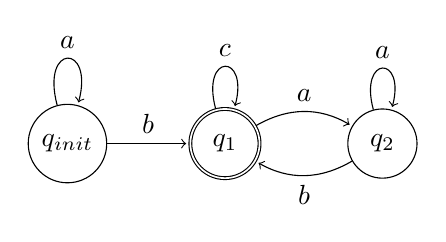
\begin{tikzpicture}[shorten >=1pt, node distance=2cm, on grid, auto]
            % States
            \node[state]   (q0)                {$q_{init}$};
            \node[state, accepting]            (q1) [right=of q0]  {$q_{1}$};
            \node[state] (q2) [right=of q1]  {$q_{2}$};
            
            % Transitions
            \path[->]
                (q0) edge [loop above]   node {$a $}
                (q0)
                     edge []    node {$b $} (q1)
                 (q1) edge [loop above]   node {$c$}
                (q1) edge [bend left]    node {$a$} 
                (q2)
                     
                (q2) edge [loop above]   node {$a $} (q2)
                     edge [bend left]    node {$b$} (q1);
        \end{tikzpicture} \\
        \textbf{(a) A 1-Alphabet DFA: $\Sigma_{1} = \{a,b,c\}$}
    \end{minipage}%
    \hfill
    \begin{minipage}[t]{0.3\linewidth}
        \centering 
        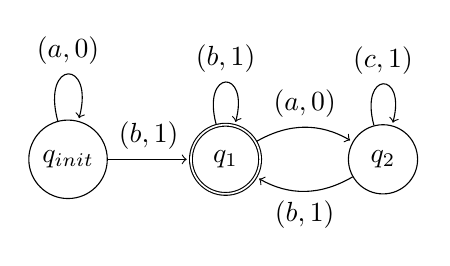
\begin{tikzpicture}[shorten >=1pt, node distance=2cm, on grid, auto]
            % States
            \node[state]   (q0)                {$q_{init}$};
            \node[state,accepting]            (q1) [right=of q0]  {$q_{1}$};
            \node[state] (q2) [right=of q1]  {$q_{2}$};
            
            % Transitions
            \path[->]
                (q0) edge [loop above]   node {$(a,0)$} (q0)
                     edge []    node {$(b,1)$} (q1)
                (q1) edge [bend left]    node {$(a,0)$} (q2)
                     edge [loop above]   node {$(b,1)$} (q1)
                (q2) edge [loop above]   node {$(c,1)$} (q2)
                     edge [bend left]    node {$(b,1)$} (q1);
        \end{tikzpicture} \\
         \textbf{(b) A 2-Alphabet DFA: $\Sigma_{1} = \{a,b,c\},~\Sigma_{2} = \{0,1\}$}
    \end{minipage}
    \hfill
    \begin{minipage}[t]{0.3\linewidth}
        \centering 
        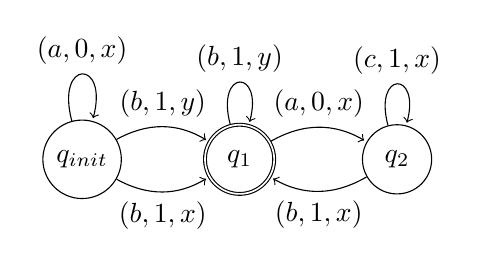
\begin{tikzpicture}[shorten >=1pt, node distance=2cm, on grid, auto]
            % States
            \node[state]   (q0)                {$q_{init}$};
            \node[state, accepting]            (q1) [right=of q0]  {$q_{1}$};
            \node[state] (q2) [right=of q1]  {$q_{2}$};
            
            % Transitions
            \path[->]
                (q0) edge [loop above]   node {$(a,0,x)$} (q0)
                     edge [bend left]    node {$(b,1,y)$} (q1)
                (q0)
                     edge [bend right, below]    node {$(b,1,x)$} (q1)
                (q1) edge [bend left]    node {$(a,0,x) $} (q2)
                     edge [loop above]   node {$(b,1,y)$} (q1)
                (q2) edge [loop above]   node {$(c,1,x)$} (q2)
                     edge [bend left]    node {$(b,1,x) $} (q1);
        \end{tikzpicture} \\
         \textbf{(b) A 3-Alphabet DFA : $\Sigma_{1} = \{a,b,c\},~\Sigma_{2} = \{0,1\},~\Sigma_{2} = \{x,y\}$}
    \end{minipage}
    \caption{A graphical representation of N-Alphabet DFAs. Nodes corresponding to final states are represented by double circles.}
  \label{app:fig:nalphabetdfa}
\end{figure}
 
 \paragraph{Linear Algebra operations over N-Alphabet WAs.} 
 The development of polynomial-time algorithms for computing various SHAP variants for the class of WAs in section \ref{sec:tractable} of the main paper is based on two operations: the projection and the Kronecker product operations. In the following section of the appendix, we will provide a proof of the tractability of their construction.
 
%The construction of a polynomial-time algorithm for computing different SHAP variants for the class of WAs in section \ref{sec:tractable} of the main paper are based on two operations: The projection and the kronecker product operations. In the next section of the appendix, we shall provide a proof of the tractability of their construction.

In addition to these two operators, linear algebra operations over N-Alphabet WAs have also been implicitly utilized in the construction. The closure of 1-Letter WAs under linear algebra operations is a well-established result in the WA literature \citep{droste10}. For completeness, we offer a brief discussion below on how linear algebra operations can be extended to handle multiple alphabets, including their construction and the associated complexity results:

%Besides these two operators, linear algebra operations over N-Alphabet WAs has also been implicitly used in the construction. The closure of 1-Letter WAs under Liner Algebra operations is a classical result in the literature of WAs \citep{droste10}. For the sake of completeness, we provide below a brief discussion on how linear algebra operations over WAs can be generalized to handle multiple alphabets, how they are constructed as well as their associated complexity results:
     \begin{itemize}
         \item \emph{The addition operation:} Given two N-Alpphabet WAs $T = \langle\alpha, \{A_{\sigma_{1},\ldots, \sigma_{N}}\}_{(\sigma_{1}, \ldots, \sigma_{N}) \in \Sigma_{1} \times \ldots \times \Sigma_{N}}, \beta\rangle$ and $T' = \langle\alpha', \{A'_{\sigma_{1},\ldots, \sigma_{N}}\}_{(\sigma_{1}, \ldots, \sigma_{N}) \in \Sigma_{1} \times \ldots \times \Sigma_{N}}, \beta'\rangle$  over $\Sigma_{1} \times \ldots \times \Sigma_{N}$, the N-Alphabet WA, denoted $T + T'$, that computes the function:
         $$f_{T + T'}(w^{(1)}, \ldots, w^{(N)}) = f_{T}(w^{(1)}, \ldots, w^{(N)}) + f_{T'}(w^{(1)}, \ldots, w^{(N)})$$
         is parametrized as follows:
          $$\langle\begin{pmatrix}
              \alpha \\ \alpha'
          \end{pmatrix} , \{\begin{pmatrix}
               A_{\sigma_{1}, \ldots , \sigma_{N}} & \mathbf{O} \\
               \mathbf{O} & A'_{\sigma_{1}, \ldots, \sigma_{N}}
          \end{pmatrix} \}_{(\sigma_{1}, \ldots, \sigma_{N}) \in \Sigma_{1} \times \ldots \times \Sigma_{N}}, \begin{pmatrix}
              \beta \\ \beta' 
          \end{pmatrix} \rangle$$
          The running time of the addition operation is $O(|\Sigma|^{N} \cdot (\texttt{size}(T) + \texttt{size}(T') ))$. The size of the resulting N-Alphabet WA is equal to $O(\texttt{size}(T) + \texttt{size}(T'))$.
          \item \emph{Multiplication by a scalar.} Let $T = \langle\alpha, \{A_{\sigma_{1},\ldots,\sigma_{N}}\}_{(\sigma_{1}, \ldots, \sigma_{N}) \in \Sigma_{1} \times \ldots \times \Sigma_{N}}, \beta\rangle$ be an N-Alphabet WA over $\Sigma_{1} \times \ldots \times \Sigma_{N}$, and a real number $C> 0$, the N-Alphabet WA, denoted $C \cdot T$ that computes the function $f_{C \cdot T}(w^{(1)}, \ldots, w^{(N)}) = C \cdot f_{T}(w^{(1)}, \ldots, w^{(N)})$ is parametrized as: $\langle C \cdot \alpha, \{ A_{\sigma_{1},  \ldots, \sigma_{N}}\}_{(\sigma_{1}, \ldots, \sigma_{N}) \in \Sigma_{1} \times \ldots \times \Sigma_{N}}, \beta \rangle$. It is easy to see that the construction of the N-Alphabet WA $C \cdot T$ runs in $O(1)$ time, and has size equal to the size of $T$. 
     \end{itemize}
  \begin{table}[ht]
  \footnotesize
  	\setlength{\tabcolsep}{0.8em}
    \centering
            \caption{Operations on N-Alphabet WAs, along with their time complexity and output size. The ``In 1'' and ``In 2'' (respectively ``Out'') columns indicate the number of alphabets in the input N-Alphabet WAs for each operation. The ``Time'' column specifies the time complexity of executing the operation, and the ``Output size'' column denotes the size of the resulting N-Alphabet WA after the operation is applied. By convention, a value of $0$ in the ``Output'' and ``Output size'' columns indicates a scalar result.
            %Operations over N-Alphabet WAs, associated with their running time complexity and the size of their outputs. In 1 and In 2 (resp. Out) columns correspond to the number of alphabets of the input N-Alphabet WAs for each operation. The column ``Time'' corresponds to the running time complexity of performing the operation, and the output size refers to the size of the output N-Alphabet WA after applying the operation. By convention, $0$ in the columns 'Output' and ``Output size'' refers to a scalar.
            }
    \begin{tabular}{|c|c|c|c|c|c|}
        \hline
         & \textbf{In 1} & \textbf{In 2} & \textbf{Out} & \textbf{Time} & \textbf{Output size} \\ \hline
        Addition ($+$) & $N$ & $N$ & $N$ & $O(\max\limits_{i \in [N]} |\Sigma_{i}|^{N} \cdot (\texttt{size}(\text{in}_{1}) + \texttt{size}(\text{in}_{2}))$ & $O(\texttt{size}(\text{in}_{1}) + \texttt{size}(\text{in}_{2}))$ \\ \hline
        Scalar Multiplication & $N$ & $0$ & $N$ & $O(1)$ & $O(\texttt{size}(\text{in}_{1})$  \\ \hline
        $\Pi_{0}$ & $1$ & - & $0$ & $O(|\Sigma_{1}| \cdot \texttt{size}(\text{in}_{1})^{2} \cdot n)$ & $0$ \\ \hline
        $\Pi_{1}$ & $1$ & $1$ & $0$ & $O(|\Sigma_{1}| \cdot (| \texttt{size}(\text{in}_{1}) \cdot \texttt{size}(\text{in}_{2}))^{2} \cdot n)$ \footnote{We assume that the operations $\Pi_{0}$ and $\Pi_{1}$ are applied to WAs whose support is equal to $\Sigma^{n}$. This assumption is sufficient for the purpose of our work. In this case, the running time complexity of $\Pi_{0}$ and $\Pi_{1}$ depends on the parameter $n$.} & $0$ \\ \hline
        $\Pi_{i}$ ($i \geq 2$) & $1$ & $N$ & $N-1$ &$O(\max\limits_{i \in [N]} |\Sigma_{i}|^{N} \cdot \texttt{size}(\text{in}_{1}) \cdot \texttt{size}(\text{in}_{2}))$ &  $O(\texttt{size}(\text{in}_{1}) \cdot \texttt{size}(\text{in}_{2}))$ \\ \hline
        $\otimes$ & $N$ & $N$ & $N$ &$O(\max\limits_{i \in [N]} |\Sigma_{i}|^{N} \cdot \texttt{size}(\text{in}_{1}) \cdot \texttt{size}(\text{in}_{2}))$ &  $O(\texttt{size}(\text{in}_{1}) \cdot \texttt{size}(\text{in}_{2}))$ \\ \hline
    \end{tabular}
    \label{app:fig:operationswas}
\end{table}

     A summary of the running time complexity and the size of outputted WAs by all operations over $N$-Alphabet encountered in this work can be found in Table \ref{app:fig:operationswas}. 

\subsection{Proof of proposition \ref{prop:efficentoperations}}
Recall the statement of Proposition \ref{prop:efficentoperations}:

\begin{unumberedproposition}
       Assume that $N = O(1)$. Then, the projection and the Kronecker product operations between $N$-Alphabet WAs can be computed in polynomial time.
\end{unumberedproposition}
 The following result provides an implicit construction of these two operators which implicitly induces the result of Proposition \ref{prop:efficentoperations}: 

\begin{proposition}
Let $N$ be an integer, and $\{\Sigma_{i}\}_{i \in [N]}$, a collection of finite alphabets. We have: 
\begin{enumerate}
 \item The projection operation: Fix an integer $i \in [N]$. Let $A = \langle \alpha, \{A_{\sigma}\}_{\sigma \in \Sigma}, \beta \rangle$ be a WA over $\Sigma_{i}$,  $T = (\alpha', \{A'_{\sigma_{1},\ldots, \sigma_{N}}\}_{(\sigma_{1}, \ldots, \sigma_{N}) \in \Sigma_{1} \times \ldots \times \Sigma_{N}}, \beta')$ be an N-Alphabet WA over $\Sigma_{1} \times \ldots \times \Sigma_{N}$, and $A$ be a WA over $\Sigma_{i}$. The projection of $A$ over $T$ at index $i$, denoted $\Pi_{i}(A,T)$, is parametrized as:
     \begin{align*}
     \Pi_{i}(A,T) :=&  \langle\Sigma_{1} \times \ldots \times \Sigma_{i-1} \times \Sigma_{i} \times \ldots \times \Sigma_{N}, \alpha \otimes \alpha' , \\
     & \{ \sum\limits_{\sigma_{i} \in \Sigma_{i}} A_{\sigma_{i}} \otimes A'_{\sigma_{1}, \ldots, \sigma_{i-1}, \sigma_{i+1}, \ldots, \sigma_{N}} \}_{(\sigma_{1}, \ldots, \sigma_{i-1},\sigma_{i}, \ldots, \sigma_{N}) \in \Sigma_{1} \times \ldots \times \Sigma_{i-1} \times \Sigma_{i+1} \times \ldots \times \Sigma_{N}} ,\beta \otimes \beta'\rangle
     \end{align*}

  \item The Kronecker product operation: Let $T = \langle\alpha, \{A_{\sigma_{1},\ldots, \sigma_{N}}\}_{(\sigma_{1}, \ldots, \sigma_{N}) \in \Sigma_{1} \times \ldots \times \Sigma_{N}}, \beta\rangle$ and $T' = \langle\alpha', \{A'_{\sigma_{1},\ldots, \sigma_{N}}\}_{(\sigma_{1}, \ldots, \sigma_{N}) \in \Sigma_{1} \times \ldots \times \Sigma_{N}}, \beta'\rangle$ be two N-Alphabet WAs over $\Sigma_{1} \times \ldots \times \Sigma_{N}$. The Kronecker product between $T$ and $T'$, $T \otimes T'$, is parametrized as:
  $$T \otimes T' = \langle\alpha \otimes \alpha', \sum\limits_{\sigma \in \Sigma} A_{\sigma_{1}, \ldots, \sigma_{N}} \otimes A'_{\sigma_{1}, \ldots, \sigma_{N}}, \beta \otimes \beta'\rangle$$
\end{enumerate}
\end{proposition}

\begin{proof}
    Let $N$ be an integer, and $\{\Sigma_{i}\}_{i \in [N]}$, a collection of finite alphabets.
    \begin{enumerate}
     \item For the projection operation: Fix $i \in [N]$. Let $T = \langle\alpha', \{A'_{\sigma_{1},\ldots, \sigma_{N}}\}_{(\sigma_{1}, \ldots, \sigma_{N}) \in \Sigma_{1} \times \ldots \times \Sigma_{N}}, \beta'\rangle$ be an N-Alphabet WA over $\Sigma_{1} \times \ldots \times \Sigma_{N}$, and let $A$ be a WA over $\Sigma_{i}$. Let there be some $(w^{(1)}, \ldots, w^{(N)}) \in \Sigma_{1}^{*} \times \ldots \Sigma_{N}^{*}$, such that $|w^{(1)}| = \ldots = |w^{(N)}| = L$. We have:

    \begin{align*}
        f_{\Pi_{i}(A,T)}(w^{(1)}, \ldots, w^{(i-1)}, w^{(i+1)}, w^{(N)}) &= \sum\limits_{w \in \Sigma_{i}^{L}} f_{A}(w) \cdot f_{T}(w^{(1)}, \ldots, w^{(i-1)}, w, w^{(i+1)}, w^{(N)}) \\
        &= \sum\limits_{w \in \Sigma_{i}^{L}} \left( \alpha^{T} \cdot \prod\limits_{j=1}^{L} A_{w_{j}} \cdot \beta \right) \cdot \left( \alpha'^{T} \cdot \prod\limits_{j=1}^{L} A'_{w_{j}^{(1)}, \ldots, w_{j}^{(i)}, \ldots w_{j}^{(N)}} \cdot \beta' \right)  \\
        &= \sum\limits_{w \in \Sigma_{i}^{L}} (\alpha \otimes \alpha')^{T} \cdot \left[ \prod\limits_{j=1}^{L} A_{w_{j}} \otimes A'_{w_{j}^{(1)}, \ldots, w_{j}^{(i)} \ldots w_{j}^{(N)}} \right] \cdot (\beta \otimes \beta') \\
        &= (\alpha \otimes \alpha')^{T} \cdot \prod\limits_{j=1}^{L} \left( \sum\limits_{\sigma \in \Sigma_{i}} A_{\sigma} \otimes A'_{w_{j}^{(1)}, \ldots, \sigma, w_{j}^{(N)}} \right) \cdot (\beta \otimes \beta')
    \end{align*}
    where the third equality is obtained using the mixed-product property of the Kronecker product between matrices.
    \item The Kronecker product operation: Let $T = \langle\alpha, \{A_{\sigma_{1},\ldots, \sigma_{N}}\}_{(\sigma_{1}, \ldots, \sigma_{N}) \in \Sigma_{1} \times \ldots \times \Sigma_{N}}, \beta\rangle$ and $T' = \langle\alpha', \{A'_{\sigma_{1},\ldots, \sigma_{N}}\}_{(\sigma_{1}, \ldots, \sigma_{N}) \in \Sigma_{1} \times \ldots \times \Sigma_{N}}, \beta'\rangle$ be two N-Alphabets WA over $\Sigma_{1} \times \ldots \times \Sigma_{N}$. Let $(w^{(1)}, \ldots, w^{(N)}) \in \Sigma_{1}^{*} \times \ldots \Sigma_{N}^{*}$ such that $|w^{(1)}| = \ldots = |w^{(N)}| = L$. We have:
    \begin{align*}
        f_{T \otimes T'}(w^{(1)}, \ldots, w^{(N)}) &= f_{T}(w^{(1)}, \ldots, w^{(N)}) \cdot f_{T'}(w^{(1)}, \ldots, w^{(N)}) \\
        &= (\alpha^{T} \cdot \prod\limits_{j=1}^{L} A_{w_{j}^{(1)}, \ldots w_{j}^{N}} \cdot \beta) \cdot (\alpha'^{T} \cdot \prod\limits_{j=1}^{L} A'_{w_{j}^{(1)}, \ldots w_{j}^{N}} \cdot \beta') \\
        &=  (\alpha \otimes \alpha')^{T} \cdot \prod\limits_{j=1}^{L} \left( A_{w_{j}^{(1)}, \ldots w_{j}^{N}} \otimes A'_{w_{j}^{(1)}, \ldots w_{j}^{N}} \right) \cdot (\beta \otimes \beta')
    \end{align*}
    where the last equality is obtained using the mixed-product property of the Kronecker product between matrices.
    \end{enumerate}
\end{proof}

\subsection{Proof of Lemma \ref{lemma:shapasoperations}}

In this segment, we provide the proof of the main lemma of section \ref{sec:tractable}:

\begin{unumberedlemma}
Fix a finite alphabet $\Sigma$. Let $f$ be a WA over $\Sigma$, and consider a sequence $(w, w^{\text{reff}}) \in \Sigma^{*} \times \Sigma^{}$ (representing an input and a basline $\x, \x^{\text{reff}} \in \mathcal{X}$) such that $|w| = |w^{\text{reff}}|$. Let $i \in [|w|]$ be an integer, and $\mathcal{D}_P$ be a distribution modeled by an HMM over $\Sigma$. Then:
%Fix a finite alphabet $\Sigma$. Let $f$ be a WA over $\Sigma$, and consider a sequence $(w, w^{\text{reff}}) \in \Sigma^{*} \times \Sigma^{*}$ (representing an input $\x \in \mathcal{X}$ and an auxiliary baseline $\x^{\text{reff}} \in \mathcal{X}$), such that $|w| = |w^{\text{reff}}|$. Additionally, let $i \in [|w|]$ be an integer, and $\mathcal{D}_P$ be a distribution modeled by an HMM over $\Sigma$. We have that:
 %Fix a finite alphabet $\Sigma$. Let $f$ be a WA over $\Sigma$, a sequence $(w,w^{\text{ref}}) \in \Sigma^{*} \times \Sigma^{*}$ (representing an input $\x\in\mathcal{X}$ and an auxialry basline $\x^{\text{ref}}\in\mathcal{X}$) such that $|w| = |w^{\text{ref}}|$, an integer $i \in [|w|]$, and a distribution $\mathcal{D}_P$ modeled by an HMM over $\Sigma$. We have:
         {\small 
            \begin{align*}
         %\emph{\texttt{LOC-I-SHAP}}
         \phi_i
         (f,w,i,\mathcal{D}_P) = \quad\quad\quad\quad\quad\quad\quad\quad\quad\quad\quad\quad\quad\quad\quad\quad \\ \Pi_{1} (A_{w,i}, \Pi_{2}(\mathcal{D}_P, \Pi_{3}(f,T_{w,i}) 
          - \Pi_{3}(f,T_{w}) ) ); \quad\quad \\
            %\end{align*}
            %}
            %{\small 
            %\begin{align*}  
            \Phi_i(f,i,n,\mathcal{D}_P) = \quad\quad\quad\quad\quad\quad\quad\quad\quad\quad\quad\quad\quad\quad\quad\quad \\ 
            \Pi_{0} ( \Pi_{2}(\mathcal{D}_P, A_{i,n} \otimes \Pi_{2}(\mathcal{D}_P, 
             \Pi_{3}(f,T_{i}) - \Pi_{3}(f,T)))); \quad\\
            %\end{align*}
            %}
            %{\small 
            %\begin{align*}
            \phi_b(f,w,i,w^{\text{reff}}) = \quad\quad\quad\quad\quad\quad\quad\quad\quad\quad\quad\quad\quad\quad\quad\quad \\ \Pi_{1} (A_{w,i}, \Pi_{2}(f_{w^{\text{reff}}}, \Pi_{3}(f,T_{w,i}) 
          - \Pi_{3}(f,T_{w})));\quad \\
            %\end{align*}    
            %}
            % {\small 
            %  \begin{align*}
            \Phi_b(f,i,n,w^{\text{reff}},\mathcal{D}_P) = \quad\quad\quad\quad\quad\quad\quad\quad\quad\quad\quad\quad\quad\quad \\ \Pi_{0} ( \Pi_{2}(\mathcal{D}_P, A_{i,n} \otimes \Pi_{2}(f_{w^{\text{reff}}} ,
            \Pi_{3}(f,T_{i}) - \Pi_{3}(f,T)) ))
               \end{align*}
             } where:
    \begin{itemize}
        \item $A_{w,i}$ is a 1-Alphabet WA over $\Sigma_{\#}$ implementing the uniform distribution over coalitions excluding the feature $i$ (i.e., $f_{A_{w,i}} = \mathcal{P}_{i}^{w}$);
        \item $T_{w}$ is a 3-Alphabet \emph{WA} over $\Sigma_{\#} \times \Sigma \times \Sigma$ implementing the function: $ g_{w}(p,w',u) := I(\texttt{do}(p,w',w) = u)$.
        %\begin{equation} \label{eq:Tw}
        %    g_{w}(p,w',u) = I(\texttt{do}(p,w',w) = u)
        %\end{equation}
        \item $T_{w,i}$ is a 3-Alphabet \emph{WA} over $\Sigma_{\#} \times \Sigma \times \Sigma$ implementing the function: $            g_{w,i}(p,w',u) := I(\texttt{do}(\texttt{swap}(p,w_{i},i),w',w) = u)$.
        %\begin{equation} \label{eq:Twi}
        %    g_{w,i}(p,w',u) = I(\texttt{do}(\texttt{swap}(p,w_{i},i),w',w) = u)
        %\end{equation}
        \item $T$ is a 4-Alphabet \emph{WA} over $\Sigma_{\#} \times \Sigma \times \Sigma \times \Sigma$ given as: $g(p,w',u,w) := g_{w}(p,w',u)$.
        %\begin{equation} \label{eq:T}
        %    g(p,w',u,w) = g_{w}(p,w',u)
        %\end{equation}
        \item $T_{i}$ is a 4-Alphabet \emph{WA} over $\Sigma_{\#} \times \Sigma \times \Sigma \times \Sigma$ given as: $ g_{i}(p,w',u,w) := g_{w,i}(p,w',u)$.
        %\begin{equation} \label{eq:Ti}
        %    g_{i}(p,w',u,w) = g_{w,i}(p,w',u)
        %\end{equation}
        \item $A_{i,n}$ is a 2-Alphabet \emph{WA} over $\Sigma_{\#} \times \Sigma$ implementing the function:
         $g_{i,n}(p,w) := I(p \in \mathcal{L}_{i}^{w}) \cdot \mathcal{P}_{i}^{w}(p)$,
         where $|w| = |p| = n$.
       \item $f_{w^{\text{reff}}}$ is an \emph{HMM} such that the probability of generating $w^{\text{reff}}$ as a prefix is equal to $1$.
    \end{itemize}

\end{unumberedlemma}

\begin{proof}

We will prove the complexity results specifically for the cases involving either local or global \emph{Interventional} SHAP. The corresponding proof for local and global Baseline SHAP can be derived by following the same approach as in the interventional case, with the sole modification of replacing $\mathcal{D}_{p}$ with the HMM that models the empirical distribution induced by the reference instance $w^{\text{reff}}$.


%We shall prove the complexity results only for the scenarios considering either local and global \emph{Interventional} SHAP. The same proof for local and global Baseline SHAP can be obtained by mimicking the proof of the interventional case by simply replacing $\mathcal{D}_{p}$ with the HMM modeling the empirical distribution induced by the reference instance $\mathbf{x}^{ref}$.

%Fix a finite alphabet $\Sigma$. Let $M$ be a WA over $\Sigma$, a sequence $w \in \Sigma^{*}$, a integer $i \in [|w|]$, and $P$ a HMM. Let $A_{w,i}$ be a WA and $T_{w},~T_{w,i}$ be two 3-Alphabet WAs as defined in the statement of the lemma. We split the following proof into two segments. The first segment is for the local interventional SHAP version, while the second segment is for the global one.


Fix a finite alphabet $\Sigma$. Let $f$ be a WA over $\Sigma$, $w \in \Sigma^{*}$ a sequence, $i \in [|w|]$ an integer, and $\mathcal{D}_{P}$ an HMM. Define $A_{w,i}$ as a WA and $T_{w},~T_{w,i}$ as two 3-Alphabet WAs as stated in the lemma. We divide the following proof into two parts. The first part addresses the local interventional SHAP version, while the second part covers the global version.







    \begin{enumerate}
        \item For \emph{local Interventional SHAP} we have that:
        \begin{align}
            \phi_i(f,w,i,\mathcal{D}_P) &= \mathbb{E}_{p \sim \mathcal{P}_{i}^{w}} \left[ V_{I}(w,\texttt{swap}(p,w_{i},i), \mathcal{D}_P) - 
 V_{I}(w,p,\mathcal{D}_P) \right] \nonumber \\ 
 &= \sum\limits_{p \in \Sigma_{\#}^{|w|}} f_{A_{w,i}}(p) \left[ \sum\limits_{w' \in \Sigma^{w}} \mathcal{D}_P(w') \cdot \left[ f(\texttt{do}(\texttt{swap}(p,w'_{i},i),w',w)) - f(\texttt{do}(p,w',w)\right] \right] \label{eq:locishap}
        \end{align}
        
 Note that for any $p \in \Sigma_{\#}^{|w|}$ and $(w',u) \in \Sigma^{|w|} \times \Sigma^{|w|}$, we have:
 \begin{equation} \label{eq:obswi}
     f(\texttt{do}(\texttt{swap}(p,w'_{i},i),w',w) = \sum\limits_{u \in \Sigma^{|w|}} f(u) \cdot g_{w,i}(p,w',u) = f_{\Pi_{3}(f,T_{w,i})}(p,w')  
 \end{equation}
 and,
 \begin{equation} \label{eq:obsw}
     f(\texttt{do}(p,w',w)) = \sum\limits_{u \in \Sigma^{|w|}} f(u) \cdot g_{w}(p,w',w) = f_{\Pi_{3}(f,T_{w})}(p,w')
 \end{equation}
 where $g_{w,i}$ and $g_{w}$ are defined implicitly in the body of the lemma statement.

 By plugging equations \eqref{eq:obswi} and \eqref{eq:obsw} in Equation \eqref{eq:locishap}, we obtain:
 \begin{align*}
     \phi_i(f,w,i, \mathcal{D}_P) &=  \sum\limits_{p \in \Sigma_{\#}^{|w|}} f_{A_{w,i}}(p) \left[ \sum\limits_{w' \in \Sigma^{|w|}} \mathcal{D}_P(w') \cdot [ f_{\Pi_{3}(M,T_{w,i})}(p,w') - f_{\Pi_{3}}(M, T_{w}) (p,w') ] \right]
 \end{align*}
 To ease exposition, we employ the symbol $\Tilde{T}$ to refer to the intermediary 2-Alphabet WA over $\Sigma_{\#} \times \Sigma$ defined as:
 $$\Tilde{T} \myeq \Pi_{3}(M,T_{w,i}) - \Pi_{3}(M,T_{w})$$
 Then, we have:
\begin{align*}
    \phi_i(f,w,i, \mathcal{D}_P) &= \sum\limits_{p \in \Sigma_{\#}^{|w|}} f_{A_{w,i}}(p) \left[ \mathcal{D}_P(w') \cdot f_{\Tilde{T}}(p,w') \right] \\
    &= \sum\limits_{p \in \Sigma_{\#}^{|w|}} f_{A_{w,i}}(p) \cdot f_{\Pi_{2}(\mathcal{D}_P,\Tilde{T})}(p) \\
    &= \Pi_{1}(A_{w,i}, \Pi_{2}(\mathcal{D}_P,\Tilde{T}))
\end{align*}
  \item For \emph{Global Interventional SHAP}, the proof follows the same structure as that of the Local version. We hence have that:
 \begin{align}
     \phi_i(f,i,n,P) &= \sum\limits_{w \in \Sigma^{n}} \mathcal{D}_P(w) \cdot \phi_i(f,w,i, \mathcal{D}_P) \nonumber \\
     &= \sum\limits_{w \in \Sigma^{n}}  \mathcal{D}_P(w) \sum\limits_{p \in \Sigma_{\#}}^{|w|} f_{A_{w,i}}(p) \left[ \sum\limits_{w' \in \Sigma^{w}} \mathcal{D}_P(w') \cdot \left[ f(\texttt{do}(\texttt{swap}(p,w'_{i},i),w',w)) - f(\texttt{do}(p,w',w)\right] \right] \label{eq:gloishapwa}
 \end{align}

   Note that for any $p \in \Sigma_{\#}^{n}$ and $(w',u,w) \in \Sigma^{n} \times \Sigma^{n} \times \Sigma^{n}$, we have:
 \begin{equation} \label{eq:obsi}
     f(\texttt{do}(\texttt{swap}(p,w'_{i},i),w',w) = \sum\limits_{u \in \Sigma^{n}} f(u) \cdot g_{i}(p,w',u,w) = f_{\Pi_{3}(M,T_{i})}(p,w',w)  
 \end{equation}
 and,
 \begin{equation} \label{eq:obs}
     f(\texttt{do}(p,w',w)) = \sum\limits_{u \in \Sigma^{|w|}} f(u) \cdot g(p,w',u,w) = f_{\Pi_{3}(M,T)}(p,w',w)
 \end{equation}
 where $g_{i}$ and $g$ are functions defined implicitly in the lemma statement.

 By, again, plugging equations \eqref{eq:obsi} and \eqref{eq:obs} into the equation \ref{eq:gloishapwa}, we obtain:
 \begin{align*}
     \phi_i(f,i,n,P) &= \sum\limits_{w \in \Sigma^{n}} \mathcal{D}_P(w) \cdot \sum\limits_{p \in \Sigma_{\#}^{n}}  f_{A_{i,n}}(p,w) \left[ \sum\limits_{w' \in \Sigma^{n}} \mathcal{D}_P(w') \cdot f_{\Tilde{T}}(p,w',w) \right] \\
     &= \sum\limits_{w \in \Sigma^{n}}  \mathcal{D}_P(w) \cdot \sum\limits_{p \in \Sigma_{\#}^{n}} f_{A_{i,n}}(p,w) \cdot f_{\Pi_{2}(\mathcal{D}_P,\Tilde{T})}(p,w) \\
     &= \sum\limits_{w \in \Sigma^{n}}  \mathcal{D}_P(w) \sum\limits_{p \in \Sigma_{\#}^{n}} f_{A_{i,n} \otimes \Pi_{2}(\mathcal{D}_P,\Tilde{T})}
     (p,w) \\
     &= \sum\limits_{p \in \Sigma_{\#}^{n}} f_{\Pi_{2}(\mathcal{D}_P, A_{i,n} \otimes \Pi_{2}(\mathcal{D}_P,\Tilde{T}))}(p) \\
     &= \Pi_{0} \left( \Pi_{2}(\mathcal{D}_P, A_{i,n} \otimes \Pi_{2}(\mathcal{D}_P,\Tilde{T}))\right)     
  \end{align*} 
    \end{enumerate}
\end{proof}

\subsection{Proof of proposition \ref{prop:nletterwaconstruction}}
In this segment, we shall provide a constructive proof of all machines defined implicitly in Lemma \ref{lemma:shapasoperations}. Formally, we shall prove the following:

\begin{unumberedproposition}
 The N-Alphabet WAs $A_{w,i}$, $T_{w}$, $T_{w,i}$, $T$, $T_{i}$, $A_{i,n}$ and the HMM $f_{w^{\text{reff}}}$ can be constructed in polynomial time with respect to $|w|$ and $|\Sigma|$.
\end{unumberedproposition}
\begin{table}[ht]
    \centering
        \caption{The summary of complexity results (in terms of the length of the sequence to explain $w$ and the size of the alphabet $|\Sigma|$) for the construction of models in proposition \ref{prop:nletterwaconstruction}}
    \begin{tabular}{|c|c|c|c|}
        \hline
         & \textbf{Running Time complexity} & \textbf{Output Size} & \textbf{Output's Alphabet size ($N$)}  \\ \hline
        $A_{w,i}$ & $O(|w|^{3})$ & $O(|w|^{3})$ & $1$  \\ \hline
        $T_{w,i}$ &  $O(|\Sigma|^{3} \cdot |w|)$ & $|w|$ & $3$  \\ \hline
        $T_{w}$ &$O(|\Sigma|^{3} \cdot |w|)$ & $|w|$ & $3$  \\ \hline
        $T_{i}$ & $O(|w|)$ & $O(|w|)$ & $4$  \\ \hline
        $T$ & $O(1)$ & $O(1)$ & $4$ \\ \hline
        $A_{i,n}$ &  $O(|\Sigma|^{2} \cdot |w|^{4})$ & $O(|w|^{4})$ & $2$  \\ \hline
        $f_{w^{reff}}$ & $O(|w|)$ & $O(|w|)$ & $1$  \\ \hline
    \end{tabular}
    \label{app:fig:prop6}
\end{table}
We split the proof of this proposition into four sub-sections. The first sub-section is dedicated to the construction of $A_{w,i}$ and $A_{i,n}$. The second sub-section is dedicated to the construction of $T_{w,i}$ and $T_{i}$. The third sub-section is dedicated to the construction of $T_{i}$ and $T$. The final subsection treats the construction of $f_{w^{reff}}$. The running time of all these constructions as well as the size of their respective outputs are summarized in Table \ref{app:fig:prop6}.  

\subsubsection{The construction of $A_{w,i}$ and $A_{i,n}$} 
Recall $A_{w,i}$ is a WA over $\Sigma_{\#}$ that implements the probability distribution: 
\begin{equation} \label{app:eq:piw}
\mathcal{P}_{i}^{(w)}(p) \myeq \frac{1}{|w|} \sum\limits_{k=1}^{|w|} \mathcal{P}_{i,k}^{(w)}(p)
\end{equation}
where $\mathcal{P}_{i,k}^{(w)}$ is the uniform distribution over patterns belonging to the following set:
$$\mathcal{L}_{i,k}^{(w)} \myeq \{ p \in \Sigma_{\#}^{|w|}: ~ w \in L_{p} \land |p|_{\#} = k \land p_{i} = \# \}$$
The 2-Alphabet WA $A_{i,n}$ can be seen as a global version of $A_{w,i}$ where the sequence $w$ becomes a part of the input of the automaton. Next, we shall provide the construction for $A_{w,i}$. The construction of $A_{i,n}$ is somewhat similar to that of $A_{w,i}$ and will be discussed later on in this section.

\paragraph{The construction of $A_{w,i}$.} Algorithm \ref{app:alg:Awi} provides the pseudo-code for constructing $A_{w,i}$. By noting that the target probability distribution $\mathcal{P}_{i}^{(w)}$ is a linear combination of the set of functions $ \mathcal{F} = \{\mathcal{P}_{i,k}^{(w)}\}$ (Equation \ref{app:eq:piw}), the strategy of our construction  consists at iteratively constructing a sequence of WAs $\{A_{i,k}^{(w)}\}_{k \in [|w|]}$, each of which implements a function $F \in \mathcal{F}$. Thanks to the closure of WAs under linear algebra operations (addition, and multplication with a scalar) and the tractability of implementing them, one can recover the target WA $A_{w,i}$ using linear combinations of the collection of WAs $ \mathcal{A} = \{A_{i,k}^{(w)}\}_{k \in [|w|]}$. 

\begin{algorithm}
\caption{Construction of $A_{w,i}$}
\label{app:alg:Awi}
\begin{algorithmic}[1]
\REQUIRE A sequence $w \in \Sigma^{*}$, An integer $i \in [|w|]$
\ENSURE A WA $A_{w,i}$  
\STATE Initialize $A_{w,i}$ as the empty WA
\FOR{$k = 1 \ldots |w|$}{
  \STATE Construct a DFA $\bar{A}_{i,k}^{|w|}$ that accepts the language $\mathcal{L}_{i,k}^{(w)}$
   \STATE $A_{w,i} \leftarrow A_{w,i} + \frac{1}{|w| \cdot |\mathcal{L}_{i,k}^{|w|}} \cdot \bar{A}_{i,k}^{|w|}$
}
\ENDFOR
\RETURN $A_{w,i}$
\end{algorithmic}
\end{algorithm}


The missing link to complete the construction is to show how each element in the set $\mathcal{A}$ is constructed. For a given $(i,k) \in [|w|]^{2}$, the strategy consists at constructing a DFA that accepts the language $\mathcal{L}_{i,k}^{(w)}$ (denoted $\bar{A}_{i,k}^{|w|}$ in Line 3 of Algorithm~\ref{app:alg:Awi})). Since the function implemented by $A_{i,k}^{(w)}$ represents the uniform probability distribution over patterns in $\mathcal{L}_{i,k}^{(w)}$, then $A_{i,k}^{(w)}$ can be recovered by simply normalizing the DFA $\bar{A}_{i,k}^{(w)}$ by the quantity $\frac{1}{|\mathcal{L}_{i,k}^{(w)}|}$.  

Given a sequence $w \in \Sigma^{*}$ and $(i,k) \in [|w|]^{2}$, the construction of the DFA, $\bar{A}_{i,k}^{(w)}$, is given as follows:
\begin{itemize}
    \item \textbf{The state space:} $Q = [|w|+1] \times \{0, \ldots, |w|\}$ (For a given state $(l,e) \in [|w|] \times [|w|]$, the element $l$ tracks the position of the running pattern, and $e$ computes the number of $\{\#\}$ symbols of the running pattern.
    \item \textbf{Initial State:} $(1,0)$
    \item \textbf{The transition function:} For a given state $(l,e) \in [|w|] \times \{0, \ldots, |w|\}$ and a symbol $\sigma \in \Sigma_{\#}$, we have:
    $$\delta((l,e),\sigma) = \begin{cases}
     (l+1, e+1) & \text{if} ~~\sigma = \# \\
     (l+1,e) & \text{if} ~~\sigma \in \Sigma \land w_{l} = \sigma \land l \neq i
    \end{cases}
    $$
    \item \textbf{The final state:} $F = (|w|+1 , k)$
\end{itemize}

\paragraph{Complexity.} The complexity of constructing $\bar{A}_{i,k}^{(w)}$ for a given $k \in [|w|]$ is equal to $O(|w|^{2})$. Consequently, taking into account the iterative procedure in Algorithm \ref{app:alg:Awi}, this latter algorithm runs in $O(|w|^{3})$. In addition, the size of the resulting $A_{w,i}$ is also $O(|w|^{3})$. 

\paragraph{The construction of $A_{i,n}$.} As previously noted, the 2-Alphabet WA can be interpreted as the global equivalent of $A_{w,i}$. Formally, for an integer $n > 0$ and $i \in [n]$, the 2-Alphabet WA $A_{i,n}$ realizes the function $g_{i,n}$ over $\Sigma_{\#} \times \Sigma$ as defined below:
%As mentioned earlier, the 2-Alphabet WA can be construed as the global counterpart of $A_{w,i}$. Formally, given an integer $n > 0$, and $i \in [n]$, the 2-Alphabet WA $A_{i,n}$ implements the function $g_{i,n}$ over $\Sigma_{\#} \times \Sigma$ given as follows:
\begin{equation} \label{app:eq:gin}
g_{i,n}(p,w) = I(p \in \mathcal{L}_{i}^{w}) \cdot \mathcal{P}_{i}^{w}(p)
\end{equation}

In light of Equation \eqref{app:eq:gin}, the construction of $A_{i,n}$ aligns to the following three step procedure:
\begin{enumerate}
    \item Construct a 2-Alphabet DFA $A'_{w,i}$ over $\Sigma_{\#} \times \Sigma$ that accepts the language $I(p \in \mathcal{L}_{i}^{w})$
    \item Construct a 2-Alphabet WA $\Tilde{A}_{w,i}$ over $\Sigma_{\#} \times \Sigma$ such that: $f_{\Tilde{A}_{w,i}}(p,w) = f_{A_{w,i}}(p)$ (Note that $f_{\Tilde{A}_{w,i}}$ is independent of its second argument)
    \item Return $A'_{w,i} \otimes A_{w,i}$ 
\end{enumerate}

The derivation of the 2-Alphabet WA $\Tilde{A}_{w,i}$ from $A_{w,i}$, whose construction is detailed in Algorithm \ref{app:alg:Awi}, is straightforward. It remains to demonstrate how to construct the 2-Alphabet DFA $A'_{w,i}$ (Step 1).

\paragraph{The construction of $A'_{w,i}$.} Recall that $\mathcal{L}_{i}^{(w)} \myeq \bigcup\limits_{k=1}^{|w|} \mathcal{L}_{i,k}^{(w)}$. Constructing a 2-Alphabet DFA that accepts the language $I(p \in \mathcal{L}_{i}^{w})$ is relatively simple: It involves verifying the conditions $w \in L_{p}$ and $p_{i} = \#$ for the running sequence $(p,w) \in \Sigma_{\#}^{*} \times \Sigma^{*}$. The construction is provided as follows:

%Recall that $\mathcal{L}_{i}^{(w)} \myeq \bigcup\limits_{k=1}^{|w|} \mathcal{L}_{i,k}^{(w)}$. The construction of a 2-Alphabet DFA that accepts the language $I(p \in \mathcal{L}_{i}^{w})$ is relatively straightforward: The conditions $w \in L_{p}$ and $p_{i} = \#$ need to be checked for the running sequence $(p,w) \in \Sigma_{\#}^{*} \times \Sigma^{*}$. It is given as follows:
\begin{itemize}
    \item \textbf{The state space:} $Q = [|w|]$
    \item \textbf{The initial state:} The state $1$
    \item \textbf{The transition function:} For a state $q \in Q$ and $(\sigma,\sigma') \in \Sigma_{\#} \times \Sigma$, then we have that $\delta(q, (\sigma, \sigma')) = q+1$ holds if and only if the predicate: 
     \begin{equation} \label{app:eq:predicate}
      \left(q \neq i \land (\sigma = \#) \lor (\sigma = \sigma') \right) \lor (q = i \land \sigma = \# )
     \end{equation}
     is true.


     
In essence, the predicate defined in Equation~\eqref{app:eq:predicate} captures the idea that, for a given position $q$ in the current pair of sequences $(p,w) \in \Sigma_{\#}^{*} \times \Sigma^{*}$, either $w_{q} \in L_{p_{q}}$ when $q \neq i$ (ensuring the condition $w \in L_p$), or $p_q = \#$ when $q = i$ (ensuring the condition $p_i = \#$).
     
     %Basically, the predicate \eqref{app:eq:predicate} formalizes the fact that for a given position $q$ in the running pair of sequences $(p,w) \in \Sigma_{\#}^{*} \times \Sigma^{*}$, we have that either $w_{q} \in L_{p_{q}}$ if $q \neq i$ (Ensuring the condition $w \in L_{p}$), or $p_{q} = \#$ if $q = 1$ (ensuring the condition $p_{i} = \#$).
    \item \textbf{The final state:} The state $|w|$
\end{itemize}

\paragraph{Complexity.} The construction of $A'_{w,i}$ requires $O(|w|)$ running time, and its size is equal to $O(|w|)$. The running time complexity for the construction of $A_{i,n}$ is dictated by the application of the Kronecker product between the 2-Alphabet WAs $A'_{w,i} \otimes A_{w,i}$ (Step 3 of the procedure outlined above). Given the complexity of computing the Kronecker product between N-Alphabet WAs (see Table \ref{app:fig:operationswas}) and the sizes of $A'_{w,i}$ and $A_{w,i}$, the overall time complexity is equal to $O(|\Sigma|^{2} \cdot |w|^{4})$. The size of $A_{i,n}$ is equal to $O(|w|^{4})$.  

\subsubsection{The construction of $T_{w,i}$ and $T_{w}$} 

The constructions of $T_{w,i}$ and $T_{w}$ are highly similar. Consequently, this section will mainly concentrate on the complete construction of $T_{w,i}$, as it introduces an additional challenge with the inclusion of the \texttt{swap} operation in the function implemented by this 3-Alphabet WA. A brief discussion on the construction of $T_{i}$ will follow at the end of this section, based on the approach used for $T_{w,i}$.

%The construction of $T_{w,i}$ and $T_{w}$ are closely similar. Therefore, this section will primarily focus on the full construction of $T_{w,i}$ as it presents an additional challenge due to the inclusion of the \texttt{swap} operation in the function implemented by this 3-Alphabet WA. A brief note on the construction of $T_{i}$ will be provided at the end of this segment in light of the approach used for $T_{w,i}$.

Recall that $T_{w,i}$ is a 3-Alphabet DFA over $\Sigma_{\#} \times \Sigma \times \Sigma$ that implements the function: 

$$g_{w,i}(p,w',u) = I(\texttt{do}(\texttt{swap}(p,w_{i},i),w',w)= u)$$
for a triplet $(p,w',u) \in \Sigma_{\#}^{*} \times \Sigma^{*} \times \Sigma^{*}$, for which $|p| = |w'| = |u|$.

To ease exposition, we introduce the following predicate:

\begin{equation} \label{app:eq:predicateTwi}
 \Phi(\sigma_{1}, \sigma_{2}, \sigma_{3}, \sigma_{4}) \myeq  \left( \sigma_{1} = \# \land \sigma_{3} = \sigma_{2} \right) \lor \left(\sigma_{1} \neq \# \land \sigma_{3} = \sigma_{4} \right) 
\end{equation}

where $(\sigma_{1}, \sigma_{2}, \sigma_{3}, \sigma_{4}) \in \Sigma_{\#} \times \Sigma \times \Sigma \times \Sigma$. 

The construction of $T_{w,i}$ is given as follows:
\begin{itemize}
    \item \textbf{The state space:} $Q = [|w| + 1]$
    \item \textbf{The initial state:} $q_{init} = 1$
    \item \textbf{The transition function:} For a state $q \in Q$, and a tuple of symbols $(\sigma_{1}, \sigma_{2}, \sigma_{3}) \in \Sigma_{\#} \times \Sigma \times \Sigma$, we have $\delta(q, (\sigma_{1}, \sigma_{2}, \sigma_{3})) = q+1$ if and only if the predicate:
    \begin{equation} \label{app:eq:Twi}
    \left[q \neq i \land \Phi(\sigma_{1},\sigma_{2}, \sigma_{3}, w_{q}) \right] \lor \left[q = i \land \sigma_{3} = w_{q} \right]
    \end{equation}
    is true.
    \item \textbf{The final state:} $|w| + 1$.
\end{itemize}

\textbf{Note.} As previously mentioned, the construction of the 3-Alphabet WA, $T_{w}$, is quite similar to that of $T_{w,i}$. To obtain a comparable construction of $T_{w}$, one can easily adjust the predicate defined in equation~\ref{app:eq:Twi} to $\Phi(\sigma, w_{q}, \sigma_{3}, \sigma_{4})$.
%As mentioned earlier, the construction of the 3-Alphabet WA, $T_{w}$, is closely similar to that $T_{w,i}$. To derive an analogous construction of $T_{w}$, one can simply modify the predicate \ref{app:eq:Twi} to $\Phi(\sigma, w_{q}, \sigma_{3}, \sigma_{4})$.

\subsubsection{The construction of $T_{i}$ and $T$.} 
The 4-Alphabet WAs $T_{i}$ and $T$ can be seen as the global counterparts of $T_{w,i}$ and $T_{w}$, respectively. In addition, their constructions are somewhat simpler than the latter.

\paragraph{The construction of $T_{i}$.} For a given $i \in \mathbb{N}$, the 4-Alphabet WA $T_{i}$ is of size $i$, and constructed as follows: 
\begin{itemize}
     \item \textbf{The state space:} $Q = [i+1]$
    \item \textbf{The initial state:} $q_{init} = 1$
    \item \textbf{The transition function:} For a state $q \in Q$, and $(\sigma_{1}, \sigma_{2}, \sigma_{3}, \sigma_{4}) \in \Sigma_{\#} \times \Sigma \times \Sigma \times \Sigma$, we have:
   $$\delta(q, (\sigma_{1}, \sigma_{2}, \sigma_{3}, \sigma_{4})) = 
   \begin{cases}
       q+1 & \text{if} ~~ [q < i \land \Phi(\sigma_{1}, \sigma_{2}, \sigma_{3}, \sigma_{4})] \lor [q=i \land \sigma_{3} = \sigma_{4}] \\
        i+1 &  \text{if} ~~ q = i+1 \land \Phi(\sigma_{1}, \sigma_{2}, \sigma_{3}, \sigma_{4})
   \end{cases}
   $$
   \item \textbf{The final state:} $i+1$
\end{itemize}


\paragraph{The construction of $T$.} The 4-Alphabet WA $T$ is an automaton with a single state, formally defined as follows:
\begin{itemize}
    \item \textbf{The state space:} $Q = \{1\}$,
    \item \textbf{The initial state:} $q_{init} = 1$.
    \item \textbf{The transition function:} For $(\sigma_{1}, \sigma_{2}, \sigma_{3}, \sigma_{4}) \in \Sigma_{\#} \times \Sigma \times \Sigma \times \Sigma$, we have that:
    $\delta(1, (\sigma_{1}, \sigma_{2}, \sigma_{3}, \sigma_{4})) = 1$ holds, if and only if the predicate $\Phi(\sigma_{1}, \sigma_{2}, \sigma_{3}, \sigma_{4})$ is true. 
\end{itemize}

\subsubsection{The construction of $f_{w^{reff}}$}
Given a sequence $w^{ref} \in \Sigma^{*}$, the machine $f_{w^{reff}}$ is defined as an HMM such that the probability of generating the sequence $w^{ref}$ as a prefix is equal to 1. The set of HMMs that meet this condition is infinite. In our case, we opt for an easy construction of an HMM, denoted $f_{w^{reff}}$, belonging to this set.

The state space of $f_{w^{reff}}$ is given as $Q = [|w_{ref}| + 1]$ states. Similarly to the constructions above, each state is associated with a position within the emitted sequence of the HMM. Its functioning mechanism can be described using the following recursive procedure: 
\begin{itemize}
    \item The HMM starts from the state $q = 1$ with probability $1$. The probability of emitting the symbol $w^{ref}_{1}$ and transitioning to the state $q= 2$ is equal to $1$.
    \item For $q \in [|w^{ref}|]$, the probability of generating the symbol $w^{ref}_{q}$ and transitioning to the state $q+1$ is equal to $1$.
\end{itemize}
When the HMM reaches the state $|w^{ref}| + 1$, it generates a random symbol in $\Sigma$ and remains at state $|w^{ref}| + 1$ with probability 1. One can readily verify (by a straightforward induction argument) that this HMM generates infinite sequences prefixed by the sequence $w^{ref}$ with probability 1. 

\paragraph{Complexity.} The running time of this construction is equal to $O(|w^{ref}|)$, and the size of the obtained HMM $f_{w^{reff}}$ is equal to $O(|w^{ref}|)$.
 \section{From Sequential Models to Non-Sequential Models: Reductions and Inter-inclusions} \label{app:reductiontree}
%\textcolor{red}{This section requires some text editing, notation harmonisation etc. 
%I believe it's well-structured and the technical stuff is fairly correct but it requires some editing refinements, clarifications etc.
%Note that this section relies heavily on background of section \ref{app:sec:terminology}(Models and Distributions).
%}


In Section~\ref{subsec:tree2WA} of the main paper, we demonstrated how the tractability result for computing various SHAP variants for WAs extends to several non-sequential models, including Ensemble Trees for Regression and Linear Regression Models (Theorem~\ref{cor:reductions}). In this section, we will present a complete and rigorous proof of this connection, along with additional theoretical insights into the relationships between these models and distributions. Specifically:



%In section \ref{subsec:tree2WA} of the main article, we showed how the tractability result of computing different SHAP variants for WAs is projected on several non-sequential models such as Ensemble Trees for Regression and Linear Regression Models (Theorem \ref{cor:reductions}). This section is dedicated to provide theoretical insights into this connection: 

\begin{enumerate}
\item 
In the first subsection, we establish the proof of Theorem~\ref{cor:reductions}. This proof is based on several reductions, including those from linear regression models and ensemble trees to weighted automata, as well as from empirical distributions to the family $\overrightarrow{\texttt{HMM}}$.


%In the first subsection, we prove the result of Theorem \ref{cor:reductions}. This result will rely on several reductions from Linear regression models and ensemble trees to Weighted Automata and from empirical distributions to the family $\overrightarrow{\texttt{\text{HMM}}}$. 
\item In the second subsection, we present additional reductions that, while not explicitly used to prove the complexity results stated in the article, showcase the expressive power of the HMM class in modeling various families of distributions relevant to SHAP computations. These include distributions represented by Naive Bayes models and Markovian distributions. Moreover, we will highlight certain complexity results, listed in Table~\ref{fig:summaryresults}, that were not directly mentioned in the main text but are illuminated by these reduction findings.

%In the second subsection, we prove other reductions which weren't used explicitly to prove complexity results stated in the article, but highlights the expressiveness power of the class of HMMs to model various family of distributions encountered in works related to SHAP computations, including distributions modeled by Naive Bayes Models and Markovian Distributions. Additionally, we will highlight some complexity results presented in Table \ref{fig:summaryresults} but weren't explicitly mentionned in the main article in light of these reduction results.  

\end{enumerate} 

\subsection{Proof of Theorem \ref{cor:reductions}}

Recall the statement of Theorem \ref{cor:reductions}:

\begin{unumberedtheorem}
        Let $\mathbb{S}:= \{ \emph{\texttt{LOC}}, \emph{\texttt{GLO}} \}$, $\mathbb{V} := \{\texttt{\emph{B}}, \texttt{\emph{I}}\}$, $\mathbb{P}:= \{ \texttt{\emph{EMP}}, \overrightarrow{\emph{\texttt{HMM}}} \} $, and $\mathbb{F}:= \{\emph{\texttt{DT}}, \emph{\texttt{ENS-DT}}_{\emph{\texttt{R}}}, \emph{\texttt{Lin}}_{\emph{\texttt{R}}}\}$. Then, for any \emph{\texttt{S}} $\in \mathbb{S}$, $\texttt{\emph{V}} \in \mathbb{V}$, $\texttt{\emph{P}} \in \mathbb{P}$, and $\emph{\texttt{F}}\in \mathbb{F}$ the problem  $\emph{\texttt{S-V-SHAP}}(\emph{\texttt{F}}, \texttt{\emph{P}})$ can be solved in polynomial time.
\end{unumberedtheorem}

The proof of this theorem will rely on four inter-model polynomial reductions:

\begin{unumberedclaim}
The following statements hold true:
\begin{enumerate}
    \item $\overrightarrow{\texttt{\emph{HMM}}} \preceq_{\emph{P}} 
\texttt{\emph{HMM}}$
   \item $\texttt{\emph{EMP}} \preceq_{\emph{P}} \overrightarrow{\texttt{\emph{HMM}}}$ 
   \item $\texttt{\emph{ENS-DT}}_{\texttt{\emph{R}}}\preceq_{\emph{P}} \texttt{\emph{WA}}$
   \item $\texttt{\emph{LIN}}_{\texttt{\emph{R}}} \preceq_{\emph{P}} \texttt{\emph{WA}}$
\end{enumerate}
\end{unumberedclaim}

Theorem \ref{cor:reductions} is a direct consequence of the following four claims. This section is structured into four parts, each dedicated to proving one of these claims. Without loss of generality and to simplify the notation, we will assume throughout that all models operate on binary inputs. However, it is important to note that all of our results can be extended to the setting where each input is defined over $k$ discrete values.

%follows directly from these four claims. The rest of this section is divided into four parts, with each part proving one of these claims. Without a loss of generality, we assume in the sequel that all models operate on binary inputs. 

\subsubsection{Claim 1: $\overrightarrow{\texttt{\text{HMM}}}$ is polynomially reducible to $\texttt{\text{HMM}}$}

Consider a model $\ar{\tt{\text{M}}} = \langle \pi, \alpha, \{T_{i}\}_{i \in [n]}, \{O_{i}\}_{i \in [n]}\rangle$, where the size of $\ar{\text{M}}$ is denoted as $m$. This model $\ar{\text{M}}$ encodes a probability distribution over the hypercube $\{0,1\}^{n}$. The goal is to prove that a model $M \in \ttt{\text{HMM}}$, which satisfies the following condition:

\begin{equation} \label{app:eq
} P_{\ar{\text{M}}}(x_{1}, \ldots, x_{n}) = P_{\text{M}}^{(n)}(x_{1}, \ldots, x_{n}), \end{equation}

can be constructed in polynomial time with respect to the size of $\ar{\text{M}}$. Intuitively, this condition asserts that the probability of generating a sequence $x = x_{1}, \ldots, x_{n}$ of length $n$ using $M$ is the same as the probability of generating $(x_{1}, \ldots, x_{n})$ using $\ar{\text{M}}$.



%Fix a model $\ar{\tt{\text{M}}} = \langle \pi, \alpha, \{T_{i}\}_{i \in [n]}, \{O_{i}\}_{i \in [n]}\rangle$ where $\texttt{size}(\ar{\text{M}}) = m$. The model $\ar{\text{M}}$ that encodes a probability distribution over the hypercube $\{0,1\}^{n}$. The objective is to prove that a model $M \in \ttt{\text{HMM}}$ satisfying the following condition:

%\begin{equation} \label{app:eq:hmm2hmm}
%P_{\ar{\text{M}}}(x_{1}, \ldots, x_{n}) = P_{\text{M}}^{(n)}(x_{1} \ldots x_{n} )
%\end{equation}

%can be constructed in polynomial-time with respect to the size of $\ar{\text{M}}$.


%Intuitively, this condition means that the probability of generating a prefix $x = x_{1} \ldots x_{n}$ of length $n$ by $M$ is equal to the probability of generating $(x_{1}, \ldots, x_{n})$ by $\ar{\text{M}}$.

%\textcolor{blue}{@Shahaf: Basically, this condition means that the probability of generating a prefix $x = x_{1} \ldots x_{n}$ of length $n$ by $M$ is equal to the probability of generating $(x_{1}, \ldots, x_{n})$ by $\ar{\text{M}}$} 

%can be constructed in polynomial-time with respect to the size of $\ar{\text{M}}$.

The construction aims to build an HMM $M$ that simulates $\ar{\text{M}}$ up to position $n$. Afterward, $M$ transitions into a dummy hidden state where it stays stuck permanently, emitting symbols uniformly at random. To simulate $\ar{\text{M}}$ within the support $\{0,1\}^{M}$, $M$ must keep track of both the state reached by $\ar{\text{M}}$ after emitting a prefix $x_{\pi{1}}, \ldots x_{\pi{j}}$ for a given $j \in [n]$, and the position reached in the sequence. Once the $n$-th symbol has been emitted, the HMM $\text{M}$ transitions into a dummy state, which emits symbols uniformly at random and remains in that state indefinitely. The detailed construction is provided as follows:


%The idea of the construction is to create an HMM $M$ that simulates $\ar{\text{M}}$ up to the position $n$. Afterwards, $M$ transitions to a dummy hidden state where it remains stuck forever, emitting symbols uniformly at random. To simulate $\ar{\text{M}}$ inside the support $\{0,1\}^{M}$, $M$ needs to keeps track of both the state reached by $\ar{\text{M}}$ after emitting a prefix $x_{\pi{1}}, \ldots x_{\pi{j}}$ for a given $j \in [n]$ as well as the reached position in the sequence. After emitting the $n$-th symbol, the HMM $\text{M}$ transitions to a dummy state that emits a symbol uniformly at random and remains stuck in this state forever. The details of the construction are given as follows:

\begin{itemize}
    \item \textbf{The state space:} $Q = [M] \times [n+1]$
    \item \textbf{State initialization:} The HMM $M$ begins generating from the state $(i,1)$ for $i \in [M]$ with a probability of $\alpha(i)$.
    
    %the HMM $M$ starts generating from the state $(i,1)$ for $i \in [M]$ with probability equal to $\alpha(i)$
    \item \textbf{The transition dynamics:} For $(i,k,j) \in [M]^{2} \times [N]$, the HMM $M$ transitions from state $(i,j)$ to state $(k,j+1)$ with a probability of $T_{j}[i,k]$. Additionally, for any $i \in [M]$, we have $T[(i,n+1), (i,n+1)] = 1$ (meaning the HMM remains in the dummy state $n+1$ indefinitely).
    %For $(i,k,j) \in [M]^{2} \times [N]$, the HMM $M$ transitions from the state $(i,j)$ to the state $(k,j+1)$ with probability equal to $T_{j}[i,k]$. On the other hand, for any $i \in [M]$, we have $T[(i,n+1), (i,n+1)] = 1$ (i.e. the HMM stays in the dummy state $n+1$ forever).
    \item \textbf{Symbol emission:} At a state $(i,j) \in [M] \times [n]$, the probability of emitting the symbol $\sigma$ is equal to $O_{\pi(i)}[i,\sigma]$. On the other, for any state $(i,n+1)$ where $i \in [M]$, the HMM $M$ generates the symbol $\sigma$ uniformly at random. 
\end{itemize}

\subsubsection{Claim 2: \texttt{EMP} is polynomially reducible to $\overrightarrow{\texttt{HMM}}$}
% Introduction of the content of this section

The purpose of this subsection is to demonstrate that the class of Empirical distributions can be polynomially reduced to the \texttt{HMM} family. This claim has been referenced multiple times throughout the main article, where it played a key role in deriving complexity results for computing SHAP variants across various ML models, including decision trees, linear regression models, and tree ensemble regression models. Specifically, it shows that computing these variants under distributions modeled by HMMs is at least as difficult as computing them under empirical distributions. %We begin by revisiting the concept of empirical distributions (in the context of models with boolean input features):

%The goal of this subsection is to show that the class of Empirical distributions is polynomially reducible to the family \texttt{HMM}. This claim has been used in several parts of the main article, where it was useful to deduce compelxity results of computing SHAP variants of different ML models such as decision trees, linear regression models, and tree ensemble regression models, under distributions modeled by HMMs are at least as hard as computing these variants under empirical distributions. We first recall what is meant by empirical distributions (in the context of models with boolean input features): 

% Introduction of the empirical distribution 

% The strategy consists of 2 steps: Shalllow description of these steps 
%The strategy of reducing empirical distributions into distributions modeled by the family $\overrightarrow{\text{HMM}}$ comprises two steps:

The strategy for reducing empirical distributions to those modeled by the $\overrightarrow{\text{HMM}}$ family involves two steps:

\begin{enumerate}
    \item The sequentialization step, which aims to transform the vectors in $\mathcal{D}$ into a dataset of binary sequences, referred to as $\texttt{SEQ}(\mathcal{D})$.
    %The sequentialization step: The objective of this step is to convert vectors in $\mathcal{D}$ into a dataset of binary sequences, denoted $\texttt{SEQ}(\mathcal{D})$.
    \item The construction of a  model in $\overrightarrow{\text{HMM}}$ that encodes the empirical distribution induced by $\texttt{SEQ}(\mathcal{D})$.  
\end{enumerate}

We will now provide a detailed explanation of each step:

% The first step (Sequentialization) is relatively easy .. 
\emph{Step 1 (The sequentialization step):} The sequentialization step is fairly straightforward and has been utilized in \cite{marzouk24a} to transform decision trees into equivalent WAs. The sequentialization operation, denoted as $\texttt{SEQ}(.,.)$, is defined as follows:
%The sequentialization step is relatively easy and has been used in the work of \cite{marzouk24a} to reduce decision trees into equivalent WAs. Define the sequentialization operation $\texttt{SEQ}(.,.)$ as: 
$$\texttt{SEQ}(\overrightarrow{x}, \pi) = x_{\pi(1)} \ldots x_{\pi(N)}$$

where $\pi$ is a permutation. Essentially, the $\texttt{SEQ}(.,.)$ operation transforms a given vector in $\{0,1\}^{N}$ into a binary string, with the order of the feature variables determined by the permutation $\pi$. From here on, without loss of generality, we assume $\pi$ to be the identity permutation.

%where $\pi$ is a permutation. Basically, the $\texttt{SEQ}(.,.)$ operation converts a given vector in $\{0,1\}^{N}$ into a binary string where the ordering of feature variables is dictated by the permutation $\pi$. In the sequel, without a loss of generality, we assume $\pi$ to be the identity permutation. 

% The second step : Description of PTAs, Conversion of EMP to PTAs  
\emph{Step 2 (The construction of the HMM):} 
Applying the sequentialization step to the dataset $\mathcal{D}$ results in a \emph{sequentialized} dataset consisting of $M$ binary strings, denoted as $\texttt{SEQ}(\mathcal{D})$. The goal of the second step in the reduction is to construct a model in $\overrightarrow{HMM}$ that models the empirical distribution induced by $\texttt{SEQ}(\mathcal{D})$. While this construction is well-known in the literature of Grammatical Inference (refer to
La Higuera book on Grammatical Inference), we will provide the details of this construction below. 

%Applying the sequentialization step on the dataset $\mathcal{D}$ yields a \emph{sequentialized} dataset comprised of $M$ binary strings denoted $\texttt{SEQ}(\mathcal{D})$. The objective of the second step of the reduction consists at constructing a PPTA that models the empirical distribution induced by $\texttt{SEQ}(\mathcal{D})$. Although this construction is folklore in the litterature of Grammatical Inference [ref:de La Higuera book Grammatical Inference], we provide next the details of this construction.

For a given sequence $w$, we denote the number of occurences of $w$ as a prefix in the dataset $P(\mathcal{D})$ as:
$$N(w) \myeq \#|\{x \in \texttt{SEQ}(\mathcal{D}): ~ \exists (s) \in \{0,1\}^{*}: x = ws\}|$$

We also define the set of prefixes appearing in $\texttt{SEQ}(\mathcal{D})$ as the set of all sequences $w \in \{0,1\}^{*}$ such that $N(w) \neq 0$. This set shall be denoted as $\text{P}(\mathcal{D})$. Note that the set $\text{P}$ is prefix-closed \footnote{A set of sequences $S$ is prefix-closed if the set of prefixes of any sequence in $S$ is also in $S$}.

A (stationary) model in $\overrightarrow{\text{HMM}}$ that encodes the empirical distribution induced by the dataset $\texttt{SEQ}(\mathcal{D})$ is a probabilistic finite state automaton parametrized as follows: 
\begin{enumerate}
    \item \textbf{The permutation:} The identity permutation.
    \item \textbf{The state space:} $Q = \text{P}(\mathcal{D})$.
    \item \textbf{The initial state vector:} Given $\sigma \in \{0,1\}$, the probability of starting from the state $\sigma \in \text{P}(\mathcal{D})$ is equal to $\frac{N(\sigma)}{|\mathcal{D}|}$.
    \item \textbf{The transition dynamics:} For a state $w \sigma \in Q$, where $w \in Q$ \footnote{Thanks to the prefix-closedness property of the set $\text{P}(\mathcal{D})$, if $w\sigma$ is in $Q$, then $w$ is also in $Q$.} and $\sigma \in \Sigma$,  the probability of transitioning from the state $w$ to the state $w\sigma$ is equal to $\frac{N(w \sigma)}{N(w)}$. 
    \item \textbf{The symbol emission:} For any state $w \sigma \in Q$, where $w \in Q$ and $\sigma \in \{0,1\}$, the probability of generating the symbol $\sigma$ from the state $w\sigma$ is equal to $1$.
 \end{enumerate}

One can readily prove that the resulting model computes the empirical distribution induced by $\text{P}(\mathcal{D})$. Indeed, by construction, the probability of generating a binary sequence $w$ by the model is equal to the probability of generating the sequence of states $w_{1}, w_{1:2}, \ldots, w_{1:n-1} w$. The probability of generating this state sequence is equal to:
$$\frac{N(w_{1})}{|\mathcal{D}|} \prod\limits_{i=1}^{|w|} \frac{N(w_{1:i+1})}{N(w_{1:i})} = \frac{N(w)}{|\mathcal{D}|}$$

\subsubsection{Claim 3: \texttt{DT} and $\texttt{\text{ENS-DT}}_{\texttt{\text{R}}}$ are polynomially reducible to \texttt{WA}}
%\textcolor{blue}{@Shahaf: In my old writing of this section, Tree-based models designate both decision trees and ensemble trees for regression in your new formulation.}

The construction of an equivalent WA for either a decision tree or a tree ensemble used in regression tasks (i.e., a model in \texttt{DT} or a model in $\texttt{\text{ENS-DT}}_{\text{R}}$) is built upon the following result provided in \cite{marzouk24a} for the \texttt{DT} family:

%The construction of an equivalent WA to either a decision tree or a tree ensemble used for regression tasks (i.e. a model in \texttt{DT} or a model in $\texttt{\text{ENS-DT}}_{\text{R}}$) is based on top of the following result provided in \cite{marzouk24a} for the family of \texttt{DT}:

\begin{proposition} \label{app:prop:DT2WA}
    There exists a polynomial-time algorithm that takes as input a decision Tree $T \in \texttt{\emph{DT}}$ over the binary feature set $X = \{X_{1}, \ldots, X_{n} \}$ and outputs a WA $A$ such that:
     $$f_{A}(x_{1}\ldots x_{n}) = f_{T}(x_{1}, \ldots, x_{n} )$$
\end{proposition}


Since an ensemble of decision trees used for regression tasks is a linear combination of decision trees, and the family of WAs is closed under linear combination operations, with these operations being implementable in polynomial time as demonstrated in section~\ref{app:sec:ter}, Proposition~\ref{app:prop:DT2WA} consequently implies the existence of a polynomial-time algorithm that produces a WA equivalent to a given tree ensemble model used for regression.

%Given that an ensemble of deicision trees used for regression taks is a linear combination of a collection of decision trees, and that the family of WAs is closed under linear combination operations and implementing these linear operations can be performed in polynomial time as shown in section \ref{app:sec:ter}, Proposition \ref{app:prop:DT2WA} implies as a corollary the existence of a polynomial-time algorithm that returns a WA equivalent to a given tree ensemble model used for regression.

\paragraph{Complexity.} The algorithm for constructing a WA equivalent to a given DT $T$ runs in $O(|T|)$, where $|T|$ denotes the number of edges in the DT $T$. The size of the resulting WA is $O(|T|)$ (See \cite{marzouk24a} for more details). Consequently, the overall algorithm for constructing an equivalent regression tree ensemble consisting of $m$ DTs $\{T_{i}\}_{i \in [m]}$ operates in $O(m \cdot \max\limits_{i \in [m]} |T_{i}|)$. The size of the ensemble is also $O(m \cdot \max\limits_{i \in [m]} |T_{i}|)$.

%The algorithm for constructing an equivalent WA to a given DT $T$ runs in $O(|T|)$ where $|T|$ refers to the number of edges of the DT $T$. The size of the resulting WA is $O(|T|)$ (See \cite{marzouk24a} for full details). Consequently, the overall algorithm of constructing an equivalent regression tree ensemble comprised of an ensemble of $m$ DTs $\{T_{i}\}_{i \in [m]}$ is given as $O(m \cdot \max\limits_{i \in [m]} |T_{i}|)$. Its size is likewise equal to $O(m \cdot \max\limits_{i \in [m]} |T_{i}|)$. 



\subsubsection{Claim 4: $\texttt{\text{Lin}}_{\texttt{\text{R}}}$ is polynomially reducible to \texttt{WA}.}

Let $M := \langle \{w_{i,d}\}_{i \in [n], d \in \mathbb{D}_{i}}, b\rangle$ be a linear regression model over the finite set $\mathbb{D} = [m_{1}] \times \ldots [m_{n}]$ where $\{m_{i}\}_{i \in [n]}$, computing the function (as defined earlier):

%Let $M := \langle \{w_{i,d}\}_{i \in [n], d \in \mathbb{D}_{i}}, b\rangle$ be linear regression model over the finite set $\mathbb{D} = [m_{1}] \times \ldots [m_{n}]$ where $\{m_{i}\}_{i \in [n]}$ computing the function (as was defined earlier):

$$f(x_{1}, \ldots , x_{n}) = \sum\limits_{i=1}^{n} \sum\limits_{d \in \mathbb{D}_{i}} w_{i,d} \cdot I(x_{i}=d) + b$$


For the purposes of our reduction to WAs, we will assume that: $m_{1} = \ldots = m_{n} = m$.
The conversion of a linear regression model $M$ over the input space $\mathbb{D} = [m_{1}] \times \ldots [m_{n}]$ to an equivalent one over $[m]^{n}$ can be done as follows: We set $m$ to be $\max\limits_{i\in [n]} m_{i}$, and the parameters $\{\tilde{w}_{i,d}\}_{i \in [n], d \in [m]}$ for the new model are set as:

%For the sake of our reduction to WAs, we shall assume that: $m_{1} = \ldots = m_{n} = m$.
%The conversion of a linear regression model $M$ over the input space $\mathbb{D} = [m_{1}] \times \ldots [m_{n}]$ to an equivalent one over $[m]^{n}$ can be performed as follows: We set $m$ as $\max\limits_{i=1}^{n} m_{i}$ and we set the parameters $\{\tilde{w}_{i,d}\}_{i \in [n], d \in [m]}$ for the new model as:   

$$\tilde{w}_{i,d} = \begin{cases}
    w_{i,d} & \text{if} ~~ d \leq m_{i} \\
    0 & \text{otherwise}
\end{cases}$$


Observe that this procedure operates in $O(\max\limits_{i \in [n]} m_{i})$ time.

\paragraph{Reduction strategy.} For a given linear regression model $M := \langle\{w_{i,d}\}_{i \in [n], d \in [m]},b\rangle$ over $[m]^{n}$, we construct a WA over the alphabet $\Sigma = [m]$ with $n+1$ states. The initial state vector has value $1$ for state $1$, and $0$ for all other states. For $i \in [n]$, the transition from state $i$ to state $i+1$ is assigned a weight of $w_{i,\sigma}$ when processing the symbol $\sigma$ from this state. Figure~\ref{app:fig:lin2wa} illustrates an example of the graphical representation of the resulting WA from a given linear regression tree.

%For a given linear regression model $M = \langle\{w_{i,d}\}_{i \in [n], d \in [m]},b\rangle$ over $[m]^{n}$, we construct a WA over the alphabet $\Sigma = [m]$ of $n+1$ states. The initial state vector is equal to $1$ for the state $1$, and $0$ for all the others. For $i \in [n]$, a transitions from the state $i$ to the state $i+1$ is assigned a weight equal to $w_{i,\sigma}$ when processing the symbol $\sigma$ from this state. Figure \ref{app:fig:lin2wa} illustrates an example of the graphical representation of the resulting WA from a given linear regression tree.



The additive intercept parameter $b$ can be incorporated into this constructed model by simply adding the resulting WA from the procedure described above to a trivial single-state WA that outputs the value $b$ for all binary strings (see Section~\ref{app:sec:ter} for more details on the addition operation between two WAs).

%The incorporation of the additive intercept parameter $b$ in this constructed model can be straightforwardly obtained by performing an addition operation over this resulting WA of the procedure outlined above and the trivial single state WA that output the value $b$ to all binary strings (see Section \ref{app:sec:ter} for further details of the addition operation over 2 WAs). 
\begin{figure}[h]
    \centering
    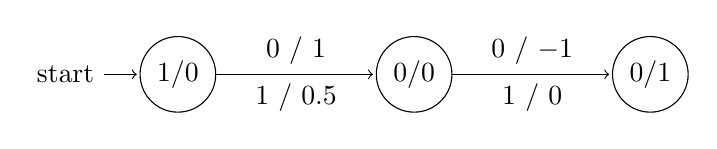
\begin{tikzpicture}[shorten >=1pt, node distance=3cm, on grid, auto]

      % States
      \node[state, initial] (q_1) {$1/0$};
      \node[state] (q_2) [right=of q_1] {$0/0$};
      \node[state] (q_3) [right=of q_2] {$0/1$};

      % Transitions
      \path[->] (q_1) edge node[above] {0 / $1$} 
                         node[below] {1 / $0.5$} (q_2);
      \path[->] (q_2) edge node[above] {0 / $-1$} 
                         node[below] {1 / $0$} (q_3);

    \end{tikzpicture}
    \caption{A construction of a WA equivalent to a linear regression over $2$ binary features with the following weights: $w_{1,0} = 1,~w_{1,1}=0.5,~w_{2,0}=-1,~w_{2,1}=0$. The notation $x/y$ within the state nodes represents the initial weight of the state ($x$) and the final weight of the state ($y$).
    %A construction of a WA equivalent to a linear regression over $2$ binary features with the weights: $w_{1,0} = 1,~w_{1,1}=0.5,~w_{2,0}=-1,~w_{2,1}=0$. The notation $x/y$ inside the state nodes corresponds to the initial weight of the state ($x$) and the final weight of the state ($y$).
    }
    \label{app:fig:lin2wa}
\end{figure}

\subsection{Additional reduction results and implications on SHAP computation}
Some of the complexity results presented in Table~\ref{fig:summaryresults} were not explicitly discussed in the main article. Instead, additional polynomial-time reductions between Hidden Markov Models and other families of distributions are needed to derive them. For completeness, we include in the first part of this subsection proofs of these reduction relationships. Following that, we outline the implications of these relationships on the complexity of certain SHAP configurations shown in Table~\ref{fig:summaryresults}.


%Some complexity results highlighted in Table \ref{fig:summaryresults} weren't explicitly stated in the main article. Instead, additional polynomial-time reductions  between Hidden Markov Models and other families of distributions are required to derive them.  For the sake of completeness, we provide in the first segment of this section proofs of these reduction relationships. Afterwards, we highlight the implications of these relations on the complexity of some SHAP configurations present in Table \ref{fig:summaryresults}. 

\subsubsection{Additional reduction results}

An interesting aspect of Hidden Markov Models is that they provide a unifying probabilistic modeling framework encompassing several families of distributions discussed in the literature on SHAP computation. Specifically, the class \texttt{MARKOV} (and, \textit{de facto}, the family \texttt{IND}, which is trivially a subclass of \texttt{MARKOV}) as well as \texttt{NB} (more formally, $\texttt{NB} \preceq_{P} \ar{\texttt{\text{HMM}}}$) can be polynomially reduced to the class of Hidden Markov Models.

%An interesting feature of Hidden Markov Models  offer a unifying probabilistic modeling framework that covers several families of distributions covered in the literature regarding SHAP computation. In particular, the class \texttt{MARKOV}, (and, \textit{de facto} the family \texttt{IND}, this latter being trivially a sub-class of \texttt{MARKOV}) and \texttt{NB} (more rigorously, $\texttt{NB} \preceq_{P} \ar{\texttt{\text{HMM}}}$) can be polynomially reduced to the class of Hidden Markov Models. 

\paragraph{Claim 1: \texttt{NB} is  polynomially reducible to $\overrightarrow{\texttt{HMM}}$.}

Let $M \in \texttt{NB}$ be a model over $n$ binary features with a hidden variable $Y$ that takes values from the discrete set $[m]$. The goal is to construct, in polynomial time, a model $M' \in \ar{\texttt{\text{HMM}}}$ that is equivalent to $M$, i.e.:

%Let there be some $M \in \texttt{NB}$ over $n$ binary features with a hidden variable $Y$ taking values from the discrete set $[m]$. The objective is to construct in polynomial time a  model $M' \in \ar{\texttt{\text{HMM}}}$ equivalent to $M'$, i.e.:

$$\forall (x_{1}, \ldots, x_{n}) \in \{0,1\}^{n}:~~P_{M}(x_{1}, \ldots, x_{n}) = P_{M'}(x_{1}, \ldots , x_{n})$$

A key observation underlying the reduction is that a naive Bayes Model can be viewed as a specific instance of a model in the family $\ar{\texttt{\text{HMM}}}$, where the state space coincides with the domain of the hidden variable in the naive Bayes model. The distinct feature of this model is that it remains in the same state throughout the entire generation process, with this state being determined at the initialization phase according to the probability distribution.

%A simple observation that lies at the heart of the reduction is that a naive Bayes Model can be seen a particular case of a model in the family $\ar{\texttt{\text{HMM}}}$ whose state space coincide with the domain of the hidden variable of the naive bayes model. The peculiarity of this model is that the model keeps transitioning to the same state during  the whole generation procedure, where this state is the one generated at the intialization phase according to the probability dist 

Formally, let $M = \langle\pi, \{P_{i}\}_{i \in [n]}\rangle$ be a naive bayes model over $n$ observed RVs such that the domain value of its hidden state variable $Y$ is equal to $[m]$.  The construction of a model $M' \in \ar{\texttt{\text{HMM}}} $ is given as follows:
\begin{itemize}
    \item \textbf{The permutation:} The identity permutation,
    \item \textbf{The state space:} $[m]$.
    \item \textbf{The state initialization:} $M'$ starts generating from the state $i \in [m]$ with probability equal to $\pi[m]$.
    \item \textbf{The transition dynamics:} $M'$ transitions from a given state $j$ to the same state $j$ with probability equal to $1$.
    \item \textbf{The symbol emission:} At position $i$, the model $M'$ emits the symbol $\sigma \in \{0,1\}$ from the state $j$ with probability equal to $P_{i}$. 
\end{itemize}

\begin{comment}
    Corollary:
      *-*-SHAP(M,NB) < *-*SHAP(M,NB)
     From Van den Broeck: 
      LOC-C-SHAP(SIGMOID,HMM) Hard
\end{comment}

\paragraph{Claim 2: \texttt{MARKOV} (resp. $\ar{\texttt{\text{MARKOV}}}$) is polynomially reducible to \texttt{HMM} (resp. $\ar{\texttt{\text{HMM}}}$).} The class \texttt{HMM} (resp. $\ar{\texttt{\text{HMM}}}$) can be viewed as a generalization of the class \texttt{MARKOV} (resp. $\ar{\texttt{\text{MARKOV}}}$) for handling partially observable stochastic processes: Markovian distributions represent fully observable processes, whereas HMMs represent partially observable ones. Converting a Markovian distribution into a distribution modeled by an HMM involves encoding the Markovian dynamics into the hidden state dynamics of the HMM. The HMM then trivially emits the corresponding symbol of the reached hidden state at each position.

%The class \texttt{HMM} (resp. $\ar{\texttt{\text{HMM}}}$) can be seen as a generalization of the class \texttt{MARKOV} (resp. $\ar{\texttt{\text{MARKOV}}}$) to handle partially observable stochastic processes: Markovian Distributions represent Fully-observable processes, while HMMs represent Partially-observable ones. The conversion of a Markovian distribution to a distribution modeled by a HMM consists at encoding the markovian dynamics into the hidden state dynamics of the  HMM. The HMM trivially emits the corresponding symbol of the reached hidden state at each position.

For completeness, the following provides a formal description of how \texttt{MARKOV} is polynomially reducible to \texttt{HMM}. The derivation of a polynomial-time reduction from $\ar{\texttt{\text{MARKOV}}}$ to $\ar{\texttt{\text{HMM}}}$ can be achieved using a similar construction. Let $M := \langle \pi, T\rangle $ be a model in \texttt{MARKOV} over the alphabet $\Sigma$. The description of a model $M' \in \texttt{\text{HMM}}$, equivalent to $M$, is obtained as follows:

%For the sake of completeness, the following provides a formal description of how \texttt{MARKOV} are polynomially reducible to \texttt{HMM}. The derivation of a polynomial-time reduction  of $\ar{\texttt{\text{MARKOV}}}$ to $\ar{\texttt{\text{HMM}}}$ can be derived using a similar construction. Let $M := \langle \pi, T\rangle $ a model in \texttt{MARKOV} over the alphabet $\Sigma$. The description of a model $M' \in \texttt{\text{HMM}}$ equivalent to $M$ is obtained as follows:

\begin{itemize}
    \item \textbf{The state space:} The alphabet $\Sigma$
    \item \textbf{The state initialization:} $M'$ starts by generating a state $\sigma \in \Sigma$ with probability equal to $\pi(\sigma)$.
    \item \textbf{The transition dynamics:} From a hidden state $\sigma \in \Sigma$, the probability of transitioning to the state $\sigma' \in \Sigma$ is equal to $T[\sigma, \sigma']$. 
    \item \textbf{The symbol emission:} For any symbol $\sigma \in \Sigma$, $M'$ emits a symbol $\sigma \in \Sigma$ from the hidden state $\sigma$ with probability equal to $1$.
\end{itemize}

\subsubsection{Corollaries on SHAP computational problems} 
%\textcolor{red}{@Shahaf: This short segment is only partially written. In particular the second corollary requires clarifications to the reader. You can rely on notes highlighted in red for each of the points of this corollary.}

The reduction relationships among independent distributions, Markovian distributions, and those modeled by HMMs (i.e., \texttt{IND} $\preceq_{P}$ \texttt{MARKOV} $\preceq_{P}$ \texttt{HMM} and $\ar{\texttt{IND}}$ $\preceq_{P}$ $\ar{\texttt{MARKOV}}$ $\preceq_{P}$ $\ar{\texttt{HMM}}$), as well as the relationship between empirical and HMM-modeled distributions (i.e., \texttt{EMP} $\preceq_{P}$ $\ar{\texttt{HMM}}$ $\preceq_{P}$ \texttt{HMM}), naturally leads to a corollary regarding the relationships between different SHAP variants:

%The reduction relationships between Indedepent distributions, Markovian distributions and those modeled by HMMs (i.e., \texttt{IND} $\preceq_{P}$ \texttt{MARKOV} $\preceq_{P}$ \texttt{HMM} and $\ar{\texttt{IND}}$ $\preceq_{P}$ $\ar{\texttt{MARKOV}}$ $\preceq_{P}$ $\ar{\texttt{HMM}}$) as well as the relationship between empirical and HMM-modeled distributions (i.e., \texttt{EMP} $\preceq_{P}$ $\ar{\texttt{HMM}}$ $\preceq_{P}$ $\texttt{HMM}$ )implies straightforwadly a corollary regarding the following relation between different SHAP variants:
\begin{corollary}
    For any family of sequential (resp. non-sequential) models $\mathbb{M}$ (resp. $\ar{\mathbb{M}}$), $\mathbb{S} = \{ \texttt{\emph{LOC}}, \texttt{\emph{GLO}} \}$, we have:
    \begin{equation}\label{app:eq:markov2hmm1}
        \mathbb{S}-\mathbb{V}-\texttt{\emph{SHAP}}(\mathbb{M}, \texttt{\emph{IND}}) \preceq_{P} \mathbb{S}-\mathbb{V}-\texttt{\emph{SHAP}}(\mathbb{M}, \texttt{\emph{MARKOV}}) \preceq_{P} \mathbb{S}-\mathbb{V}-\texttt{\emph{SHAP}}(\mathbb{M}, \texttt{\emph{HMM}})
    \end{equation}
    \begin{equation}\label{app:eq:markov2hmm2}
        \mathbb{S}-\mathbb{V}-\texttt{\emph{SHAP}}(\ar{\mathbb{M}},
    \ar{\texttt{\emph{IND}}}) \preceq_{P} \mathbb{S}-\mathbb{V}-\texttt{\emph{SHAP}}(\ar{\mathbb{M}}, \ar{\texttt{\emph{MARKOV}}}) \preceq_{P} \mathbb{S}-\mathbb{V}-\texttt{\emph{SHAP}}(\ar{\mathbb{M}}, \ar{\texttt{\emph{HMM}}})
    \end{equation}
    \begin{equation}\label{app:eq:markov2hmm1}
        \mathbb{S}-\mathbb{V}-\texttt{\emph{SHAP}}(\mathbb{M}, \texttt{\emph{EMP}}) \preceq_{P} \mathbb{S}-\mathbb{V}-\texttt{\emph{SHAP}}(\mathbb{M}, \texttt{\emph{HMM}}) \ \ ; \      \    \mathbb{S}-\mathbb{V}-\texttt{\emph{SHAP}}(\ar{\mathbb{M}}, \texttt{\emph{EMP}}) \preceq_{P} \mathbb{S}-\mathbb{V}-\texttt{\emph{SHAP}}(\ar{\mathbb{M}}, \ar{\texttt{\emph{HMM}}})
    \end{equation}
\end{corollary}

This corollary, along with previous complexity results for computing conditional SHAP values~\citep{vander21, huangupdates, arenas23}, and the fact that conditional and interventional SHAP variants coincide under independent distributions~\citep{sundararajan20b}, presents a wide range of complexity results on SHAP computational problems that can be derived as corollaries:

\begin{corollary} All of the following complexity results hold:
\begin{enumerate} 
    \item For the class of models $\{\texttt{\emph{DT}}, \texttt{\emph{ENS-DT}}_{\texttt{\emph{R}}}, \texttt{\emph{LIN}}_{\texttt{\emph{R}}}\}$: The computational problems $\mathbb{S}-\mathbb{V}-\texttt{\emph{SHAP}}(\ar{\mathbb{M}},
    \ar{\texttt{\emph{IND}}})$ for  $\mathbb{V}\in\texttt{\emph{\{B,V\}}}$ can be solved in polynomial time. The computational problem $\texttt{\emph{GLO}}-\texttt{\emph{C}}-\texttt{\emph{SHAP}}(\ar{\mathbb{M}}, 
    \ar{\texttt{\emph{IND}}})$ can be solved in polynomial time.
    The computational problem $\texttt{\emph{GLO}}-\texttt{\emph{C}}-\texttt{\emph{SHAP}}(\ar{\mathbb{M}}, 
    \ar{\texttt{\emph{HMM}}})$ is $\#$P-Hard.
    
    \item For \texttt{\emph{WA}}:  The computational problems         $\mathbb{S}-\mathbb{V}-$\texttt{\emph{SHAP(WA,}}$\mathbb{P}$\texttt{\emph{)}} for $\mathbb{S}\in\texttt{\emph{\{LOC,GLO\}}}$, $\mathbb{P}\in\texttt{\emph{\{IND,EMP\}}}$, and $\mathbb{V}\in\texttt{\emph{\{B,V\}}}$ can be solved in polynomial time. The computational problem $\texttt{\emph{GLO}}-\texttt{\emph{C}}-\texttt{\emph{SHAP}}(\texttt{\emph{WA}}, 
    \texttt{\emph{IND}})$ can be solved in polynomial time. The computational problem $\texttt{\emph{LOC}}-\texttt{\emph{C}}-\texttt{\emph{SHAP}}(\texttt{\emph{WA}}, 
    \texttt{\emph{EMP}})$ is NP-Hard. The computational problem $\texttt{\emph{LOC}}-\texttt{\emph{C}}-\texttt{\emph{SHAP}}(\texttt{\emph{WA}}, 
    \texttt{\emph{HMM}})$ is $\#$P-Hard.
    \item For $\texttt{\emph{ENS-DT}}_{\texttt{\emph{C}}}$: The computational problem $\texttt{\emph{LOC}}-\texttt{\emph{C}}-\texttt{\emph{SHAP}}\texttt{\emph{(ENS-DT}}_{\texttt{\emph{C}}}, \texttt{\emph{EMP}}$\texttt{\emph{)}} is NP-Hard. The computational problem $\texttt{\emph{LOC}}-\texttt{\emph{C}}-\texttt{\emph{SHAP}}\texttt{\emph{(ENS-DT}}_{\texttt{\emph{C}}},\ar{\texttt{\emph{HMM}}}$\texttt{\emph{)}} is $\#$P-Hard.

    \item For \texttt{\emph{NN-SIGMOID}}: The computational problem $\texttt{\emph{LOC}}-\texttt{\emph{C}}-\texttt{\emph{SHAP}}\texttt{\emph{(NN-SIGMOID,}}$$\ar{\texttt{\emph{HMM}}}$\texttt{\emph{)}} is NP-Hard.

    \item For \texttt{\emph{RNN-ReLU}}: The computational problem $\texttt{\emph{LOC}}-\texttt{\emph{C}}-\texttt{\emph{SHAP}}\texttt{\emph{(RNN-ReLU,}}$$\ar{\texttt{\emph{IND}}}$\texttt{\emph{)}} is NP-Hard.

    %\item The computational problem $\texttt{\emph{LOC}}-\texttt{\emph{C}}-\texttt{\emph{SHAP}}\texttt{\emph{(NN-SIGMOID)}}$ is NP-Hard.

    %\item The computational problem $\texttt{\emph{LOC}}-\texttt{\emph{C}}-\texttt{\emph{SHAP}}\texttt{\emph{(RNN-ReLU)}}$ is NP-Hard.
    
    %\item The computational problem \texttt{\emph{GLO-C-SHAP}}\texttt{\emph{(WA}}, \texttt{\emph{IND)}} can be solved in polynomial time.
    %\item The computational problem \texttt{\emph{LOC-C-SHAP}}(\texttt{\emph{WA}}, \texttt{\emph{EMP}}) is NP-Hard.
    %\item The computational problem \texttt{\emph{LOC-C-SHAP}}(\texttt{\emph{WA}}, \texttt{\emph{HMM}}) is $\#$P-Hard.
    %\item The computational problem \texttt{\emph{LOC-I-SHAP}}(\texttt{\emph{WA}}, \texttt{\emph{HMM}}) 
    %\item The problem \texttt{\emph{LOC-I-SHAP}}($\texttt{\emph{ENS-DT}}_{c}$, $\ar{\texttt{\emph{HMM}}}$), \texttt{\emph{LOC-I-SHAP}}($\texttt{\emph{ENS-DT}}_{c}$, $\ar{\texttt{\emph{HMM}}}$) are \#P-Hard \textcolor{red}{@Shahaf: (Corollary of the result LOC-C-SHAP($ENS-DT_{c}$ , IND) is \#P-Hard in the article "Update on the Complexity of SHAP scores" and $IND$ is in $\ar{HMM}$)} 
    %\item The family \texttt{\emph{RNN-ReLu}}: The problems \texttt{\emph{LOC-C-SHAP}}(\texttt{\emph{RNN-ReLu}}, \texttt{\emph{HMM}})are \texttt{\emph{LOC-I-SHAP}}(\texttt{\emph{RNN-ReLu}}, \texttt{\emph{HMM}}) are NP-Hard. \textcolor{red}{@Shahaf: Corollary of our result LOC-I-SHAP(RNN,IND) is NP-Hard and IND is in HMM}
    %\item The family \texttt{\emph{NN-SIGMOID}}: The family $\texttt{\emph{ENS-DT}}_{c}$: The problems \texttt{\emph{LOC-I-SHAP}}(\texttt{\emph{NN-SIGMOID}}, $\ar{\texttt{\emph{HMM}}}$), \texttt{\emph{LOC-I-SHAP}}(\texttt{\emph{NN-SIGMOID}}, $\ar{\texttt{\emph{HMM}}}$) are NP-Hard \textcolor{red}{@Shahaf: Corollary of Van den Broeck's result LOC-C-SHAP(SIGMOID,IND) is NP-Hard and IND is in HMM}
\end{enumerate}
\end{corollary}

\begin{proof}

We will explain the results of each part of the corollaries separately: \begin{enumerate}
 \item For the class of models $\{\texttt{DT}, \texttt{ENS-DT}_{\texttt{R}}, \texttt{LIN}_{\texttt{R}}\}$: The complexity results for these model families under independent distributions, for both baseline and interventional SHAP, are derived from our findings on the tractability of these models under HMM-modeled distributions and our proof that \texttt{EMP} $\preceq_{P}$ $\ar{\texttt{HMM}}$. The complexity results for the global and conditional forms under independent distributions stem from our tractability results for interventional SHAP in this setup, as well as the fact that interventional and conditional SHAP coincide under independent distributions~\citep{sundararajan20b}. Lastly, the $\#$P-Hardness of the conditional variant under HMM-modeled distributions follows from the hardness of generating this form of explanation under Naive Bayes modeled distributions~\citep{vander21}, and our proof that $\ar{\texttt{NB}}$ $\preceq_{P}$ $\ar{\texttt{HMM}}$.
\item For \texttt{WA}, the tractability results for local and global baseline, as well as interventional SHAP under independent and empirical distributions, follow from our primary complexity findings for this family of models, which demonstrate tractability over HMM-modeled distributions, and our proof that both \texttt{EMP} $\preceq_{P}$ \texttt{HMM} and \texttt{IND} $\preceq_{P}$ \texttt{HMM}. The tractability of global interventional SHAP under independent distributions also follows from these results, along with the fact that interventional and conditional SHAP coincide under independent distributions~\citep{sundararajan20b}. The NP-hardness of conditional SHAP under empirical distributions is derived from the complexity of this setting for decision tree classifiers~\citep{vander21} and our proof that \texttt{DT} $\preceq_{P}$ \texttt{WA}. Finally, the \#P-hardness of conditional SHAP under HMM-modeled distributions results from the hardness of this setting for decision trees, as discussed earlier, and our proof that \texttt{DT} $\preceq_{P}$ \texttt{WA}.

\item For $\texttt{ENS-DT}_{\texttt{C}}$: The complexity results for local conditional SHAP under empirical distributions are derived from the hardness results provided for decision trees under Naive Bayes-modeled distributions~\citep{vander21}, along with the facts that \texttt{DT} $\preceq_{P}$ $\texttt{ENS-DT}_{\texttt{C}}$ and $\ar{\texttt{NB}}$ $\preceq_{P}$ $\texttt{EMP}$. The result on the complexity of conditional SHAP under hidden Markov distributions follows as a corollary of the results in~\cite{huangupdates} regarding the hardness of computing conditional SHAP under independent distributions, combined with our result showing that $\texttt{IND}$ $\preceq_{P}$ $\texttt{EMP}$.

\item For \texttt{NN-SIGMOID}: The complexity results for conditional SHAP under HMM distributions follow as a corollary of the hardness results presented in~\citep{vander21} for computing conditional SHAP values for sigmoidal neural networks under independent distributions, along with our proof that $\texttt{IND}$ $\preceq_{P}$ $\ar{\texttt{HMM}}$.
\item For \texttt{RNN-ReLU}: The complexity results for conditional SHAP under independent distributions stem from our main complexity result for this family of models, which established the hardness for interventional SHAP. Additionally, interventional and conditional SHAP coincide under independent distributions~\citep{sundararajan20b}.





%For \texttt{NN-SIGMOID}: The complexity results for conditional SHAP under HMM distributions is a corrollary of the hardness results provided in~\citep{vander21} for computing conditional SHAP values for sigmoidal neural networks under independent distributions, and our proof that $\texttt{IND}$ $\preceq_{P}$ $\ar{\texttt{HMM}}$.

%For $\texttt{ENS-DT}_{\texttt{C}}$: The complexity results for local conditional SHAP under empirical distributions is derived from hardness for decision trees under naive bayes modeled distributions~\citep{vander21}, as well as the fact that \texttt{DT} $\preceq_{P}$ $\texttt{ENS-DT}_{\texttt{C}}$ and that $\ar{\texttt{NB}}$ $\preceq_{P}$ $\texttt{EMP}$. The result on the complexity of conditional SHAP under hidden markov distributions is a corrolarry of the results provided by~\cite{huangupdates} regarding hardness of computing conditional SHAP under independent distributions and our result which shows that $\texttt{IND}$ $\preceq_{P}$ $\texttt{EMP}$.

%For \texttt{WA}: The tractability results for local and global baseline and interventional SHAP under independent and empirical distributions hold from our main complexity results for this family of models which proved tractability over HMM modeled distributions and our proofs that both \texttt{EMP} $\preceq_{P}$ \texttt{HMM} and \texttt{IND} $\preceq_{P}$ \texttt{HMM}. The tractability results for global interventional SHAP under independent distributions holds again from our tractability results for global interventional SHAP, and the fact that interventional and conditional SHAP concide under independent distributions~\citep{sundararajan20b}. The NP-Hardness resuts for conditional SHAP under empirical distributions holds from the hardness of this setting for decision tree classifiers~\citep{vander21} and our proof that \texttt{DT} $\preceq_{P}$ \texttt{WA}. Lastly, the $\#$P-Hardness of conditional SHAP under HMM modeled distributions is a result of the hardness of this setting for decision trees (which we explained in the previous section, and our proof that \texttt{DT} $\preceq_{P}$ \texttt{WA}.
\end{enumerate}
%The polynomial-time complexity result for the \texttt{LOC-C-SHAP}( problem follows directly from the complexity result in~\cite{marzouk24a}, which demonstrated that computing conditional SHAP under Markovian distributions can be done in polynomial time, along with the fact that \texttt{IND} is a subset of \texttt{Markov}. The $\#$P-Hard complexity of \texttt{LOC-I-SHAP}($\texttt{ENS-DT}{C}$, $\ar{\texttt{HMM}}$) is derived from the results in~\citep{huangupdates}, which showed that \texttt{LOC-I-SHAP}($\texttt{ENS-DT}{\texttt{C}}$, \texttt{IND}) is $\#$P-Hard and that \texttt{IND} is a subset of $\ar{\texttt{HMM}}$. The NP-Hardness of \texttt{LOC-C-SHAP}(\texttt{RNN-ReLU}, \texttt{HMM}) is a corollary of our result that \texttt{LOC-C-SHAP}(\texttt{RNN-ReLU}, \texttt{IND}) is NP-Hard, combined with the fact that \texttt{IND} is a subset of \texttt{HMM}. Finally, the NP-Hardness of \texttt{LOC-I-SHAP}(\texttt{NN-SIGMOID}, $\ar{\texttt{HMM}}$) is a corollary of the result from~\cite{vander21}, which proved that \texttt{LOC-C-SHAP}(\texttt{NN-SIGMOID}, \texttt{IND}) is NP-Hard, given that \texttt{IND} is a subset of $\ar{\texttt{HMM}}$, and that conditional and interventional SHAP coincide under independent (\texttt{IND}) distributions~\citep{sundararajan20b}.



%The polynomial-time complexity result for the \texttt{LOC-C-SHAP} problem follows directly from the complexity result in~\cite{marzouk24a}, which demonstrated that computing conditional SHAP under Markovian distributions can be done in polynomial time, combined with the fact that \texttt{IND} $\subseteq$ \texttt{Markov}. The fact that the problem 
 %\texttt{LOC-I-SHAP}($\texttt{ENS-DT}_{C}$, $\ar{\texttt{HMM}}$) is $\#$P-Hard is derived from the complexity results provided~\citep{huangupdates} which showed that texttt{LOC-I-SHAP}($\texttt{ENS-DT}_{\texttt{C}}$, \texttt{IND}) and the fact that \texttt{IND} $\subseteq$ $\ar{\texttt{HMM}}$. The complexity result that shows that \texttt{LOC-C-SHAP}(\texttt{RNN-ReLU}, \texttt{HMM}) is NP-Hard is crollary of our result that \texttt{LOC-C-SHAP}(\texttt{RNN-ReLU}, \texttt{IND}) is NP-Hard and that \texttt{IND} $\subseteq$ \texttt{HMM}. Finally, the fact that  \texttt{LOC-I-SHAP}(\texttt{NN-SIGMOID}, $\ar{\texttt{HMM}}$) is NP-Hard is a corollary of the result provided in~\cite{vander21} which showed that \texttt{LOC-C-SHAP}(\texttt{NN-SIGMOID}, $\texttt{IND}$), that \texttt{IND} $\subseteq$ $\ar{\texttt{HMM}}$, and that conditional and interventional SHAP intersect under independent (\texttt{IND}) distrbutions~\citep{sundararajan20b}.

\end{proof}
 
%\textcolor{orange}{Your tasks on the appendix are finished :) :) Bravo. I'll manage the remaining sections (Ignore the comments highlighted in red and blue in the following sections as they are not up to date anymore.}



\begin{comment}
    Corollary: 
     For P \in {IND, EMP}. 
     *-*-SHAP(M,IND) is also hard *-*-SHAP(M,HMM)
        
\end{comment}
\section{On the NP-Hardness of computing local Interventional SHAP for RNN-ReLus under independent distributions} 
\label{app:ISHAPRNN}
The objective of this segment is to prove Lemma \ref{lemma:emptyrnnrelu} from section \ref{subsec:rnnreluhard} of the main paper. This lemma played a crucial role in proving the primary result of this section, which demonstrates the intractability of the problem $\texttt{LOC-I-SHAP}(\texttt{RNN-ReLu}, \texttt{IND})$.  The lemma is stated as follows:

\begin{unumberedlemma}
    The problem \texttt{\emph{EMPTY}}\texttt{\emph{(RNN-ReLu)}} is NP-Hard. 
\end{unumberedlemma}

The proof is performed by reduction from the closest string problem (\texttt{CSP}). Formally, the \texttt{CSP} problem is given as follows:

$\bullet$ \textbf{Problem:} \texttt{CSP} \\
    \textbf{Instance:} A collection of strings $S = \{w_{i}\}_{i \in [m]}$, whose length is equal to $n$, and an integer $k > 0$. \\ 
      \textbf{Output:} Does there exist a string $w' \in \Sigma^{n}$, such that for any $w_{i} \in S$, we have $d_{H}(w_{i}, w') \leq k$?  \\ 
        where $d_{H}(.,.)$ is the Hamming distance given as: $d_{H}(w,w') := \sum\limits_{i=1}^{ [|w|]} \mathrm{1}_{w_{j}}(w'_{j})$. \\
     
The \texttt{CSP} problem is known to be NP-Hard \citep{li2000closest}. Our reduction approach involves constructing, in polynomial time, an RNN that accepts only closest string solutions for a given input instance $(S,k)$ of the \texttt{CSP} problem. Consequently, the \texttt{CSP} produces a \textit{Yes} answer for the input instance if and only if the constructed RNN-ReLU is empty on the support $\Sigma^{n}$, which directly leads to the result of Lemma~\ref{lemma:emptyrnnrelu}. We divide the proof of this reduction strategy into two parts:
     
     
     %The reduction strategy for our problem consists of constructing in polynomial time an RNN that accepts only closest string strings for a given input instance $(S,k)$ of the \texttt{CSP} problem. Thus, the \texttt{CSP} outputs a YES answer on the given input instance if and only if the constructed RNN-ReLu is empty on the support $\Sigma^{n}$,  yielding straightforwardly the result of Lemma \ref{lemma:emptyrnnrelu}. 
     %)
     %We structure the proof of this reduction strategy into two parts:
     \begin{itemize}
         \item Given an arbitrary string $w$ and an integer $k > 0$, we present a construction of an RNN-ReLu that simulates the computation of the Hamming distance for $w$. The outcome, indicating whether the Hamming distance exceeds the threshold $k$, is encoded in the activation of a specific neuron within the constructed RNN-ReLu. This procedure will be referred to as $\texttt{CONSTRUCT}(w,k)$.
         \item Concatenate the RNN-ReLUs generated by the procedure $\texttt{CONSTRUCT}(.,.)$ into a single unified RNN cell. Then, assign an appropriate output matrix that accomplishes the desired objective of the construction.
     \end{itemize}
     
     \paragraph{The procedure \texttt{CONSTRUCT}($w,k$).}  Let $w \in \{0,1\}^{n}$ be a fixed reference string and $k > 0$ be an integer. The procedure $\texttt{CONSTRUCT}(w,k)$ returns an RNN cell of dimension $|w| + 1$ that satisfies the properties discussed earlier. The parametrization of $\texttt{CONSTRUCT}(w,k)$ is defined as follows:









 %Fix a string of reference $w \in \{0,1\}^{n}$, and an integer $k > 0$. The procedure $\texttt{CONSTRUCT}(w,k)$ returns an RNN cell of dimension $|w| + 1$ that meets the satisfies the properties stated above discussion. The parametrization of $\texttt{CONSTRUCT}(w,k)$ is given as follows: 
\begin{itemize}
\item \textbf{The initial state vector.} $h_{init} = [1, 0 \ldots, 0 ]^{T} \in \mathbb{R}^{n+1}$.
 \item \textbf{The transition matrix.} he transition matrix is dependent on $k$ and is expressed as:
\begin{equation}\label{transition}
W_{k} = \begin{pmatrix}
   0 & 0 & .& . & . & 0 & 0\\
   1 & 0 & . & . & . & 0  & 0\\ 
   0 & 1 & . & . & . & 0  & 0\\ 
    . & . & . & . & . & .  & .\\
   . & . & . & . & . & .  & . \\
   0 & 0 & .& . & . & 0 & -k \\ 
   0 & 0 & .. & . & . & 0 &  1 
\end{pmatrix} \in \mathbb{R}^{(n+1) \times (n+1)}
\end{equation}
\item \textbf{The embedding vectors.} Embedding vectors are dependent on the reference string $w$. To prevent any confusion, we will use the superscript $w$ for indexing. The embedding vectors are constructed as follows: \\ For a symbol $\sigma \in \{0,1\}$  and $l \in [n]$, we define $v_{\sigma}^{w_{i}}[l] = 1 $ if $w_{l} \neq \sigma$. All other elements of $v_{\sigma}^{w}$ are set to $0$.
%Embedding vectors depend on the string of reference $w$. In order to avoid confusion, we will index them with the superscript $w$. The construction of the embedding vectors is given as follows: \\ 
%For a symbol $\sigma \in \{0,1\}$ and $l \in [n]$, we have $v_{\sigma}^{w_{i}}[l] = 1 $ if $w_{l} \neq \sigma$. All the other elements of $v_{\sigma}^{w}$ are set to $0$. 
\end{itemize}
The following proposition formally demonstrates that this construction possesses the desired property:
\begin{proposition}\label{app:prop:reluproperties}
Let $w \in \{0,1\}^{n}$ be an arbitrary string, and $k > 0$ be an arbitrary integer. The procedure $\emph{\texttt{CONSTRUCT}}(w,k)$ outputs an RNN cell $\langle h_{init}, W_{k}, \{v_{\sigma}^{(w)}\}_{\sigma \in \{0,1\}}\rangle$, which satisfies the following properties: 
\begin{enumerate}
    \item For any string $w' \in \{0,1\}^{s}$, where $ s < n$, we have that $h_{w}[s] = d_{H}(w,w')$,
    \item For a string $w' \in \{0,1\}^{n}$, it holds that: 
\begin{equation}\label{eq:levsimulate}        
h_{w'}[n] = \emph{\text{ReLu}}(d_{H}(w, w') - k)
    \end{equation}
\end{enumerate}
\end{proposition}

\begin{proof} We individually prove the two defined requirements as follows:
\begin{enumerate}
    \item The proof proceeds by induction on $s$. For the base case, when $s = 1$, we observe that for any symbol $\sigma \in \Sigma$, it holds that $h_{\sigma} = v_{\sigma}^{(w)}$. By construction, $v_{\sigma}^{(w)}[1] = \mathrm{1}_{w_{1}}(\sigma) = d_{H}(\sigma,w_{1})$.
    %The proof is by induction on $s$. For $s = 1$, we have for any symbol $\sigma \in \Sigma$: $h_{\sigma} = v_{\sigma}^{(w)}$. By construction, $v_{\sigma}^{(w)}[1] = \mathrm{1}_{w_{1}}(\sigma) = d_{H}(\sigma,w_{1})$. \\ 
    Assume the proposition holds for $s < n-2$. We now prove it for $s+1$. Let $w' \in \Sigma^{s}$ and $\sigma \in \Sigma$. Then, we have
    %Assume the statement of the proposition is true for $s < n-2$, we prove it's the case for $s+1$. Let $w' \in \Sigma^{s}$ and $\sigma \in \Sigma$, we have
 
    \begin{align*}
    h_{w' \sigma}[s+1] &= \text{ReLu}(W[:,s+1]^{T} \cdot h_{w'} + v_{\sigma}[s+1]) \\
    &= \text{ReLu}(h_{w'}[s] + v_{\sigma}[s+1]) \\
    &= d_{H}(w_{1:s}, w') + \mathrm{1}_{w_{s+1}}( \sigma) \\
    &= d_{H}(w'\sigma, w_{1:s+1})
    \end{align*}
 
    \item Let $w" = w'\sigma$ be a string of length $n$. From the first part of the proposition, we have 
    $h_{w'}[n-1] = d(w', w_{1:(n-1)})$. Consequently,
    \begin{align*} 
    h_{w"}[n] &= \text{ReLu}(W[:,n]^{T} \cdot h_{w'} + v_{\sigma}[n]) \\
    &= \text{ReLu}(h_{w'}[n-1]  - k + \mathrm{1}_{w_{n} } (\sigma)) \\ 
    &= \text{ReLu}(d_{H}(w, w^{i}) - k)
    \end{align*}
    \end{enumerate}
\end{proof}


The key property emphasized by Proposition~\ref{app:prop:reluproperties} is stated in Equation~\ref{eq:levsimulate}. It demonstrates that the $n$-th neuron of the constructed RNN cell encodes the Hamming distance between the reference string $w$ and the input string $w'$. Notably, the activation value of this neuron is $0$ if and only if $d_{H}(w,w') \leq k$; otherwise, it is at least $1$.

%The most important property highlighted by Proposition \ref{prop:reluproperties} is given in Equation \ref{eq:levsimulate}. It shows that the $n$-th neuron of the constructed RNN cell encodes the Hamming distance between the string of reference $w$ and the input string $w'$. Note that the activation value of this neuron is equal to $0$ if and only if $d_{H}(w,w') \leq k$. Otherwise, it is greater or equal to $1$.  

\paragraph{Concatenation and Output Matrix instantiation.} 

Let $(S, k)$ be an instance of the closest string problem. The final RNN cell will be formed by concatenating the RNN cells $\langle h_{init}, W_{k}, \{v_{\sigma}^{w^{(i)}}\}_{i \in [|S|]}\rangle$, where the set $\{w^{(i)}\}_{i \in |S|}$ consists of elements from $S$. The concatenation of two RNN cells, such as $\langle h_{1}, W_{1}, v_{\sigma}^{(1)}\rangle$ and $\langle h_{1}, W_{2}, v_{\sigma}^{(2)}\rangle$, produces a new cell defined as
%Let $(S, k)$ be an input instance of the closest string problem.The final RNN cell will be constructed as a concatenation of the RNN cells $\langle h_{init}, W_{k}, \{v_{\sigma}^{w^{(i)}}\}_{i \in [|S|]}\rangle$ where the set $\{w^{(i)}\}_{i \in |S|}$ are elements of $S$. \\ 
%The concatenation operation of two RNN cells, say $\langle h_{1}, W_{1}, v_{\sigma}^{(1)}\rangle$ and $\langle h_{1}, W_{2}, v_{\sigma}^{(2)}\rangle$, result in a new cell given as 
$\Big\langle \begin{pmatrix}
    h_{1} \\h_{2}
\end{pmatrix}, \begin{pmatrix}
    W_{1} & 0 \\ 
    0 & W_{2}
\end{pmatrix}$, $\{ \begin{pmatrix} v_{\sigma}^{1} \\ 
v_{\sigma}^{2}
\end{pmatrix}
\}_{\sigma \in \Sigma}\Big\rangle$. \footnote{Although the concatenation operation is non-commutative, the order according to which we perform the concatenation operator does not affect the result of the reduction.} \\

We concatenate all RNN-ReLUs produced by the \texttt{CONSTRUCT}(.,.) procedure on the instances $\{(w,k)\}_{w \in S}$. The output matrix of the resulting RNN-ReLU, denoted as $O \in \mathbb{R}^{(n+1) \cdot |S|}$, is selected such that for any set of vectors $\{h_{i}\}_{i \in [|S|]}$ in $\mathbb{R}^{n+1}$, the following holds:

%We concatenate all RNN-ReLus resulting from the procedure \texttt{CONSTRUCT}(.,.) on the instances $\{(w,k)\}_{w \in S}$. 
%The output matrix of the resulting RNN-ReLu $O \in \mathbb{R}^{(n+1) \cdot |S|}$ is chosen such that, for any collection of vectors $\{h_{i}\}_{i \in [|S|]}$ in $\mathbb{R}^{n+1}$, we have:
$$O^{T} \cdot \begin{bmatrix}
    h_{1} & \ldots & h_{s}
\end{bmatrix} = \sum\limits_{i \in [|S|]} - h_{i}[n] + \frac{1}{2} \cdot h_{1}[n+1]$$



Under this setting, it is important to note that, given the properties of the RNN-ReLu cell produced by the procedure $\texttt{CONSTRUCT}(.,.)$ (Proposition \ref{app:prop:reluproperties}), and the fact that the activation value of the $(n+1)$-neuron is always equal to 1 by design, the output of the constructed RNN-ReLu on an input sequence $w'$ is 1 if and only if for all $w \in S$, we have $d_{H}(w,w') \leq k$. As a result, the constructed RNN-ReLu is empty on the support $n$ if and only if there is no string $w'$ such that $d_{H}(w,w') \leq k$ for all $w$.

%Under this setting, it is to be noted, in light of the properties of the RNN-ReLu cell outputted by the procedure $\texttt{CONSTRUCT}(.,.)$ (Proposition \ref{prop:reluproperties}), and the fact that the activation value of the $(n+1)$-neuron is always equal to $1$ by construction, the output of the constructed RNN-ReLu on an input sequence $w'$ is equal to $1$ if only if $w$ for all $w \in S$, we have $d_{H}(w,w') \leq k$. Consequently, the constructed RNN-ReLu is empty on the support $n$ if and only if there exists no string $w'$ such that for all $d_{H}(w,w') \leq k$. 
\begin{comment}
This segment provides a formal proof of Proposition 4 of the main article. This proposition highlights some properties satisfied by the RNN-ReLu cell resulting from the procedure \texttt{CONSTRUCT}(.,.):
\begin{proposition}
Let $w \in \{0,1\}^{n}$ be an arbitrary string, and $k > 0$ be an arbitrary integer. The procedure $\emph{\texttt{CONSTRUCT}}(w,k)$ outputs a RNN cell $<h_{init}, W_{k}, \{v_{\sigma}^{(w)}\}_{\sigma \in \{0,1\}}>$ satisfies the following properties: 
\begin{enumerate}
    \item For any string $w' \in \{0,1\}^{s}$ where $ s < n$, we have $h_{w}[s] = d_{H}(w,w')$,
    \item For a string $w' \in \{0,1\}^{n}$, we have 
    \begin{equation}\label{eq:levsimulate}
        h_{w'}[n] = \text{ReLu}(d_{H}(w, w') - k)
    \end{equation}
\end{enumerate}
\end{proposition}
\begin{proof}
    \textit{(1)} The proof is by induction on $s$. For $s = 1$, we have for any symbol $\sigma \in \Sigma$: $h_{\sigma} = v_{\sigma}^{(w)}$. By construction, $v_{\sigma}^{(w)}[1] = \mathrm{1}_{w_{1}}(\sigma) = d_{H}(\sigma,w_{1})$. \\ 
    Assume the statement of the proposition is true for $s < n-2$, we prove it's the case for $s+1$. Let $w' \in \Sigma^{s}$ and $\sigma \in \Sigma$, we have
 
    \begin{align*}
    h_{w' \sigma}[s+1] &= ReLu(W[:,s+1]^{T} \cdot h_{w'} + v_{\sigma}[s+1]) \\
    &= ReLu(h_{w'}[s] + v_{\sigma}[s+1]) \\
    &= d_{H}(w_{1:s}, w') + \mathrm{1}_{w_{s+1}}( \sigma) \\
    &= d_{H}(w'\sigma, w_{1:s+1})
    \end{align*}
 
    \textit{(2)} Let $w" = w'\sigma$ be a string of length $n$. According to the first part of the proposition, we have 
    $h_{w'}[n-1] = d(w', w_{1:(n-1)})$. Consequently,
    \begin{align*} 
    h_{w"}[n] &= \text{ReLu}(W[:,n]^{T} \cdot h_{w'} + v_{\sigma}[n]) \\
    &= \text{ReLu}(h_{w'}[n-1]  - k + \mathrm{1}_{w_{n} } (\sigma)) \\ 
    &= \text{ReLu}(d_{H}(w, w^{i}) - k)
    \end{align*}
\end{proof}
\end{comment}
\section{The problem \texttt{LOC-B-SHAP}(\texttt{NN-SIGMOID}), \texttt{LOC-B-SHAP}(\texttt{RNN-ReLu}) and \texttt{LOC-B-SHAP}($\texttt{ENS-DT}_{\texttt{C}}$) are Hard: Proofs of Intermediary Results} \label{app:BSHAPSIGMOID}

This section of the appendix is devoted to presenting the proofs of the mathematical results discussed in subsection~\ref{subsec:baseline} regarding the local Baseline SHAP problem for different model families. The structure is as follows:
%This section of the appendix is dedicated to provide proofs of mathematical results provided in subsection \ref{subsec:baseline} concerning the local Baseline SHAP problem for various model families. It is organized as follows: 

\begin{enumerate}
    \item 
The first subsection (Subsection~\ref{app:subsec:locbshap}) presents the proof of the intractability of the \texttt{LOC-B-SHAP}(\texttt{NN-SIGMOID}) problem, established through a reduction from the dummy player problem in WMGs.
    \item The second subsection (Subsection~\ref{app:subsec:bshaprf}) presents the proof of the NP-hardness of computing Local B-SHAP for the tree ensemble classifiers, achieved via a reduction from the 3SAT problem.
    %The second subsection (subsection \ref{app:subsec:bshaprf}) provides the proof of the NP-Hardness of computing the Local B-SHAP for the family of Random Forests by reduction from the 3SAT problem.
\end{enumerate}

 
\subsection{Reducing the dummy player problem of WMGs to \texttt{LOC-B-SHAP}(\texttt{NN-SIGMOID}) and \texttt{LOC-B-SHAP}(\texttt{RNN-ReLu})} \label{app:subsec:locbshap}


The purpose of this segment is to establish Proposition~\ref{prop:reductionsigmoid} from the main paper. Let us first restate the proposition:

\begin{unumberedproposition} There exist two polynomial-time algorithms, which are defined as follows:
 \begin{enumerate}
        \item For \texttt{\emph{NN-SIGMOID}}, there exists a polynomial-time algorithm that takes as input a WMG $G$ and a player $i$ in $G$ and returns a sigmoidal neural network $f_{G}$ over $\{0,1\}^{N}$, $(x,x^{ref}) \in \{0,1\}^{N}$ and $\epsilon \in \mathbb{R}$ such that:
        $$\text{The player i is not dummy} \iff \phi_{b}(f_{G},i,x,x^{ref}) > \epsilon$$
        \item For \texttt{\emph{RNN-ReLu}}, there exists a polynomial-time algorithm that takes as input a WMG $G$ and a player $i$ in $G$ and returns a sigmoidal neural network $f_{G}$ over $\{0,1\}^{N}$, $(x,x^{ref}) \in \{0,1\}^{N}$ and $\epsilon \in \mathbb{R}$ such that:
         $$\text{The player i is not dummy} \iff \phi_{b}(f_{G},i,x,x^{ref}) > 0$$
    \end{enumerate}
\end{unumberedproposition}

We divide the remainder of this segment into two parts. The first part focuses on the family of sigmoidal neural networks (\texttt{NN-SIGMOID}), and the second part addresses the class of RNN-ReLus (\texttt{RNN-ReLu}).

\subsubsection{The case of \texttt{LOC-B-SHAP}(\texttt{NN-SIGMOID})}
The intractability of the problem \texttt{LOC-B-SHAP}(\texttt{NN-SIGMOID}) is obtained by reduction from the dummy player problem of WMGs. The remainder of this segment will be dedicated to prove the following:
\begin{proposition} \label{app:prop:bshapsigmoid}
    There exists a polynomial-time algorithm that takes as input a WMG $G = \langle N, \{n_{j}\}_{j \in [N]}, q \rangle$, and a player $i$ in $G$, and returns a sigmoidal neural network $f_{G}$ over $\mathbb{R}^{N}$, two vectors $(x, x^{ref}) \in \mathbb{R}^{N} \times \mathbb{R}^{N}$, and a scalar $\epsilon > 0$ such that:
    \begin{equation*}
     \text{The player i is dummy} \iff \texttt{\emph{LOC-B-SHAP}}(f_{G},x,i,x^{ref}) \leq \epsilon   
    \end{equation*}
     
\end{proposition}

\begin{algorithm}
\caption{Reduction of the \texttt{DUMMY} problem to \texttt{LOC-B-SHAP}(\texttt{NN-SIGMOID})}
\label{app:alg:WMG2b-SHAP}
\begin{algorithmic}[1]
\REQUIRE A WMG $G = \langle N, \{n_{j}\}_{j \in [N]},q\rangle$, $i \in [N]$
\ENSURE A Sigmoidal Neural Network $\sigma$ over $\mathbb{R}^{N}$, an integer $i \in [N]$, $(x,x^{ref}) \in \mathbb{R}^{2}$, and $\epsilon \geq 0$ 
\STATE $x \leftarrow [1 , \ldots , 1]$
\STATE $x^{ref} \leftarrow [0, \ldots , 0]$
\STATE $C_{N} \leftarrow N \cdot \binom{N-1}{\lfloor \frac{N-1}{2} \rfloor}!$
\STATE $\epsilon \leftarrow \frac{1}{1 + C_{N}}$
\STATE Construct the Sigmoidal Neural Network $f$, parameterized by:
$$f_{G}(x) = \sigma(2 \cdot \log(\frac{1-\epsilon}{\epsilon}) \cdot (x - q + \frac{1}{2}))$$
\RETURN $\langle f_{G},~i,~x,~x^{(ref)},~\epsilon\rangle$
\end{algorithmic}
\end{algorithm}

The pseudo-code of the (polynomial-time) algorithm whose existence is implicitly stated in proposition \ref{app:prop:bshapsigmoid} is provided in Algorithm \ref{app:alg:WMG2b-SHAP}. In the following, we provide the proof of the correctness of this reduction. In the remainder of this segment, we fix an input instance $I = \langle G,i\rangle $ of the \texttt{DUMMY} problem where $G = \langle N, \{n_{j}\}_{j \in [N]}, q\rangle$ is a WMG, and $i \in [N]$ is a player in $G$. And, we use the notation $\langle f_{G}, i, x,x^{ref}, \epsilon\rangle$ to represent the output of Algorithm~\ref{app:alg:WMG2b-SHAP}. To ease exposition, we also introduce the following parameter which depends on the number of players $N$ (appearing in Line 3 of Algorithm \ref{app:alg:WMG2b-SHAP}): 
$$C_{N} \myeq N \cdot \binom{\lfloor \frac{N-1}{2} \rfloor}{N-1}!$$

Note that by setting the instance to explain $x$ to $\begin{pmatrix} 1 \\ \ldots \\ 1\end{pmatrix}$, and the reference instance $x^{ref}$ to $\begin{pmatrix}
    0 \\ \ldots \\ 0
\end{pmatrix}$, the constructed function $f_{G}$ (Line 5 of Algorithm \ref{app:alg:WMG2b-SHAP}) computes the following quantity for any coalition of players $S \subseteq [N] \setminus \{i\}$:

$$f_{G}(x_{S};x_{\bar{S}}^{ref}) = \sigma \left(2 \log(\frac{1 - \epsilon}{\epsilon})\cdot \log(N) \cdot (\sum\limits_{j \in S} n_{j} - q + \frac{1}{2})\right)$$

where $\mathbf{x}_{S} = (x_{S}; x_{\bar{S}}^{ref}) \in \{0,1\}^{n}$ is such that $x_{i} = 1$ if $i \in S$, $0$ otherwise.

The correctness of the reduction proposed in  Algorithm~\ref{app:alg:WMG2b-SHAP} is a result of the following two claims:

\begin{claim} \label{app:claim:one} 
If the player $i$ is dummy then for any $S \subseteq [N] \setminus \{i\}$ it holds that: 
    \begin{equation} \label{app:eq:claim1}
    f_{G}(x_{S \cup \{i\}};x_{\bar{S \cup \{i\}}}^{ref}) - f_{G}(x_{S}; x_{\bar{S}^{ref}}) \leq \epsilon
    \end{equation}
    \end{claim}

  \begin{claim} \label{app:claim:two}
  If the player $i$ is not dummy then there must exist some $S_{d} \subseteq [N] \setminus \{i\}$, such that: 
  \begin{equation} \label{app:eq:claim2}
    f_{G}(x_{S_{d} \cup \{i\}};x_{\bar{S_{d} \cup \{i\}}}^{ref}) - f_{G}(x_{S_{d}}; x_{\bar{S_{d}}}) > 1 - \epsilon
    \end{equation}
 \end{claim}
The result of proposition \ref{app:prop:bshapsigmoid} is a corollary of claims \ref{app:claim:one} and \ref{app:claim:two}. Before proving these two claims, we will first prove that, provided claims \ref{app:claim:one} and  \ref{app:claim:two} are true, then the proposition \ref{app:prop:bshapsigmoid} holds.  To prove this, we will consider two separate cases:
\begin{itemize}
    \item \textbf{Case 1 (The player $i$ is dummy):} In this case, we show that if the player $i$ is dummy and claim \ref{app:claim:one} holds, then: 
      $$\phi_{b}(f_{G}, i , x, x^{ref}) \leq \epsilon$$. 
    
Assume claim \ref{app:claim:one} holds, we have:
    \begin{align*} 
    \phi_b(f_{G},i,x,x^{ref}) &= \sum_{S \subseteq [n] \setminus \{i\}} \frac{|S|!\cdot (N - |S| - 1)!}{N!} \cdot \left[ f_{G}(x_{S \cup \{i\}};x_{\bar{S \cup \{i\}}}^{ref}) - f_{G}(x_{S}; x_{\bar{S}^{ref}})  \right] \\
    & \leq \sum_{S \subseteq [n] \setminus \{i\}} \frac{|S|!\cdot (N - |S| - 1)!}{N!} \cdot \epsilon \\
    & = \epsilon
    \end{align*}

\item \textbf{Case 2 (The player $i$ is not dummy):} In this case, we show that if the player $i$ is not dummy and Claim \ref{app:claim:two} holds, then: 
$$\phi_{b}(f_{G},i,x,x^{ref}) > \epsilon$$

Assume claim \ref{app:claim:two} holds, we have:
\begin{align*}
    \phi_b(f_{G}, i , x, x^{ref}) &= \sum_{S \subseteq [n] \setminus \{i\}} \frac{|S|!\cdot (n - |S| - 1)!}{n!} \cdot \left[ f_{G}(x_{S \cup \{i\}};x_{\bar{S \cup \{i\}}}^{ref}) - f_{G}(x_{S}; x_{\bar{S}^{ref}})  \right]  \\
    &> \frac{|S_{d}|! \cdot (N - |S_{d}|-1)!}{N!} \cdot (1 - \epsilon) \\ 
    & = \frac{1}{N \cdot  \binom{|S_{d}|}{N-1}!}  \cdot (1 - \epsilon) \\
    &> \frac{1}{N \cdot \binom{\lfloor \frac{N-1}{2} \rfloor}{N-1}!} \cdot (1 - \epsilon) \ \\ 
    &> \frac{1}{C_{N}}  \cdot (1 - \epsilon) = \frac{1}{C_{N}} \cdot (1 - \frac{1}{1 + C_{N}}) = \frac{1}{1+C_{N}} = \epsilon
\end{align*}
where the third inequality follows from the fact that for any $N \in \mathbb{N}$, $k \in [N]$, we have $\binom{N}{k} ! \leq \binom{N}{\lfloor \frac{N}{2}! \rfloor}$.
\end{itemize}

% Properties of the sigmoid:


The above argument indicates that proving claims \ref{app:claim:one} and \ref{app:claim:two} is sufficient to establish the desired result in this section (Proposition~\ref{app:prop:bshapsigmoid}). What remains is to show that claims \ref{app:claim:one} and \ref{app:claim:two} indeed hold. 

The following simple technical lemma leverages some properties of the sigmoidal function to prove that the constructed sigmoidal function $f_{G}$ in ALgorithm \ref{app:alg:WMG2b-SHAP} verifies the desired properties of both these claims: 
%The above argument suggests that proving the truth of Claims 1 and 2 is a sufficient condition to prove the sought result of this segment (Proposition \ref{app:prop:bshapsigmoid}). In the following we suggest to prove that Claims 1 and 2 indeed hold. 

%Before delving into the technical details of the reduction, we present first a technical lemma providing some properties of the sigmoidal neural network that will be useful in the proof of these two claims:
\begin{lemma} \label{app:lemma:technicallemma}
 The constructed function $f_{G}$ in Algorithm \ref{app:alg:WMG2b-SHAP}
  satisfies the following conditions:
  \begin{enumerate}
      \item If $x \leq q-1$, we have: $f_G(x; N,q) \leq \epsilon$
      \item If $x > q$, we have: $f_G(x;N,q) \geq 1 - \epsilon$
  \end{enumerate}
\end{lemma}
\begin{proof}
   By the property of monotonicity of the sigmoidal function and its symmertry around $0$ (thus, assuming $q = 0$ w.l.o.g), it's sufficient to prove that for $x = -1$, we have that: 
   $f_{G}(-1;N,0) \leq \epsilon$. By simple calculation of $f_{G}(-1,N,0)$ using the parametrization of the function $f_{G}$, one can obtain the result.   
\end{proof}

Now we are ready to prove claims \ref{app:claim:one} and \ref{app:claim:two}.

\paragraph{Proof of Claim \ref{app:claim:one}.}
Assume that player $i$ is a dummy. Fix an arbitrary coalition $S \subseteq [N] \setminus \{i\}$. We now need to demonstrate that condition~\eqref{app:eq:claim1} holds for $S$. Since player $i$ is a dummy, there are two possible cases: either both $S$ and $S \cup \{i\}$ are winning, or neither of them are.

%Assume that player $i$ is dummy. Fix an arbitrary coalition $S \subseteq [N] \setminus \{i\}$. We now need to prove that condition \eqref{app:eq:claim1} holds for $S$. Since player $i$ is dummy, there exists between two cases: The case where both $S$ and $S \cup \{i\}$ are winning, and the case where they are not. 

$\bullet$ \textbf{Case 1 (The winning case: $v_{G}(S) = 1$ and $v_{G}(S \cup \{i\}) = 1$):} In this case, we have both $\sum\limits_{j \in S} n_{j} \geq q$ and $\sum\limits_{j \in S} n_{j} + n_{i} \geq q$. Consequently, by Lemma \ref{app:lemma:technicallemma}, both
$f_G(\sum\limits_{j \in S \cup \{i\}} n_{j}; N,q)$ and $f_G(\sum\limits_{j \in S} n_{j}; N,q)$ lie 
in the interval $(1 - \epsilon,1)$. Thus, we have 
 that:
$$f_{G}(x_{S \cup \{i\}};x_{\bar{S \cup \{i\}}}^{ref}) - f_{G}(x_{S}; x_{\bar{S}}^{ref}) \leq 1 - (1 - \epsilon) = \epsilon$$

$\bullet$ \textbf{Case 2 (The non-winning case: $v_{G}(S) = 0$ and $v_{G}(S \cup \{i\}) = 0$):} The proof for this case mimicks the one of the former case. In this case, we have both $\sum\limits_{j \in S} n_{j} \leq q-1$ and $\sum\limits_{j \in S} n_{j} + n_{i} \leq q-1$. Consequently, by Lemma \ref{app:lemma:technicallemma}, both
$g(\sum\limits_{j \in S \cup \{i\}} n_{j}; N,q)$ and $g(\sum\limits_{j \in S} n_{j}; N,q)$ lies 
in the interval $[0, \epsilon)$. Thus, we have:
$$f_{G}(x_{S \cup \{i\}};x_{\bar{S \cup \{i\}}}^{ref}) - f_{G}(x_{S}; x_{\bar{S}^{ref}}) \leq \epsilon$$

\begin{comment}
($\impliedby$) Assume that for any coalition $S \subseteq [N] \setminus \{i\}$, the condition \eqref{app:eq:claim1} holds. We need to prove that the player $i$ is dummy. Assume that the player $i$ is not dummy. Then, there must exist a coalition $S' \subseteq \{i\}$ such that $\sum\limits_{j \in S'} n_{j} \leq q-1$ and $\sum\limits_{j \in S'} n_{j} + n_{i} \geq q$. Then, we have:
$$f_{G}(x_{S \cup \{i\}};x_{\bar{S \cup \{i\}}}^{ref}) - f_{G}(x_{S}; x_{\bar{S}^{ref}}) = g(\sum\limits_{j \in S \cup \{i\}} n_{j}; N,q) - g(\sum\limits_{j \in S} n_{j}; N,q) \geq \frac{N}{N+1} - \frac{1}{N+1} = \frac{N-1}{N+1} \geq \frac{1}{N+1}$$
violating the condition \eqref{app:eq:claim1}, which leads to a contradiction. Consequently, the player $i$ is dummy.
\end{comment}

\paragraph{Proof of Claim \ref{app:claim:two}.} Assume that the player $i$ is not dummy. Then, there must exist a coalition $S_{d} \subset [N] \setminus \{i\}$ such that $\sum\limits_{j \in S \cup \{i\}} n_{j} \geq q$ (a winning coalition), and $\sum\limits_{j \in S } n_{j} \leq q-1$ (A losing coalition). By proposition \ref{app:lemma:technicallemma}, we have then: $f_{G}(x_{S \cup \{i\}}; x_{\bar{S_{d} \cup \{i\}}}) \in (1 - \epsilon,1)$ and $f_{G}(x_{S_{d}}; x_{\bar{S_{d}}}) \in (0,\epsilon)$. Consequently, we have:
   $$f_{G}(x_{S \cup \{i\}}; x_{\bar{S_{d} \cup \{i\}}}) - f_{G}(x_{S_{d}}; x_{\bar{S_{d}}}) \geq 1 - \epsilon$$
\subsubsection{The case \texttt{LOC-B-SHAP}(\texttt{RNN-ReLu})} \label{app;subsec:bshaprnnrelu}
In this subsection, we shall provide the details of the construction of a polynomial-time algorithm that takes as input an instance $\langle G,i\rangle$ of the Dummy problem of WMGs and outputs an input instance of $\texttt{LOC-B-SHAP}(\texttt{RNN-ReLu})$ $\langle f_{G},i,x,x^{ref}\rangle$ such that:
$$\text{The player i is dummy} \iff \phi_{b}(f_{G},i,x,x^{ref}) > 0$$
where $f_{G}$ is a RNN-ReLu. 

Similar to the case of Sigmoidal neural networks, the main idea is to construct a RNN-ReLu that simulates a given WMG. However, contrary to  sigmoidal neural networks, the constructed RNN-ReLu perfectly simulates a WMG:

\begin{proposition} \label{app:prop:WMG2relu}
There exists a polynomial time algorithm that takes as input a WMG $G = \langle N, \{n_{j}\}_{j \in [N]}, q\rangle$ and outputs an RNN-ReLu such that: 
$$\forall x \in \{0,1\}^{N}: f_{G}(x) = v_{G}(S_{x})$$
where: $S_{x} \myeq \{j \in [N]: x_{j} = 1\}$ 
\end{proposition}

\begin{proof}
   Fix a WMG $G = <N,\{n_{j}\}_{j \in [N]}, q>$. The idea of constructing a RNN-ReLu that satisfies the property implicitly stated in Proposition \ref{app:prop:WMG2relu} consists at maintaining the sum of votes of players participating in the coalition in the hidden state vector of the RNN during the forward run of the RNN.
      
    The dynamics of a RNN-ReLu of size $N+2$ that performs this operation is given as follows:
    \begin{enumerate}
        \item \textbf{Initial state:} $h_{init} = \begin{pmatrix} 0 \\ \vdots \\ 0 \\ 1 \end{pmatrix}$
        \item \textbf{Transition function:} for $j \in \{1, \ldots, N-1\}$
        $$h[j+1] = \begin{cases}
        h[j] + n_{j} & \text{if}~~ x_{j} = 1 ~~ \text{(Add the vote of the player $j$ and store it in neuron j+1 (i.e. $h[j+1]$))}\\
        h[j] & \text{if}~~x_{j} = 0 ~~\text{(Ignore the vote of player j as he/she is not part of the coalition)}
        \end{cases}
        $$ 
        $$h[N+2] = h[N+2]$$
                \item \textbf{The output layer:} For a given hidden state vector $\mathbb{R}^{N+1}$ 
        $$y = I(h[N+1] - q \cdot h[N+2] \geq 0)$$
        In other words, the output vector $O = \begin{pmatrix}
            0 \\ \vdots \\ 0 \\ 1 \\ -q
        \end{pmatrix}$
    \end{enumerate}
    The dynamics of this RNN-ReLu is designed in such a way that for any $j \in [N]$ the value of the element $h[j+1]$ of the hidden state vector stores the cumulative votes of participants represented by the input sequence $x_{1:j}$ (The first $j$ symbols of the input sequence corresponding tp the players $\{1, \ldots, j\}$ in the game). Consequently, when $j=N+1$, the voting power of all players in the coalition is stored in $h[N+1]$. The output layer then outputs $1$ if the $h[N+1] \geq q$, otherwise it's equal to $0$.
    \end{proof}

\subsection{The problem \texttt{LOC-B-SHAP}($\texttt{ENS-DT}_{\texttt{C}}$) is NP-Hard} \label{app:subsec:bshaprf}
This segment is dedicated to proving the remaining point of Theorem \ref{thm:intractable}, which states the NP-Hardness of \texttt{LOC-B-SHAP}($\texttt{ENS-DT}_{\texttt{C}}$). As noted in the definition of $\texttt{ENS-DT}{\texttt{C}}$ in Appendix~\ref{app:sec:terminology}, since we are focusing on a \emph{hardness} proof, we can, for simplicity, assume that the weights associated with each tree are equal, giving us a classic majority voting setting. Additionally, we will assume that the number of classes $c:=2$, meaning we have a binary classifier. Clearly, proving hardness for this setting will establish hardness for the more general setting as well. Essentially, these assumptions provide us with a simple random forest classifier for boolean classification. For simplicity, we will henceforth denote this problem as \texttt{LOC-B-SHAP}($\texttt{ENS-DT}_{c}$) rather than the more general \texttt{LOC-B-SHAP}($\texttt{ENS-DT}_{\texttt{C}}$). Proving NP-Hardness for the former will also establish it for the latter. As mentioned earlier, this problem is reduced from the classical 3-SAT problem, a widely known NP-Hard problem.

%This segment is dedicated to prove the remaining point of Theorem \ref{thm:intractable} stating the NP-Hardness of \texttt{LOC-B-SHAP}($\texttt{ENS-DT}_{C}$). As noted in the definition of $\texttt{ENS-DT}_{C}$ within Appendix~\ref{app:sec:terminology}, since in this case we are focused on a \emph{hardness} proof, we can assume for simplicity, that the weights associated which each tree is equal, hence giving us a classic majority voting setting. Moreover, we will assume that the number of classes $c:=2$, meaning that we have a binary classifier. Clearly, proving hardness for this setting, will prove hardness for our more general setting as well. In essense, these assumptions give us a simple random forest classifier for boolean classification. We will, hence for simplicity denote this problem as \texttt{LOC-B-SHAP}(\texttt{ENS-DT}_{c}) and not the more general: \texttt{LOC-B-SHAP}($\texttt{ENS-DT}_{\texttt{C}}$. Obtaining NP-Hardness for the former will derive it for the latter as well. As mentioned earlier, this problem is reduced from the classical 3-SAT problem, a widely known NP-Hard problem.

\paragraph{Reduction strategy.} The reduction strategy is illustrated in Algorithm \ref{alg:SAT2b-SHAP}. For a given input CNF formula $\Psi$ over $n$ boolean variables $X = \{X_{1}, \ldots, X_{n}\}$ and $m$ clauses, the constructed random forest is a model whose set of input features contains the set $X$, with an additional feature denoted $X_{n+1}$ added for the sake of the reduction. The resulting random forest comprises a collection of $2m - 1$ decision trees, which can be categorized into two distinct groups:
\begin{itemize}
    \item $\mathcal{T}_{\Psi}$: A set of $m$ decision trees, each corresponding to a distinct clause in the input CNF formula. For a given clause $C$ in $\Psi$, the associated decision tree is constructed to assign a label 1 to all variable assignments that satisfy the clause $C$  while also ensuring that $x_{n+1} = 1$. It is simple to verify that such a decision tree can be constructed in polynomial time relative to the size of the input CNF formula
    \item \( \mathcal{T}_{null} \): This set consists of \( m - 1 \) copies of a trivial null decision tree. A null decision tree assigns a label of 0 to all input instances. 
\end{itemize}
\begin{algorithm}
\caption{Reduction of the \texttt{SAT} problem to \texttt{LOC-B-SHAP}($\texttt{ENS-DT}_{c})$}
\label{alg:SAT2b-SHAP}
\begin{algorithmic}[1]
\REQUIRE A CNF Formula $\Phi$ of $m$ clauses over $X = \{X_{1}, \ldots, X_{n} \}$
\ENSURE An input instance of \texttt{LOC-B-SHAP}($\texttt{ENS-DT}_{c}$): $\langle\mathcal{T}$, $i$, $x$, $x^{ref}\rangle$
\STATE $x \leftarrow [1 , \ldots , 1]$
\STATE $x^{ref} \leftarrow [0, \ldots , 0]$
\STATE $i \leftarrow n+1$
\STATE $\mathcal{T} \leftarrow \emptyset$
\FOR{$j \in [1,m]$}
 \STATE Construct a Decision Tree $T_{j}$ that assigns a label $1$ to variable assignments satisfying the formula: $C_{j} \land x_{n+1}$
 \STATE $\mathcal{T} \leftarrow \mathcal{T} \cup \{T\}_{j}$
\ENDFOR
 \STATE Construct a null decision tree $T_{null}$ that assigns a label $0$ to all variable assignments
 \STATE Add $m-1$ copies of $T_{null}$ to $\mathcal{T}$
\RETURN $\langle\mathcal{T},~i,~,x,~x^{ref}\rangle$
\end{algorithmic}
\end{algorithm}

The next proposition provides a property of the Random Forest classifier resulting from the construction. This property shall be leveraged in Lemma \ref{lemma:sat2bshap} to yield the main result of this section:

\begin{proposition} \label{app:prop:dnf2bshaprf}
    Let $\Psi$ be an arbitrary \emph{CNF} formula over $n$ boolean variables, and let $\mathcal{T}$ be the ensemble of decision trees outputted by Algorithm \ref{alg:SAT2b-SHAP} for the input $\Psi$. 
    We have: 
    $$f_{\mathcal{T}}(x_{1}, \ldots, x_{n}, x_{n+1}) = \begin{cases}
          1 & \text{if} ~~ x_{n+1} = 1 \land (x_1 , \ldots, x_n) \models \Psi \\
          0 & \text{otherwise}
    \end{cases}$$   
\end{proposition}
\begin{proof}
  Fix an arbitrary CNF formula over $n$ boolean variables, and let $(x_{1}, \ldots, x_{n})$ be an arbitrary variable assignment. If $x_{n+1} = 0$, the decision trees in the set $\mathcal{T}$ assign the label $0$, by construction. Consequently, $f_{\mathcal{T}}(x) = 0$.

    For now, we assume that $x_{n+1} = 1$, if $x \models \Psi$, then $x$ is assigned the label 1 for all decision trees in $\mathcal{T}$. Consequently, $f_{\mathcal{T}}(x) = 1$. On the other hand, if $x$ is not satisfied by $\Psi$, then there exists at least one decision tree in $\mathcal{T}$, say $T_{j}$, that assigns a label 0 to $x$. Consequently, $x$ is assigned a label $0$ by at least $m$ decision trees, i.e., for all decision trees in $\mathcal{T}_{null}\cup\{T_{j}\}$.
\end{proof}

Leveraging the result of Proposition \ref{app:prop:dnf2bshaprf}, the following lemma yields immediately the result of NP-Hardness of the decision problem associated to \texttt{LOC-B-SHAP}($\texttt{ENS-DT}_{c}$):
\begin{lemma} \label{app:lemma:sat2bshap}
    Let $\Psi$ be an arbitrary \emph{CNF} formula of $n$ variables, and  $\langle\mathcal{T},~n+1,~x,x^{ref}\rangle$ be the output of Algorithm \ref{alg:SAT2b-SHAP} for the input $\Psi$. We have:
    $$\phi_{b}(f_{\mathcal{T}}, n+1, x, x^{ref}) > 0 \iff \exists x \in \{0,1\}^{n}: ~ x \models \Psi$$  
\end{lemma}

\begin{proof}
            Let $\Phi$ be an arbitrary CNF formula of $n$ variables, and $\langle \mathcal{T}, n+1, x, x^{ref} \rangle$ be the output of Algorithm \ref{alg:SAT2b-SHAP}. 

    By proposition \ref{app:prop:dnf2bshaprf}, we note that: 
    $$\forall  \mathbf{x}_{n} = (x_1, \ldots, x_n) \in \{0,1\}^{n}: ~ \left[ f_{\mathcal{T}}(\mathbf{x}_{n}, 1) - f_{\mathcal{T}}(\mathbf{x}_{n}, 0) = 0 \iff \mathbf{x}_{n} \text{ doesn't satisfy } \Phi \right] $$
    Combining this fact with the following two facts yiels the result of the lemma:
    \begin{enumerate}
     \item The Baseline SHAP score $\phi_{b}(f_{\mathcal{T}}, n+1, x, x^{ref})$ is expressed as a linear combination of positive weights of the terms $\{f_{\mathcal{T}}(\mathbf{x}_{n},1) - f_{\mathcal{T}}(\mathbf{x}_{n},1) \}_{\mathbf{x}_{n} \in \{0,1\}^{n} }$
     \item According to Proposition\ref{app:prop:dnf2bshaprf}, we obtain:
     $$\forall \mathbf{x}_{n} \in \{0,1 \}^{n} :~f_{\mathcal{T}}(\mathbf{x}_{n}, 1) - f_{\mathcal{T}}(\mathbf{x}_{n}, 0) = f_{\mathcal{T}}(\mathbf{x}_{n}, 1) \geq 0$$
     \end{enumerate}
     
\end{proof}

\section{Generalized Complexity Relations of SHAP Variants (Proof of Proposition~\ref{prop:hardnessrelation})} \label{app:sec:generalized}

In this section, we present the proof for Proposition~\ref{prop:hardnessrelation} from the main paper. Let us first restate the proposition:

%In this section, we provide the proof of proposition \ref{prop:hardnessrelation} in the main article. Recall the statement of this proposition:

\begin{unumberedproposition}
    Let $\mathcal{M}$ be a class of models and $\mathcal{P}$ a class of probability distributions such that $\texttt{\emph{EMP}} \preceq_{P}  \mathcal{P}$. %\footnote{The symbol $\preceq_{P}$ signifies "polynomially reducible to"}. Then, 
    Then, \texttt{\emph{LOC-B-SHAP}}($\mathcal{M}$)  $\preceq_{P}$ \texttt{\emph{GLO-B-SHAP}}($\mathcal{M}$, $\mathcal{P}$) and \texttt{\emph{LOC-B-SHAP}}($\mathcal{M}$)  $\preceq_{P}$   \texttt{\emph{LOC-I-SHAP}}( $\mathcal{M}, \mathcal{P}$) .
\end{unumberedproposition}
\begin{proof} 
    (1) \texttt{LOC-B-SHAP}($\mathcal{M}$) $\preceq_{P}$ \texttt{GLO-B-SHAP}($\mathcal{M}$, $\mathcal{P}$). 
    
This result is derived directly by observing that:
      $$\mathbf{\Phi}_{b}(f,i,x^{ref},P_{x}) = \Phi_{b}(f,i,x,x^{ref})$$
      where $P_{x}$ is the empirical distribution induced by the input instance $x$.
    
    
      (2) \texttt{LOC-B-SHAP}($\mathcal{M}$) $\preceq_{P}$ \texttt{LOC-I-SHAP}($\mathcal{M}$, $\mathcal{P}$):
         The result is obtained straightforwardly by noting that:
         $$\phi_{i}(f,i,x,P_{x^{ref}}) = \phi_{b}(f,i, x, x^{ref})$$
         where $P_{x^{ref}}$ is the empirical distribution induced by the reference instance $x^{ref}$.
\end{proof}
\vfill



\end{document}
